\newif\ifdraft\drafttrue  % set true to show comments
%\newif\ifdraft\draftfalse  % set true to show comments
\newif\ifanon\anonfalse    % set true to suppress names, etc.
\newif\iffull\fullfalse   % set true for long version
\newif\ifappendices\appendicestrue

\PassOptionsToPackage{usenames,dvipsnames,svgnames,table}{xcolor}
\documentclass[acmsmall,review,screen,anonymous]{acmart}
\settopmatter{printacmref=false,printccs=false}


\usepackage[usenames,dvipsnames,svgnames,table]{xcolor}
\usepackage[capitalise]{cleveref}
\usepackage{amsmath}
\usepackage{nccmath}
\usepackage{mathtools}
\usepackage{bussproofs}
\usepackage{varwidth}
\usepackage{amsthm}
\usepackage{csvsimple}
\usepackage{thmtools,thm-restate}
\usepackage{changepage}
\usepackage{booktabs}
\usepackage{amssymb}
\usepackage{enumitem}
\usepackage{multirow,bigdelim}
\usepackage{multicol}
\usepackage{siunitx}
\usepackage{listings}
\usepackage{letltxmacro}
\usepackage{sansmath}
\usepackage{url}
\usepackage{flushend}
\usepackage{microtype}
\usepackage[utf8]{inputenc}
\usepackage{mathpartir}
\usepackage{empheq}
\usepackage{array}
\usepackage{pgfplots}
\usepackage{stmaryrd}
\usepackage{courier}
\usepackage{qtree}
\usepackage[normalem]{ulem}
\usepackage{relsize}
\usepackage{tikz}
\usepackage{algorithm}
\usepackage[noend]{algpseudocode}
\usepackage{graphicx}
\usepackage{subcaption}
\usepackage{textcomp}
\usepackage{tabularx}
\usepackage{stackengine}
\usepackage{caption}
\usepackage{wrapfig}
\usepackage{remreset}
\usepackage{tabulary}
\usepackage{xspace}
\usepackage{bbm}

\newtheorem*{theorem*}{Theorem}
\newenvironment{centermath}
 {\begin{center}$\displaystyle}
 {$\end{center}}

\lstset{ language=Caml, basicstyle=\upshape\sffamily,
keywordstyle=\upshape\sffamily\color{dkpurple}, keepspaces=true,
framexleftmargin=1ex, framexrightmargin=1ex, showstringspaces=true,
commentstyle=\itshape\rmfamily,
emph={rep,iterate,synth,collapse,perm,squash,normalize,using,ins,del,lens,let,get,put,rquot,lquot,id,swap,concat,or,disconnect,merge_left,merge_right,const},
emphstyle=\upshape\sffamily\color{dkpurple}, 
columns=fullflexible,
mathescape, 
xleftmargin=1.5em,
% BCP: I find this distracting:
stringstyle=\sffamily\color{dkblue},
}
\makeatletter
     \let\lst@oldvisiblespace\lst@visiblespace
     \def\lst@visiblespace{\,\lst@oldvisiblespace\,}
\makeatother

\setlength{\belowdisplayskip}{0pt} \setlength{\belowdisplayshortskip}{0pt}
\setlength{\abovedisplayskip}{0pt} \setlength{\abovedisplayshortskip}{0pt}

\usetikzlibrary{
  er,
  matrix,
  shapes,
  arrows,
  positioning,
  fit,
  calc,
  pgfplots.groupplots,
  arrows.meta
}
\tikzset{>={Latex}}

%%%% Hyperlinks – must come late!
%\usepackage[pdftex,%
%            pdfpagelabels,%
%            linkcolor=blue,%
%            citecolor=blue,%
%            filecolor=blue,%
%            urlcolor=blue]
%           {hyperref}

% Colors
\definecolor{dkblue}{rgb}{0,0.1,0.5}
\definecolor{dkgreen}{rgb}{0,0.6,0}
\definecolor{dkred}{rgb}{0.6,0,0}
\definecolor{dkpurple}{rgb}{0.4,0,0.6}
\definecolor{olive}{rgb}{0.4, 0.4, 0.0}
\definecolor{teal}{rgb}{0.0,0.5,0.5}
\definecolor{orange}{rgb}{0.9,0.6,0.2}
\definecolor{lightyellow}{RGB}{255, 255, 179}
\definecolor{lightgreen}{RGB}{170, 255, 220}
\definecolor{teal}{RGB}{141,211,199}
\definecolor{darkbrown}{RGB}{121,37,0}

% remove whitespace before and after multicols
\setlength{\multicolsep}{0pt}

% renewtheorem https://tex.stackexchange.com/questions/103013/is-there-a-renewtheorem-equivalent-of-renewcommand-using-amsthm-and-not-ntheo
\makeatletter
\def\renewtheorem#1{%
  \expandafter\let\csname#1\endcsname\relax
  \expandafter\let\csname c@#1\endcsname\relax
  \gdef\renewtheorem@envname{#1}
  \renewtheorem@secpar
}
\def\renewtheorem@secpar{\@ifnextchar[{\renewtheorem@numberedlike}{\renewtheorem@nonumberedlike}}
\def\renewtheorem@numberedlike[#1]#2{\newtheorem{\renewtheorem@envname}[#1]{#2}}
\def\renewtheorem@nonumberedlike#1{  
\def\renewtheorem@caption{#1}
\edef\renewtheorem@nowithin{\noexpand\newtheorem{\renewtheorem@envname}{\renewtheorem@caption}}
\renewtheorem@thirdpar
}
\def\renewtheorem@thirdpar{\@ifnextchar[{\renewtheorem@within}{\renewtheorem@nowithin}}
\def\renewtheorem@within[#1]{\renewtheorem@nowithin[#1]}
\makeatother

\pgfplotsset{
% override style for non-boxed plots
    % which is the case for both sub-plots
    every non boxed x axis/.style={} 
}

\newenvironment{mathprooftree}
  {\varwidth{.9\textwidth}\centering\leavevmode}
  {\DisplayProof\endvarwidth}

\newcommand{\FINISH}[3]{\ifdraft\textcolor{#1}{[#2: #3]}\fi}
\newcommand{\bcp}[1]{\FINISH{dkred}{B}{#1}}
\newcommand{\BCP}[1]{\FINISH{dkred}{B}{\bf #1}}
\newcommand{\afm}[1]{\FINISH{dkgreen}{A}{#1}}
\newcommand{\dpw}[1]{\FINISH{dkblue}{D}{#1}}
\newcommand{\saz}[1]{\FINISH{orange}{S}{#1}}
\newcommand{\ksf}[1]{\FINISH{teal}{K}{#1}}
\newcommand{\revised}[1]{\FINISH{dkred}{#1}}

\newcommand{\IE}{\emph{i.e.}}
\newcommand{\EG}{\emph{e.g.}}
\newcommand{\ETC}{\emph{etc.}}

\theoremstyle{definition}
\renewtheorem{theorem}{Theorem}
\newtheorem{mylemma}{Lemma}
\renewtheorem{corollary}{Corollary}
\renewtheorem{conjecture}{Conjecture}
\renewtheorem{definition}{Definition}
\newtheorem{property}{Property}
\theoremstyle{plain}
\theoremstyle{remark}
\newtheorem{subcase}{Subcase}
\theoremstyle{remark}
\newtheorem{case}{Case}
\makeatletter
\@addtoreset{subcase}{case}
\@addtoreset{case}{mylemma}
\@addtoreset{case}{theorem}
\@addtoreset{case}{corollary}
\@addtoreset{case}{definition}
\@addtoreset{case}{definition}
\@removefromreset{theorem}{section}
\makeatother

\algnewcommand\algorithmicswitch{\textbf{switch}}
\algnewcommand\algorithmicmatch{\textbf{match}}
\algnewcommand\algorithmiccase{\textbf{case}}
\algnewcommand\algorithmicwith{\textbf{with}}
\algnewcommand\algorithmicforeach{\textbf{foreach}}
\algnewcommand\Assert[1]{\State \algorithmicassert(#1)}%
% New "environments"
\algdef{SE}[SWITCH]{Switch}{EndSwitch}[1]{\algorithmicmatch\ #1\ \algorithmicwith}{\algorithmicend\ \algorithmicswitch}%
\algdef{SE}[CASE]{Case}{EndCase}[1]{$|~$ #1 $\rightarrow$}{\algorithmicend\ \algorithmiccase}%
\algdef{SE}[FOREACH]{ForEach}{EndForEach}[2]{\algorithmicforeach\ #1 $\in$ #2}{\algorithmicend\ \algorithmicforeach}%
\algdef{SE}[CaseTwo]{CaseTwo}{EndCaseTwo}[2]{$|~$ #1 $\rightarrow$ #2}{\algorithmicend\ \algorithmiccase}%
\algtext*{EndSwitch}%
\algtext*{EndCase}%
\algtext*{EndCaseTwo}%
\algtext*{EndSecondCase}%
\algtext*{EndForEach}%



\newcommand{\CF}[1]{\ensuremath{\mathsf{#1}}}         % Code Font
\newcommand{\SmallCF}[1]{{\small \mathsf{#1}}}
\newcommand{\PCF}[1]{\textproc{#1}}
\newcommand{\VarCF}[1]{{\color{darkbrown} \CF{#1}}}
\newcommand{\StringCF}[1]{\CF{\textcolor{blue}{#1}}}
\newcommand{\KW}[1]{\CF{\textcolor{dkpurple}{#1}}}
\newcommand{\Regex}{\ensuremath{\mathit{S}}\xspace}         % Regular Expression
\newcommand{\RegexType}{\ensuremath{\textit{Regex}}}
\newcommand{\EquivRegexType}{\ensuremath{\textit{Regex}/\sim}}
\newcommand{\BooleanAnd}{\ensuremath{~\wedge~}}
\newcommand{\BooleanOr}{\ensuremath{\vee}}
\newcommand{\BooleanImplies}{\ensuremath{\Rightarrow}}
\newcommand{\Rewrite}{\ensuremath{\rightarrow}}
\newcommand{\RewriteAtom}{\ensuremath{\Rewrite_\Atom}}
\newcommand{\RewriteDNF}{\ensuremath{\Rewrite_\DNFRegex}}
\newcommand{\ConcatDNF}{\ensuremath{\odot}}
\newcommand{\ConcatDNFOf}[2]{\ensuremath{#1\ConcatDNF#2}}
\newcommand{\BigConcatDNF}{\ensuremath{\bigodot}}
\newcommand{\ConcatSequence}{\ensuremath{\odot_{\Sequence}}}
\newcommand{\ConcatSequenceOf}[2]{\ensuremath{#1\ConcatSequence#2}}
\newcommand{\ConcatPermutation}{\ensuremath{\odot}}
\newcommand{\ConcatPermutationOf}[2]{\ensuremath{#1\ConcatPermutation#2}}
\newcommand{\SwapPermutation}{\ensuremath{\circledS}}
\newcommand{\SwapPermutationOf}[2]{\ensuremath{#1\SwapPermutation#2}}
\newcommand{\DistributePermutation}{\ensuremath{\otimes}}
\newcommand{\DistributePermutationOf}[2]{\ensuremath{#1\DistributePermutation#2}}
\newcommand{\DistributeSwapPermutation}{\ensuremath{\otimes^{\mathit{s}}}}
\newcommand{\DistributeSwapPermutationOf}[2]{\ensuremath{#1\DistributeSwapPermutation#2}}
\newcommand{\ConcatSequenceLens}{\ensuremath{\odot_{\SequenceLens}}}
\newcommand{\ConcatSequenceLensOf}[2]{\ensuremath{#1\ConcatSequenceLens#2}}
\newcommand{\ConcatDNFLens}{\ensuremath{\odot}}
\newcommand{\ConcatDNFLensOf}[2]{\ensuremath{#1\ConcatDNFLens#2}}
\newcommand{\SwapSequenceLens}{\ensuremath{\circledS_{\SequenceLens}}}
\newcommand{\SwapSequenceLensOf}[2]{\ensuremath{#1\SwapSequenceLens#2}}
\newcommand{\SwapDNFLens}{\ensuremath{\circledS}}
\newcommand{\SwapDNFLensOf}[2]{\ensuremath{#1\SwapDNFLens#2}}
\newcommand{\RepeatDNFOfTimes}[1]{\ensuremath{^{#1}}}
\newcommand{\RepeatDNFOf}[2]{\ensuremath{{#2}\RepeatDNFOfTimes{#1}}}
\newcommand{\RepeatDNFLensOfTimes}[1]{\ensuremath{^{#1}}}
\newcommand{\RepeatDNFLensOf}[2]{\ensuremath{{#2}\RepeatDNFLensOfTimes{#1}}}
\newcommand{\OrDNF}{\ensuremath{\oplus}}
\newcommand{\OrDNFOf}[3]{\ensuremath{#1\OrDNF_{#3}#2}}
\newcommand{\OrDNFLens}{\ensuremath{\oplus}}
\newcommand{\OrDNFLensOf}[2]{\ensuremath{#1\OrDNFLens#2}}
\newcommand{\PutRSym}{\ensuremath{\mathit{putr}}}
\newcommand{\PutLSym}{\ensuremath{\mathit{putl}}}
\newcommand{\PutRSymOf}[1]{\ensuremath{\PutRSym \App #1}}
\newcommand{\PutLSymOf}[1]{\ensuremath{\PutLSym \App #1}}
\newcommand{\RegexAlt}{\ensuremath{\mathit{T}}\xspace}         % Regular Expression
\newcommand{\RegexAltAlt}{\ensuremath{\mathit{U}}\xspace}         % Regular Expression
\newcommand{\Or}{\ensuremath{~|~}}
\newcommand{\RegexOr}[2]{\ensuremath{#1\Or#2}}
\newcommand{\SubN}{\textsubscript{n}}
\newcommand{\RegexConcat}[2]{\ensuremath{#1\cdot#2}}
\newcommand{\EmptyString}{\ensuremath{\epsilon}}
\newcommand{\StringConcat}[2]{\ensuremath{#1\cdot#2}}
\newcommand{\HasSemantics}{\ensuremath{\triangleright}}
\newcommand{\DerivesLens}{\ensuremath{\vdash}}
\newcommand{\DerivesDNFLens}{\ensuremath{\vdash_{\DNFLens}}}
\newcommand{\DerivesSequenceLens}{\ensuremath{\vdash_{\SequenceLens}}}
\newcommand{\DerivesAtomLens}{\ensuremath{\vdash_{\AtomLens}}}
\newcommand{\DerivesStringRegex}{\ensuremath{\vdash}}
\newcommand{\DerivesAtomRewrite}{\ensuremath{\vdash}}
\newcommand{\DerivesDNFRewrite}{\ensuremath{\vdash}}
\newcommand{\Concat}{\ensuremath{\cdot}}
\newcommand{\Union}{\ensuremath{\cup}}
\newcommand{\Intersect}{\ensuremath{\cap}}
\newcommand{\BigUnion}{\ensuremath{\bigcup}}
\newcommand{\BigIntersect}{\ensuremath{\bigcap}}
\newcommand{\denot}[1]{\ensuremath{[ \! [#1] \! ]}}
\newcommand{\SemanticsOf}[1]{\ensuremath{[ \! [#1] \! ]}}
\newcommand{\SetOf}[1]{\ensuremath{\{#1\}}}
\newcommand{\RegexVariable}{\ensuremath{\mathit{U}}}   % User Defined
\newcommand{\RegexVariableAlt}{\ensuremath{\mathit{V}}}
\newcommand{\LensVariable}{\ensuremath{\mathit{L}}}
\newcommand{\ExampledRegex}{\ensuremath{\mathit{er}}} % Exampled Regex
\newcommand{\UnambigItOf}[1]{\ensuremath{#1^{*!}}}
\newcommand{\UnambigConcat}{\ensuremath{\Concat^!}}
\newcommand{\SequenceUnambigConcatOf}[1]{\ensuremath{\UnambigConcat(#1)}}
\newcommand{\UnambigConcatOf}[2]{\ensuremath{#1 \UnambigConcat #2}}
\newcommand{\UnambigOrOf}[2]{\ensuremath{\LanguageOf{#1} \cap \LanguageOf{#2} = \emptyset}}
\newcommand{\Atom}{\ensuremath{\mathit{A}}}          % Atoms
\newcommand{\AtomAlt}{\ensuremath{\mathit{B}}}
\newcommand{\AtomType}{\ensuremath{\mathit{Atom}}}
\newcommand{\App}{\ensuremath{\,}}
\newcommand{\Sequence}{\ensuremath{\mathit{SQ}}}
\newcommand{\SequenceType}{\ensuremath{\mathit{Sequence}}}
\newcommand{\LetIn}[2]{\ensuremath{\text{let } #1 = #2\text{ in }}}
\newcommand{\LetWhereIn}[3]{\ensuremath{\text{let } #1 = #2 \text{ where } #3 \text{ in }}}
\newcommand{\Where}{\ensuremath{\text{ where }}}
\newcommand{\ClauseAlt}{\ensuremath{\mathit{bl}}}       % Clauses
\newcommand{\SequenceAlt}{\ensuremath{\mathit{TQ}}}
\newcommand{\DNFRegex}{\ensuremath{\mathit{DS}}}         % Regular Expression
\newcommand{\DNFRegexAlt}{\ensuremath{\mathit{DT}}}    %Alt Regex
\newcommand{\DNFRegexType}{\ensuremath{\mathit{DNF}}}
\newcommand{\LensContext}{\ensuremath{\Gamma}}
\newcommand{\RegexContext}{\ensuremath{\Delta}}  % Context
\newcommand{\FullContext}{\ensuremath{\Delta, \Gamma}}
\newcommand{\String}{\ensuremath{\mathit{s}}\xspace}        % String
\newcommand{\StringAlt}{\ensuremath{\mathit{t}}}        % StringAlt
\newcommand{\StringAltAlt}{\ensuremath{\mathit{u}}}        % StringAltAlt
\newcommand{\ExampleNumberList}{\ensuremath{\mathit{enl}}} %Example Number List
\newcommand{\ExampleNumberListList}{\ensuremath{\mathit{enll}}}
\newcommand{\ExampleStringList}{\ensuremath{\mathit{esl}}}
\newcommand{\StringList}{\ensuremath{\mathit{sl}}}
\newcommand{\Natural}{\ensuremath{\mathit{n}}}
\newcommand{\Interleaving}[1]{\ensuremath{\mathit{interleaving}(#1)}}
\newcommand{\Interleave}{\ensuremath{\mathit{interleave}}}
\newcommand{\BinaryInterleave}[2]{\ensuremath{\mathit{interleave}(#1,#2)}}
\newcommand{\NAryInterleave}[2]{\ensuremath{\mathit{interleave}(#1,\ldots,#2)}}
\newcommand{\Combine}{\ensuremath{\mathit{combine}}}
\newcommand{\List}{\ensuremath{\mathit{l}}}
\newcommand{\ValidCombine}[2]{\ensuremath{\mathit{validcombine}(#1,#2)}}
\newcommand{\ValidRegexContext}[2]{\ensuremath{\mathit{validregexcontext}(#1,#2)}}
\newcommand{\Parent}[1]{\ensuremath{\mathit{parent}(#1)}}
\newcommand{\Parented}[1]{\ensuremath{mathit{parented}(#1)}}
\newcommand{\CombineString}[1]{\ensuremath{\mathit{combine}_{\ExampleStringList}(#1)}}
\newcommand{\CombineList}[1]{\ensuremath{\mathit{combine}_{\ExampleNumberListList}(#1)}}
\newcommand{\Length}[1]{\ensuremath{\mathit{len}(#1)}}
\newcommand{\Language}{\ensuremath{L}}
\newcommand{\LanguageOf}[1]{\ensuremath{\mathcal{L}(#1)}}
\newcommand{\LanguageUnderContextOf}[2]{\ensuremath{\Language{}_{#1}(#2)}}
\newcommand{\ParseTree}{\ensuremath{\mathit{p}}}
\newcommand{\ParseTreeAlt}{\ensuremath{\mathit{q}}}
\newcommand{\ParseTrees}{\ensuremath{\mathit{ps}}}
\newcommand{\ParseTreeAlts}{\ensuremath{\mathit{qs}}}
\newcommand{\StarParse}[1]{\ensuremath{\mathit{starparse}(#1)}}
\newcommand{\LeftChoiceParse}[1]{\ensuremath{\mathit{l}.(#1)}}
\newcommand{\RightChoiceParse}[1]{\ensuremath{\mathit{r}.(#1)}}
\newcommand{\RangeExcInc}[2]{\ensuremath{(#1,#2]}}
\newcommand{\RangeIncInc}[2]{\ensuremath{[#1,#2]}}

\newcommand{\Lens}{\ensuremath{\mathit{\ell}}\xspace}
\newcommand{\AtomLens}{\ensuremath{\mathit{al}}}
\newcommand{\IterateAtomType}{\textit{Iterate}}
\newcommand{\ConcatedAtomsLens}{\ensuremath{\mathit{cal}}}
\newcommand{\OredClausesLens}{\ensuremath{\mathit{ocl}}}
\newcommand{\ClauseLens}{\ensuremath{\mathit{cll}}}
\newcommand{\SequenceLens}{\ensuremath{\mathit{sql}}}
\newcommand{\SequenceLensType}{\ensuremath{\mathit{SequenceLens}}}
\newcommand{\DNFLens}{\ensuremath{\mathit{dl}}}
\newcommand{\DNFLensType}{\ensuremath{\mathit{DNFLens}}}
\newcommand{\AtomLensType}{\ensuremath{\mathit{AtomLens}}}
\newcommand{\SynSim}[2]{\ensuremath{#1 \sim_{\mathit{sym}} #2}}
\newcommand{\ExdSynSim}[3]{\ensuremath{#2 \sim_{\mathit{sym},#1} #3}}

\newcommand{\PermutationSetOf}[1]{\ensuremath{S_{#1}}}
\newcommand{\Permutation}{\ensuremath{\sigma}}

\newcommand{\Star}{\ensuremath{^*}}
\newcommand{\StarOf}[1]{\ensuremath{{#1}\Star}}
\newcommand{\ConstLens}{\ensuremath{\mathit{const}}}
\newcommand{\ConstLensOf}[2]{\ensuremath{\ConstLens(#1,#2)}}
\newcommand{\ConcatLens}{\ensuremath{\KW{concat}}}
\newcommand{\ConcatLensOf}[2]{\ensuremath{\ConcatLens(#1,#2)}}
\newcommand{\ConcatLensShortOf}[2]{\ensuremath{\mathit{c}(#1,#2)}}
\newcommand{\SwapLens}{\ensuremath{\KW{swap}}\xspace}
\newcommand{\SwapLensOf}[2]{\ensuremath{\SwapLens(#1,#2)}}
\newcommand{\SwapLensShortOf}[2]{\ensuremath{\mathit{s}(#1,#2)}}
\newcommand{\OrLens}{\ensuremath{\KW{or}}\xspace}
\newcommand{\OrLensOf}[2]{\ensuremath{\OrLens(#1,#2)}}
\newcommand{\IdentityLens}{\ensuremath{\KW{id}}}
\newcommand{\IdentityLensOf}[1]{\ensuremath{\IdentityLens(#1)}}
\newcommand{\IdentityLensShortT}{\ensuremath{\mathit{id}}}
\newcommand{\IdentityLensShortOf}[1]{\ensuremath{\IdentityLensShortT_{#1}}}
\newcommand{\IterateLens}{\ensuremath{\KW{iterate}}\xspace}
\newcommand{\IterateLensOf}[1]{\ensuremath{\mathit{\IterateLens(#1)}}}
\newcommand{\Identity}{\ensuremath{\mathit{id}}}
\newcommand{\Compose}{\ensuremath{\circ}}
\newcommand{\ComposeLensOf}[2]{\ensuremath{#1\mathrel{;}#2}}
\newcommand{\Disconnect}{\ensuremath{\KW{disc}}\xspace}
\newcommand{\DisconnectOf}[4]{\ensuremath{\Disconnect(#1,#2,#3,#4)}}
\newcommand{\MergeL}{\ensuremath{\KW{merge\_left}}\xspace}
\newcommand{\MergeLOf}[2]{\ensuremath{\MergeL(#1,#2)}}
\newcommand{\MergeR}{\ensuremath{\KW{merge\_right}}\xspace}
\newcommand{\MergeROf}[2]{\ensuremath{\MergeR(#1,#2)}}
\newcommand{\Invert}{\ensuremath{\KW{invert}}}
\newcommand{\InvertOf}[1]{\ensuremath{\Invert(#1)}}

% GRAMMAR OPERATORS
\newcommand{\GBar}{\ensuremath{~|~}}
\newcommand{\GIndent}{\hspace{.5in}}
\newcommand{\GEq}{\ensuremath{::=~}}
\newcommand{\GEmp}{\ensuremath{\cdot}}
\newcommand{\Perm}{\ensuremath{\mathit{Perm}}}
\newcommand{\Nats}{\ensuremath{\mathbb{N}}}

\newcommand{\InverseOf}[1]{\ensuremath{#1^{-1}}}
\newcommand{\FloorOf}[1]{\ensuremath{\lfloor#1\rfloor}}
\newcommand{\CeilOf}[1]{\ensuremath{\lceil#1\rceil}}
\newcommand{\OfType}{\ensuremath{:}}
\newcommand{\OfRewritelessType}{\ensuremath{\,\,\tilde{\OfType}\,\,}}
\newcommand{\MapsBetweenTypeOf}[2]{\ensuremath{#1 \Leftrightarrow #2}}
\newcommand{\ArrowTypeOf}[2]{\ensuremath{#1 \rightarrow #2}}
\newcommand{\SizeOf}[1]{\ensuremath{|#1|}}

\newcommand{\ToDNFRegex}{\ensuremath{\Downarrow}}
\newcommand{\ToDNFRegexOf}[1]{\ensuremath{\ToDNFRegex\mkern-4mu #1}}
\newcommand{\ToRegex}{\ensuremath{\Uparrow}}
\newcommand{\ToRegexOf}[1]{\ensuremath{\ToRegex\mkern-4mu #1}}

\newcommand{\SuchThat}{\ensuremath{~|~}}
\newcommand{\That}{\ensuremath{~.~}}
\newcommand{\Given}{\ensuremath{~|~}}

\newcommand{\LeftQuotientOf}[2]{\ensuremath{#1\backslash#2}}
\newcommand{\RightQuotientOf}[2]{\ensuremath{#1\slash#2}}

\newcommand{\SuffixOf}[1]{\ensuremath{S_{#1}}}
\newcommand{\PrefixOf}[1]{\ensuremath{P_{#1}}}

\newcommand{\ComplementOf}[1]{\ensuremath{\bar{#1}}}

\newcommand{\Alphabet}{\ensuremath{\Sigma}}
\newcommand{\Character}{\ensuremath{c}}
\newcommand{\CharacterAlt}{\ensuremath{d}}

\newcommand{\SequenceLeft}{\ensuremath{[}}
\newcommand{\SequenceRight}{\ensuremath{]}}
\newcommand{\SequenceOf}[1]{\ensuremath{\SequenceLeft#1\SequenceRight}}
\newcommand{\SeqSep}{\ensuremath{\mkern-1mu\Concat\mkern-1mu}}
\newcommand{\DNFLeft}{\ensuremath{\langle}}
\newcommand{\DNFRight}{\ensuremath{\rangle}}
\newcommand{\DNFOf}[1]{\ensuremath{\DNFLeft#1\DNFRight}}
\newcommand{\DNFSep}{\ensuremath{\Or}}
\newcommand{\SequenceLensLeft}{\ensuremath{[}}
\newcommand{\SequenceLensRight}{\ensuremath{]}}
\newcommand{\SequenceLensOf}[1]{\ensuremath{\SequenceLensLeft#1\SequenceLensRight}}
\newcommand{\SeqLSep}{\ensuremath{\mkern-1mu\Concat\mkern-1mu}}
\newcommand{\DNFLensLeft}{\ensuremath{\langle}}
\newcommand{\DNFLensRight}{\ensuremath{\rangle}}
\newcommand{\DNFLensOf}[1]{\ensuremath{\DNFLensLeft#1\DNFLensRight}}
\newcommand{\DNFLSep}{\ensuremath{\Or}}


\newcommand{\ConstantLensRule}{\textsc{Constant Lens}}
\newcommand{\IdentityLensRule}{\textsc{Identity Lens}}
\newcommand{\IterateLensRule}{\textsc{Iterate Lens}}
\newcommand{\ConcatLensRule}{\textsc{Concat Lens}}
\newcommand{\SwapLensRule}{\textsc{Swap Lens}}
\newcommand{\OrLensRule}{\textsc{Or Lens}}
\newcommand{\ComposeLensRule}{\textsc{Compose Lens}}
\newcommand{\RewriteRegexLensRule}{\textsc{Rewrite Regex Lens}}

\newcommand{\AtomUnrollstarLeftRule}{\textsc{Atom Unrollstar\SubLeft}}
\newcommand{\AtomUnrollstarRightRule}{\textsc{Atom Unrollstar\SubRight}}
\newcommand{\ParallelAtomStructuralRewriteRule}{\textsc{Parallel Atom Structural Rewrite}}
\newcommand{\ParallelSwapAtomStructuralRewriteRule}{\textsc{Parallel Swap Atom Structural Rewrite}}
\newcommand{\AtomStructuralRewriteRule}{\textsc{Atom Structural Rewrite}}
\newcommand{\DNFStructuralRewriteRule}{\textsc{DNF Structural Rewrite}}
\newcommand{\ParallelDNFStructuralRewriteRule}{\textsc{Parallel DNF Structural Rewrite}}
\newcommand{\ParallelSwapDNFStructuralRewriteRule}{\textsc{Parallel Swap DNF Structural Rewrite}}
\newcommand{\IdentityRewriteRule}{\textsc{Identity Rewrite}}
\newcommand{\DNFReorderRule}{\textsc{DNF Reorder}}

\newcommand{\SequenceLensRule}{\textsc{Sequence Lens}}
\newcommand{\AtomLensRule}{\textsc{Atom Lens}}
\newcommand{\DNFLensRule}{\textsc{DNF Lens}}
\newcommand{\RewriteDNFRegexLensRule}{\textsc{Rewrite DNF Regex Lens}}

\newcommand{\SubLeft}{\textsubscript{L}}
\newcommand{\SubRight}{\textsubscript{R}}

\newcommand{\Set}{\ensuremath{\mathit{S}}}

\newcommand{\OrIdentityRule}{\textit{+ Ident}}
\newcommand{\EmptyProjectionRightRule}{\textit{0 Proj\SubRight{}}}
\newcommand{\EmptyProjectionLeftRule}{\textit{0 Proj\SubLeft{}}}
\newcommand{\ConcatAssocRule}{\textit{\Concat{} Assoc}}
\newcommand{\OrAssociativityRule}{\textit{\Or{} Assoc}}
\newcommand{\OrCommutativityRule}{\textit{\Or{} Comm}}
\newcommand{\DistributivityLeftRule}{\textit{Dist\SubRight{}}}
\newcommand{\DistributivityRightRule}{\textit{Dist\SubLeft{}}}
\newcommand{\ConcatIdentityLeftRule}{\textit{\Concat{} Ident\SubLeft{}}}
\newcommand{\ConcatIdentityRightRule}{\textit{\Concat{} Ident\SubRight{}}}
\newcommand{\SumstarRule}{\textit{Sumstar}}
\newcommand{\ProductstarRule}{\textit{Prodstar}}
\newcommand{\UnrollstarLeftRule}{\textit{Unrollstar\SubLeft{}}}
\newcommand{\UnrollstarRightRule}{\textit{Unrollstar\SubRight{}}}
\newcommand{\StarstarRule}{\textit{Starstar}}
\newcommand{\DicyclicityRule}{\textit{Dicyc}}
\newcommand{\Derivation}{\ensuremath{\mathcal{D}}}

\newcolumntype{q}{>{$}l<{$}}
\newcolumntype{v}{>{$}r<{$}}

\renewcommand{\subsubsection}[1]{\paragraph{{#1}}}

\newcommand{\Examples}{\ensuremath{\mathit{exs}}}

\newcommand{\ParallelReduction}{\ensuremath{\rightarrow}}
\newcommand{\ParallelRewrite}{\ensuremath{\,\mathrlap{\to}\,{\scriptstyle\parallel}\,\,\,}}
\newcommand{\ParallelRewriteAtom}{\ensuremath{\ParallelRewrite_{\Atom}}}
\newcommand{\ParallelRewriteSwap}{\ensuremath{\ParallelRewrite^{\mathit{swap}}}}
\newcommand{\ParallelRewriteSwapAtom}{\ensuremath{\ParallelRewrite^{\mathit{swap}}_{\Atom}}}

\newcommand{\Property}{\ensuremath{\mathit{p}}}
\newcommand{\Propagator}{\ensuremath{\mathit{q}}}

\newcommand{\Relation}{\ensuremath{\mathit{R}}}
\newcommand{\RelationSet}{\ensuremath{\mathit{RS}}}

\newcommand{\DiamondProperty}{\ensuremath{\mathit{confluent}}}
\newcommand{\DiamondPropertyWithPropertyOf}[1]{\ensuremath{\DiamondProperty_{#1}}}
\newcommand{\IsConfluentWithPropertyOf}[2]
    {\ensuremath{\DiamondPropertyWithPropertyOf{#2}(#1)}}
\newcommand{\BisimilarProperty}{\ensuremath{\mathit{bisimilar}}}
\newcommand{\BisimilarPropertyWithPropertyOf}[1]{\ensuremath{\BisimilarProperty_{#1}}}
\newcommand{\IsBisimilarWithPropertyOf}[2]
    {\ensuremath{\BisimilarPropertyWithPropertyOf{#2}(#1)}}

\newcommand{\Reduces}{\ensuremath{\rightarrow}}

\newcommand{\SortaEquiv}{\ensuremath{\equiv_{sorta}}}

\newcommand{\AtomEquiv}{\ensuremath{\equiv_{\Atom}}}

\newcommand{\Sep}{\ensuremath{\$}}

\newcommand{\Cross}{\ensuremath{\times}}

\newcommand{\Distance}{\ensuremath{\mathit{d}}}

\newcommand{\AbsOf}[1]{\ensuremath{|#1|}}
\newcommand{\Size}{\ensuremath{\mathit{size}}}
\newcommand{\Module}{\ensuremath{\mathit{M}}}
\newcommand{\VectorSpace}{\ensuremath{\mathit{V}}}

\newcommand{\GetDist}{\ensuremath{\mathit{dist}}}
\newcommand{\LOneNorm}{\ensuremath{\ell_1}}

\newcommand{\Sorting}{\ensuremath{\mathit{sorting}}}
\newcommand{\SortingOf}[2]{\ensuremath{\Sorting(#1,#2)}}

\newcommand{\Sort}{\ensuremath{\mathit{sort}}}
\newcommand{\SortOf}[2]{\ensuremath{\Sort(#1,#2)}}

\newcommand{\ListType}{\ensuremath{\mathit{List}}}
\newcommand{\ListTypeOf}[1]{\ensuremath{#1\,\ListType}}
\newcommand{\ListLeft}{\ensuremath{[}}
\newcommand{\ListRight}{\ensuremath{]}}
\newcommand{\ListOf}[1]{\ensuremath{\ListLeft #1 \ListRight}}
\newcommand{\DNFLeq}{\ensuremath{\leq_{DNF}}}
\newcommand{\SequenceLeq}{\ensuremath{\leq_{Seq}}}
\newcommand{\AtomLeq}{\ensuremath{\leq_{Atom}}}
\newcommand{\ILSLeq}{\ensuremath{\leq_{\mathit{intlistset}}}}
\newcommand{\ExampledDNFLeq}{\ensuremath{\leq_{DNF}^{\Examples}}}
\newcommand{\ExampledSequenceLeq}{\ensuremath{\leq_{Seq}^{\Examples}}}
\newcommand{\ExampledAtomLeq}{\ensuremath{\leq_{Atom}^{\Examples}}}
\newcommand{\DNFEq}{\ensuremath{=_{DNF}}}
\newcommand{\SequenceEq}{\ensuremath{=_{Seq}}}
\newcommand{\AtomEq}{\ensuremath{=_{Atom}}}

\newcommand{\NormalizedDNFOf}[1]{\ensuremath{\DNFOf{#1}_n}}
\newcommand{\NormalizedSequenceOf}[1]{\ensuremath{\SequenceOf{#1}_n}}
\newcommand{\NormalizedStarOf}[1]{\ensuremath{\NormalizedStarOf{#1}_n}}

\newcommand{\AtomNormalizer}{\ensuremath{\mathit{AN}}}
\newcommand{\AtomNormalizerType}{\textit{Atom Normalizer}}
\newcommand{\SequenceNormalizer}{\ensuremath{\mathit{SNN}}}
\newcommand{\SequenceNormalizerType}{\textit{Sequence Normalizer}}
\newcommand{\DNFRegexNormalizer}{\ensuremath{\mathit{DNFN}}}
\newcommand{\DNFRegexNormalizerType}{\textit{DNF Normalizer}}

\newcommand{\Normalize}{\ensuremath{\mathcal{N}}}
\newcommand{\NormalizeOf}[1]{\ensuremath{\Normalize(#1)}}

\newcommand{\DNFLensSynth}{\ensuremath{\mathit{DNFLensSynth}}}
\newcommand{\SequenceLensSynth}{\ensuremath{\mathit{SequenceLensSynth}}}
\newcommand{\AtomLensSynth}{\ensuremath{\mathit{AtomLensSynth}}}
\newcommand{\DNFLensSynthOf}[2]{\ensuremath{\DNFLensSynth(#1,#2)}}
\newcommand{\SequenceLensSynthOf}[2]{\ensuremath{\SequenceLensSynth(#1,#2)}}
\newcommand{\AtomLensSynthOf}[2]{\ensuremath{\AtomLensSynth(#1,#2)}}

\newcommand{\DNFLensHasSemanticsOf}[1]{\ensuremath{\xLeftrightarrow{#1}}}
\newcommand{\SatisfiesDNFLensHasSemanticsOf}[3]{\ensuremath{#2\DNFLensHasSemanticsOf{#1}#3}}
\newcommand{\SatisfiesIdentitySemantics}[2]
  {\ensuremath{\SatisfiesDNFLensHasSemanticsOf{\Identity}{#1}{#2}}}
\newcommand{\EquivalenceOf}[1]{\equiv_{#1}}

\newcommand{\SSREquiv}{\ensuremath{\equiv^s}}

\newcommand{\ReflexivityRule}{\textsc{Reflexivity}}
\newcommand{\BaseRule}{\textsc{Base}}
\newcommand{\SymmetryRule}{\textsc{Symmetry}}
\newcommand{\TransitivityRule}{\textsc{Transitivity}}

\newcommand{\BaseRegexType}{\textit{Base}}
\newcommand{\EmptyRegexType}{\textit{Empty}}
\newcommand{\StarRegexType}{\textit{Star}}
\newcommand{\ConcatRegexType}{\textit{Concat}}
\newcommand{\OrRegexType}{\textit{Or}}

\newcommand{\ConstLensType}{\textit{Const}}
\newcommand{\ConcatLensType}{\textit{Concat}}
\newcommand{\IterateLensType}{\textit{Iterate}}
\newcommand{\SwapLensType}{\textit{Swap}}
\newcommand{\OrLensType}{\textit{Or}}
\newcommand{\ComposeLensType}{\textit{Compose}}
\newcommand{\IdentityLensType}{\textit{Identity}}


\newcommand{\StarAtomType}{\textit{Star}}
\newcommand{\MultiConcatSequenceType}{\textit{MultiConcat}}
\newcommand{\MultiOrDNFRegexType}{\textit{MultiOr}}

\newcommand{\AtomToDNF}{\ensuremath{\mathcal{D}}}
\newcommand{\AtomToDNFOf}[1]{\ensuremath{\AtomToDNF(#1)}}
\newcommand{\AtomToDNFLens}{\ensuremath{\mathcal{D}}}
\newcommand{\AtomToDNFLensOf}[1]{\ensuremath{\AtomToDNFLens(#1)}}

\newcommand{\Queue}{\ensuremath{\mathit{Q}}}
\newcommand{\QueueElement}{\ensuremath{\mathit{qe}}}
\newcommand{\QueueElements}{\ensuremath{\QueueElement\mathit{s}}}
\newcommand{\ExpCount}{\ensuremath{\mathit{e}}}
\newcommand{\True}{\ensuremath{\mathit{true}}}
\newcommand{\False}{\ensuremath{\mathit{false}}}
\newcommand{\Null}{\ensuremath{\mathit{null}}}
\newcommand{\DNFRegexs}{\ensuremath{\DNFRegex\mathit{s}}}
\newcommand{\Types}{\ensuremath{\textit{t}}}

\newcommand{\DictionaryOrderL}{\ensuremath{[}}
\newcommand{\DictionaryOrderR}{\ensuremath{]}}
\newcommand{\DictionaryOrderOf}[1]{\ensuremath{\DictionaryOrderL #1 \DictionaryOrderR}}

\newcommand{\SetOfListOrderL}{\ensuremath{\{}}
\newcommand{\SetOfListOrderR}{\ensuremath{\}}}
\newcommand{\SetOfListOrderOf}[1]{\ensuremath{\SetOfListOrderL #1 \SetOfListOrderR}}

\newcommand{\Int}{\ensuremath{i}}
\newcommand{\UserDef}{\ensuremath{U}}
\newcommand{\UserDefAlt}{\ensuremath{V}}

\newcommand{\Optician}{Optician}
\newcommand{\SOptician}{Optician\textsubscript{S}}
\newcommand{\SynthLens}{\PCF{SynthLens}}
\newcommand{\RXSearch}{\PCF{RXSearch}\xspace}
\newcommand{\SynthDNFLens}{\PCF{SynthDNFLens}}
\newcommand{\ToLens}{\ensuremath{\Uparrow}}
\newcommand{\ToLensOf}[1]{\ensuremath{\ToLens{}\mkern-4mu #1}}
\newcommand{\ToDNFRegexText}{\PCF{ToDNFRegex}}
\newcommand{\Beautify}{\PCF{Beautify}}
\newcommand{\RigidSynth}{\PCF{RigidSynth}}
\newcommand{\GreedySynth}{\PCF{GreedySynth}\xspace}
\newcommand{\RigidSynthInternal}{\PCF{RigidSynthInternal}}
\newcommand{\RigidSynthSequence}{\PCF{RigidSynthSeq}}
\newcommand{\RigidSynthAtom}{\PCF{RigidSynthAtom}}
\newcommand{\GetDNFNormalizer}{\PCF{GetDNFNormalizer}}
\newcommand{\CreatePQueue}{\PCF{CreatePQueue}}
\newcommand{\GetTransitiveSet}{\PCF{GetTransitiveSet}}
\newcommand{\GetCurrentSet}{\PCF{GetCurrentSet}}
\newcommand{\Pop}{\PCF{Pop}}
\newcommand{\ExpandOnce}{\PCF{ExpandOnce}}
\newcommand{\ExpandRequired}{\PCF{ExpandRequired}}
\newcommand{\FixProblemElts}{\PCF{FixProblemElts}}
\newcommand{\Expand}{\PCF{Expand}}
\newcommand{\ForceExpand}{\PCF{ForceExpand}}
\newcommand{\Reveal}{\PCF{Reveal}}
\newcommand{\Map}{\PCF{Map}}
\newcommand{\EnqueueMany}{\PCF{EnqueueMany}}
\newcommand{\ReturnVal}[1]{\ensuremath{\Return\,#1}}
\newcommand{\CurrentSet}{\ensuremath{\mathit{CS}}}
\newcommand{\TransitiveSet}{\ensuremath{\mathit{TS}}}

\newcommand{\StringType}{\ensuremath{\mathit{String}}}

\newcommand{\SUBSECTION}[1]{\iffull\subsection{#1}\else\paragraph*{#1}}

\newcommand{\None}{\ensuremath{\mathit{None}}}
\newcommand{\DNFLensOption}{\ensuremath{\DNFLens\mathit{o}}}
\newcommand{\Some}{\ensuremath{\mathit{Some}}}
\newcommand{\SomeOf}[1]{\ensuremath{\Some\,#1}}
\newcommand{\Option}{\ensuremath{\mathit{Option}}}
\newcommand{\OptionOf}[1]{\ensuremath{#1 \App \Option}}

\newcommand{\Success}{\ensuremath{\boldsymbol{\color{dkgreen}\checkmark}}}
\newcommand{\Failure}{\ensuremath{\boldsymbol{\color{dkred}\times}}}

\newcommand{\Append}{\ensuremath{+\!\!\!\!+\ }}
\newcommand{\ModernTitle}{\VarCF{modern\_\discretionary{}{}{}title}}
\newcommand{\DNFModernTitle}{\VarCF{dnf\_modern\_title}}
\newcommand{\DNFLegacyTitle}{\VarCF{dnf\_legacy\_title}}
\newcommand{\LegacyTitle}{\VarCF{legacy\_\discretionary{}{}{}title}}
\newcommand{\LegacyTitleP}{\VarCF{legacy\_\discretionary{}{}{}title'}}
\newcommand{\TextChar}{\VarCF{text\_\discretionary{}{}{}char}}

\newcommand{\IntList}{\ensuremath{\mathit{il}}}
\newcommand{\IntListSet}{\ensuremath{\mathit{ils}}}
\newcommand{\StringIntListSet}{\ensuremath{\mathit{sils}}}
\newcommand{\ProjectStrings}{\ensuremath{\mathit{projectstrings}}}
\newcommand{\ProjectStringsOf}[1]{\ensuremath{\mathit{\ProjectStrings(#1)}}}
\newcommand{\ProjectILS}{\ensuremath{\mathit{projectils}}}
\newcommand{\ProjectILSOf}[1]{\ensuremath{\mathit{\ProjectILS(#1)}}}
\newcommand{\Generates}{\ensuremath{\rightsquigarrow}}

\newcommand{\ExampledDNFRegex}{\ensuremath{EDS}}
\newcommand{\ExampledDNFRegexAlt}{\ensuremath{EDT}}

\newcommand{\ExampledSequence}{\ensuremath{ESQ}}
\newcommand{\ExampledSequenceAlt}{\ensuremath{ETQ}}

\newcommand{\ExampledAtom}{\ensuremath{EA}}
\newcommand{\ExampledAtomAlt}{\ensuremath{EB}}

\newcommand{\EmbedExamples}{\ensuremath{\PCF{EmbedExamples}}}
\newcommand{\EmbedExamplesOf}[2]{\ensuremath{\EmbedExamples(#1,#2)}}

\newcommand{\Morpheus}{Morpheus}
\newcommand{\InSynth}{InSynth}

\newcommand{\FullMode}{\textbf{Full}\xspace}
\newcommand{\NoCSMode}{\textbf{NoCS}\xspace}
\newcommand{\NoFPEMode}{\textbf{NoFPE}\xspace}
\newcommand{\NoERMode}{\textbf{NoER}\xspace}
\newcommand{\NoUDMode}{\textbf{NoUD}\xspace}
\newcommand{\FlashExtractMode}{\textbf{FlashExtract}\xspace}
\newcommand{\FlashFillMode}{\textbf{Flash Fill}\xspace}
\newcommand{\NaiveMode}{\textbf{Na\"ive}\xspace}

% Asymmetric Lens Commands
\newcommand{\Put}{\ensuremath{\mathit{put}}\xspace}
\newcommand{\Get}{\ensuremath{\mathit{get}}\xspace}
\newcommand{\Create}{\ensuremath{\mathit{create}}\xspace}

% Symmetric Lens Components
\newcommand{\CreateR}{\KW{creater}\xspace}
\newcommand{\CreateL}{\KW{createl}\xspace}
\newcommand{\PutR}{\KW{putr}\xspace}
\newcommand{\PutL}{\KW{putl}\xspace}
% Symmetric Lens Commands
\newcommand{\CreateROf}[1]{\CreateR \App #1}
\newcommand{\CreateLOf}[1]{\CreateL \App #1}
\newcommand{\PutROf}[2]{\PutR \App #1 \App #2}
\newcommand{\PutLOf}[2]{\PutL \App #1 \App #2}
% Stateless Symmetric Lens Components
% Stateless Symmetric Lens Applications
\newcommand{\PutRL}{\PCF{PutRL}\xspace}
\newcommand{\PutLR}{\PCF{PutLR}\xspace}
% Symmetric Lens Laws
% Classical
% Stateless
\newcommand{\CreatePutRL}{\PCF{CreatePutRL}}
\newcommand{\CreatePutLR}{\PCF{CreatePutLR}}
% Forgetful 
\newcommand{\ForgetfulLR}{\PCF{ForgetfulLR}\xspace}
\newcommand{\ForgetfulRL}{\PCF{ForgetfulRL}\xspace}



% Symmetric DNF Lenses
\newcommand{\SDNFLens}{\ensuremath{\mathit{sdl}}}
\newcommand{\SDNFLensOf}[1]{\ensuremath{\DNFLensLeft#1\DNFLensRight}}
\newcommand{\SSQLensOf}[1]{\ensuremath{\SequenceLensLeft#1\SequenceLensRight}}
\newcommand{\SSQLens}{\ensuremath{\mathit{ssql}}}
\newcommand{\SAtomLens}{\ensuremath{\mathit{sal}}}


% Expected Information
\newcommand{\Entropy}{\ensuremath{\mathbb{H}}}
\newcommand{\EntropyOf}[1]{\ensuremath{\Entropy(#1)}}
\newcommand{\Argmin}{\ensuremath{\text{argmin}}}
\newcommand{\ArgminOver}[1]{\ensuremath{\underset{#1}{\Argmin}}}

% Regex
\newcommand{\PRegexOr}[3]{\ensuremath{#1~|_{#3}~#2}}
\newcommand{\PRegexConcat}[2]{{\ensuremath{\RegexConcat{#1}{#2}}}}
\newcommand{\PRegexStar}[2]{\ensuremath{#1^{*_{#2}}}}
\newcommand{\Probability}{\ensuremath{p}}
\newcommand{\ProbabilityAlt}{\ensuremath{q}}
\newcommand{\ProbabilityOf}[2]{P_{#1}(#2)}
\newcommand{\Undefined}{\ensuremath{\mathit{undefined}}}

\newcommand{\Fst}{\ensuremath{\mathit{fst}}}
\newcommand{\Snd}{\ensuremath{\mathit{snd}}}
\newcommand{\EditSeq}{\ensuremath{mathit{EditSeq}}}
\newcommand{\NumBenchmarks}{\ensuremath{20}\xspace}

\newcommand{\InL}{\ensuremath{\mathit{inl}}}
\newcommand{\InLOf}[1]{\ensuremath{\InL \App #1}}
\newcommand{\InR}{\ensuremath{\mathit{inr}}}
\newcommand{\InROf}[1]{\ensuremath{\InR \App #1}}

\newcommand{\Wildcard}{\ensuremath{\_}}
\newcommand{\SingleApp}{\ensuremath{\mathit{singleapp}}}
\newcommand{\Log}{\ensuremath{\mathit{log}}}

\newcommand{\Minute}{\CF{minute}\xspace}
\newcommand{\LinuxCommand}{\CF{linux\_command}\xspace}
\newcommand{\WindowsCommand}{\CF{win\_command}\xspace}

\newcommand{\Reals}{\ensuremath{\mathbb{R}}}
% \lstset{framextopmargin=50pt,frame=bottomline}

%%% Local Variables:
%%% TeX-master: "main"
%%% End:



\clubpenalty = 10000
\widowpenalty = 10000
\displaywidowpenalty = 10000

%\setlength{\belowcaptionskip}{-5pt}
%\setlength{\textfloatsep}{15pt}

% Creates a display mode for code in sans serif font
% end

% Macros
  \newcommand{\NameOf}[1]{\CF{#1}}

%%% If you see 'ACMUNKNOWN' in the 'setcopyright' statement below,
%%% please first submit your publishing-rights agreement with ACM (follow link on submission page).
%%% Then please update our instructions page and copy-and-paste the NEW commands into your article.
%%% Please contact us in case of questions; allow up to 10 min for the system to propagate the information.
%%%
%%% The following is specific to POPL'18 and the paper
%%% 'Synthesizing Bijective Lenses'
%%% by Anders Miltner, Kathleen Fisher, Benjamin C. Pierce, David Walker, and Steve Zdancewic.
%%%

  \renewcommand\footnotetextcopyrightpermission[1]{} % removes footnote with conference information in first column
%\setcopyright{rightsretained}
%\acmPrice{}
%\acmDOI{10.1145/3158089}
%\acmYear{2019}
%\copyrightyear{2019}
%\acmJournal{PACMPL}
%\acmVolume{3}
%\acmNumber{POPL}
%\acmArticle{1}
%\acmMonth{1}
%\startPage{1}

\bibliographystyle{ACM-Reference-Format}
\citestyle{acmauthoryear}

  \begin{document}

  %%% The following is specific to POPL'18 and the paper
%%% 'Synthesizing Bijective Lenses'
%%% by Anders Miltner, Kathleen Fisher, Benjamin C. Pierce, David Walker, and Steve Zdancewic.
%%%

%\toappear{}

%\conferenceinfo{POPL '16}{January 20--22, 2016, St. Petersburg, FL, USA} 
%\copyrightyear{2016} 
%\copyrightdata{978-1-nnnn-nnnn-n/yy/mm} 

% Uncomment one of the following two, if you are not going for the 
% traditional copyright transfer agreement.

%\exclusivelicense                % ACM gets exclusive license to publish, 
                                  % you retain copyright

%\permissiontopublish             % ACM gets nonexclusive license to publish
                                  % (paid open-access papers, 
                                  % short abstracts)

%\titlebanner{DRAFT---do not distribute}        % These are ignored unless
%\preprintfooter{DRAFT---do not distribute}   % 'preprint' option specified.

\title{Synthesizing Symmetric Lenses}

\begin{abstract}
%% \saz{This abstract too long and doesn't get to the point quickly enough. We
%%   should tighten it up considerably.}\bcp{+1.  But not just tighten ---
%%   the whole story doesn't feel very compelling.}
%%   Users commonly need to synchronize the data shared between formats, so edits
%%   to the data in one format gets propagated to the data in the other format.
%%   Manually writing the functions for these data synchronizers is tedious and
%%   error prone. Instead of manually writing these synchronizers, bidirectional
%%   languages can be used to express \emph{lenses}, groups of synchronization
%%   functions with guarantees about round-trip behavior. While these bidirectional
%%   languages help make programming these synthesizers less error-prone, they
%%   remain difficult to program in. Synthesizing bidirectional languages allows
%%   users to use lenses without manually programming them. Current
%%   synthesizers work only on the simplest types of lenses, when the two formats
%%   describe exactly the same data; this is often not the case.

%%   Oftentimes, each format may contain information the other lacks. Such
%%   synchronization tasks are described by one of the richest classes of lenses,
%%   symmetric lenses. However, symmetric lenses in their current formulation
%%   require external\bcp{why not ``internal''?} state in the form of a \emph{complement}. This statefulness
%%   makes symmetric lenses both difficult to use and difficult to
%%   synthesize. \bcp{This paragraph seems too dense.}

%%   In this work, we reformulate\bcp{More a restriction than a reformulation.}
%%   symmetric lenses as \emph{simple symmetric 
%%     lenses}. While this formulation is less expressive than symmetric lenses, it
%%   expresses many\bcp{weak} symmetric lenses while requiring \emph{no external state}. We
%%   provide combinators for simple symmetric lenses on string data, and integrate
%%   these combinators into Boomerang\bcp{undefined} while providing full backwards compatibility.

%% \bcp{This bit feels more detailed / technical than needed for an abstract.}
%%   We develop a type-directed synthesis algorithm for generating lenses in this
%%   language from regular expressions describing the data formats. A significant
%%   technical challenge in this work arises from the fact that our target language
%%   permits synchronization between formats that don't have exactly the same data
%%   -- data in one format need not be present in the other format. This gives the
%%   synthesis algorithm much more freedom, as data can be completely unaligned
%%   (edits in one format are never propagated), completely aligned (the formats
%%   are in bijective correspondence), or anywhere in between. Under the assumption
%%   that users typically want to align as much data as possible, we provide an
%%   information theoretic metric for how much data is left unaligned based on the
%%   theory of \emph{stochastic regular expressions}. Furthermore, we use this
%%   metric to develop a greedy synthesis algorithm that tries to minimize
%%   unaligned data. We experimentally demonstrate that our algorithm can
%%   efficiently synthesize simple symmetric lenses on a variety of benchmark
%%   suites consisting of synchronizing file formats from configuration files,
%%   application-specific data storage files, and data cleaning tasks.

(The idea of lenses.  Their usefulness and popularity.)

Recent work by~\citet{optician} has also demonstrated
how techniques from {\em type-directed program synthesis} can be used to
efficiently synthesize the simplest class of lenses: so-called {\em
  bijective lenses}, where no information is discarded when transforming
data in either direction.

We show here how to extend this algorithm to a much richer class of lenses,
which we call {\em simple symmetric lenses}; this class includes all
bijective and standard ``asymmetric'' lenses~\cite{OriginalFosterPOPLpaper},
as well as a rich subset of the full-blown ``symmetric lenses'' studied by
\citet{symmetric-lenses}.

(why our algorithm is harder; how we use information theory to help)

\end{abstract}

%\begin{CCSXML}
%<ccs2012>
%<concept>
%<concept_id>10011007.10011006.10011050.10011017</concept_id>
%<concept_desc>Software and its engineering~Domain specific languages</concept_desc>
%<concept_significance>500</concept_significance>
%</concept>
%<concept>
%<concept_id>10011007.10011006.10011066.10011070</concept_id>
%<concept_desc>Software and its engineering~Application specific development environments</concept_desc>
%<concept_significance>300</concept_significance>
%</concept>
%</ccs2012>
%\end{CCSXML}
%
%\ccsdesc[500]{Software and its engineering~Domain specific languages}
%\ccsdesc[300]{Software and its engineering~Application specific development environments}

\ifanon
%\authorinfo{}
%           {}
%           {}
\maketitle
% \vspace*{-6cm}
\else
\author{Anders Miltner}
\affiliation{
  \institution{Princeton University}
  \country{USA}
}
\email{amiltner@cs.princeton.edu}

\author{Solomon Maina}
\affiliation{
  \institution{Princeton University}
  \country{USA}
}
\email{smaina@cis.upenn.edu}

\author{Kathleen Fisher}
\affiliation{
  \institution{Tufts University}
  \country{USA}
}
\email{kfisher@eecs.tufts.edu}

\author{Benjamin C. Pierce}
\affiliation{
  \institution{University of Pennsylvania}
  \country{USA}
}
\email{bcpierce@cis.upenn.edu}

\author{David Walker}
\affiliation{
  \institution{Princeton University}
  \country{USA}
}
\email{dpw@cs.princeton.edu}

\author{Steve Zdancewic}
\affiliation{
  \institution{University of Pennsylvania}
  \country{USA}
}
\email{stevez@cis.upenn.edu}

%\keywords{Bidirectional Programming, Program Synthesis, Type-Directed Synthesis,
%Type Systems}

\maketitle
\fi

% \category{D.3.1}
% {Programming Languages}
% {Formal Definitions and Theory}
% [Semantics]
\ifanon\else
\fi

% begin introduction
\section{Introduction}

\noindent
In a big-data world, similar data is often stored in a variety of
formats. For instance, electronic calendars come in iCalendar,
vCalendar and h-event formats~\cite{calendar-formats}; US taxation data can be
transmitted via Tax XML (used by the US government for e-filing) or TXF (used by
TurboTax)~\cite{tax-formats}; and sewing machines can read embroidery files
transmitted as PES formats, DST formats or several
others~\cite{embroidery-formats}.

One way to interconvert between these varied data formats is to use a
\emph{lens}~\cite{Focal2005}---a bi-directional
program that can transform data represented in a format $S$ to a format $T$,
and vice versa.  There are many different kinds of lenses, but well-defined lens
languages typically provide guarantees that help ensure data is
not lost or corrupted as it is transformed back and forth between different representations.

While lenses facilitate writing principled data
transformations, \textit{synthesizing} lenses 
can make the task even easier.  Lens languages are a ripe target for
synthesis because lens languages, like many domain-specific languages,
reduce the space of possible programs, making search-based synthesis easier. 
%This feature can be a negative, if the desired transformation
%falls outside of the scope provided by the language, but can also be positive, as complex
%properties (like invertability) can be enforced automatically.
%Another advantage of reducing the
%set of programs is that doing so can facilitate program synthesis, which is essentially
%a search through the space of possible computations that can be expressed as a lens.
Recent research~\cite{optician, maina+:quotient-synthesis} has exploited this
observation by demonstrating that it is possible to synthesize relatively large,
complex lenses from specifications. In particular, given types that describe
source and target formats and optional examples of corresponding data, the
bijective synthesis algorithm presented in these 
papers will find bijective lenses to convert between data
% ~\cite{optician}
in ad hoc formats, such as linux 
configuration files that represent the same data in different ways. 
Often, these algorithms can find an appropriate lens
in less than a second without requiring any examples.
%, with just types describing the source and target formats.
% \dpw{I would cite the ICFP paper (cite string:
%   maina+:quotient-synthesis) as to appear but I'm not sure how to do that
%   without possibly violating the spirit of double-blind reviewing. ie, if it
%   hasn't appeared yet, how could we know the content if we aren't the authors?
%   Mentioning it in the 3rd person does not seem to suffice ...} \ksf{The ICFP
%   2018 website lists the paper; I think it is okay to cite it. The reviewer can
%   assume we contacted the authors for a copy. We could ask Stephanie for a
%   ruling if we want to be sure. One of the principles of double blind as adopted
%   by SIGPLAN is not to reduce the quality of the paper; omitting this citation
%   would have that affect.}\bcp{+1}\saz{Stephanie says we should cite it in the
%   third person, even if that's a bit awkward, but otherwise citing it is OK.}
One reason that bijective lens synthesis is so effective, even relative to successful
synthesis projects in other domains, is that there are simply not very
many different bijections between related data formats (unless the
same kind of data appears in the two formats many times). 
Hence, if the synthesis algorithm can
find any bijection at all, then it is very likely to be the one the
user wants.


However, there is a price for narrowing the synthesis domain so
dramatically: Many real data formats are almost, but not quite,
bijections. More often two related data formats have some data in
common, but also contain some differences. For instance, two related
tables might share four of five columns, but each have a different
fifth column. Alternately, one ad hoc configuration file might include
some file-specific meta data, such as a date, a time or reference
number, whereas the other does not. Indeed, all of our benchmarks
taken from Flash Fill~\cite{flashfill} and all of our benchmarks that
synchronize between two ad hoc file formats described in
Section \ref{sec:evaluation} \ksf{is this right?} have this 
characteristic. Consequently, past tools that search for strict
bijections will rarely be applicable in practice.

A natural way to expand the scope of such tools is to consider a more
powerful language of lenses.  In particular, \emph{symmetric
lenses}~\cite{symmetric-lenses} encompass a broad collection of bidirectional
transformations and include bijections as well as transformations that
allow each side of the transaction to retain information not present
in the other side.  If $\ell$ is a symmetric lens between formats $S$ and $T$, one can
use it to transform data from $S$ to $T$, or vice versa equally well.  A user would typically
run $\ell$ in the forwards direction (from $S$ to $T$) on a string $s$ when a user updates
$s$---executing $\ell$ in this direction will propagate those updates to $T$.
However, because data in format $T$ may contain some information not present in format $T$,
the $S \rightarrow T$ transformation will take
both a string $s \in S$ and a string $t \in T$ as arguments.
Inuitively, the lens should extract the data ``shared'' between the two formats from $s$
as it generates an output $t'$.  If $s$ is missing information, the transformation should
extract the missing components from $t$.

Initially, we hypothesized that extending the synthesis algorithms
of Miltner \ETAL~\cite{optician} to operate over symmetric lenses
as opposed to bijective lenses 
would be relatively straightforward:  Simply replace one set of combinators with another
and execute a search with similar heuristics.  However, in our early,
naive attempts to do so, we ran
into two different kinds of difficulties. \dpw{I got into the weeds a little bit there.
The goal was to set up the idea that there are ``two parts'' to a symmetric
lens transformation: the information from $s$ and the information from $t$.  In
a future paragraph in the intro we are going to explain that the central heuristic
involves minimizing the information from $t$.}

The first difficulty was pragmatic: symmetric lenses actually usually operate
over three structures, the source $S$, the target $T$ and a complement
$C$~\cite{symmetric-lenses}. The latter object contains all the information not
present in one of $S$ or $T$. Logistically, the complement object must be stored
away somewhere and infrastructure must be developed to manage it. Perhaps more
relevant though, is that complements complicate specifications, even when those
specifications are just examples. The issues is that one cannot just give
examples of source and target; one must also give guidance on how to manage the
``hidden state.'' In order to avoid such complexities, we defined a new variant
of symmetric lenses, which we call \emph{simple symmetric lenses}. At the price
of some expressiveness, our new lenses do not require complements; they only
need source and target data as inputs.

In order to characterize the expressive power of simple symmetric lenses
theoretically, we prove that simple symmetric lenses include all (and only)
those symmetric lenses that satisfy an intuitive property called
\emph{forgetfulness}. In other words, they are the complete set of symmetric
lenses that do not require external ``memory'' to recover data from past
instances of $S$ or $T$ when making a round trip -- they only need the most
recent instance. From a pragmatic perspective, we justify our design choices by
extending the Boomerang implementation~\cite{Boomerang} with simple symmetric
lenses applying them successfully to a range of real-world applications, and
demonstrating that they can enrich, not just with basic bijective combinators,
but with a rich set of advanced features including quotient lenses and matching
lenses.

The second difficulty with synthesizing symmetric lenses is more
fundamental\dpw{better word?}: While the number of bijective lenses between two
related formats is often tiny, the number of symmetric lenses is often large. In
practice, the difference in cardinality means that when a search algorithm
selects the first bijective lens it finds, that lens has a good chance of being
the one a user wants. In contrast, and to our surprise, our experiments show
that if our search algorithm selects the first symmetric lens it finds, it
typically fails to find the lens the user wants. The flexibity these lenses
admit when it comes to eliding information generates an explosion of possible
transformations. To disambiguate between the many possible lenses, we need new
principles for identifying the ``likely'' ones, and we need new algorithms to
search the space of program transformations using these principles.

To overcome this second difficulty, we turned to information theory to try to
find a way to characterize the likely and unlikely lenses. Intuitively, a
``likely'' lens is one that propagates a lot of information from source to
target and also from target back to source. Conversely, given the source, the
target is ``unlikely'' to require very much additional information in order to
reconstruct it, under the assumption that users typically want to synchronize
formats with a large amount of shared information. In order to implement this
intuition, we turn to \emph{stochastic regular expressions} (SREs). Stochastic
regular expressions define a set of strings, as do ordinary regular expressions,
but they also provide the expected distribution of strings within that set. Such
distributions allow us to compute the amount of information gained when
presented an element of the set. For example, the language of the SRE
$\lstinline{"a"} |_{0.5}
\lstinline{"b"}$ contains two elements (the strings \lstinline{"a"} and \lstinline{"b"}).
The probability 0.5 annotating the union indicates that both elements are
equally likely to appear. Consequently, if we observe an element of that
language (either \lstinline{"a"} or
\lstinline{"b"}), we will gain one bit of information. Said another way, one bit, together with
the SRE, suffices to recover the string in question. Interestingly, if the
probability annotation were anything but 0.5, the expected information content
(or entropy) would actually be less than 1 (given a stream of such choices, on
average we could encode the the contents of stream in fewer bits than the the
number of choices present). On the other hand, consider the language of the SRE
\lstinline{c}. It contains just one element (the string $c$). If we observe that
our algorithm generates $\lstinline{"c"}$, we gain zero bits of information ---
the string was already determined. Using this foundation, a lens $\Lens$ that
synchronizes data between $\Regex$ and $\RegexAlt$ is ``likely,''
in a technical sense, if given a string $s$ in the source $S$, very little information
is needed to determine which synchronized string $t$ is present in the target
$T$.

\begin{figure}
  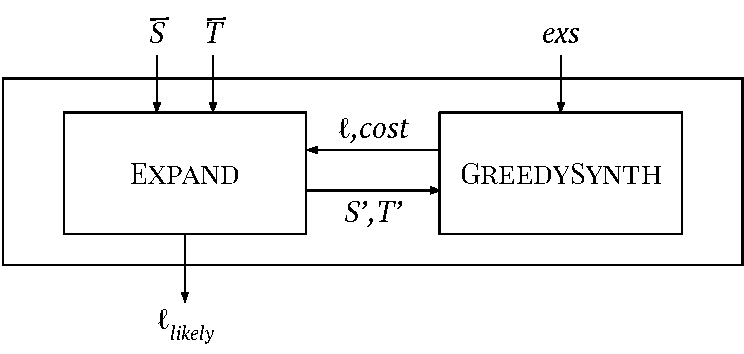
\includegraphics[width=.5\textwidth]{high-level-algorithm.pdf}
  \caption{Schematic diagram for our symmetric lens synthesis algorithm. Regular
    expressions \Regex and \RegexAlt, and a set of examples \Examples, are
    provided as input. \Expand searches through stochastic regular expression
    pairs, equivalent to the originals, and proposes them to \GreedySynth.
    \GreedySynth finds a lens, typed between the generated equivalent pairs.
    When the algorithm determines it has an optimal lens, it returns
  that lens. \ksf{Figure needs to be changed to call first search
  Expand; Are the S and T regular expressions (which should have bars)
  or stochastic regular expressions (which should be called such)?}}
  \label{fig:high-level-algorithm}
\end{figure}

With simple symmetric lenses and SREs in hand, we develop a new algorithm for
synthesizing likely lenses, based on the previous algorithm for synthesizing
bijective lenses. This algorithm is constructed from \Expand and \GreedySynth,
a pair of collaborating search procedures, shown in
Figure~\ref{fig:high-level-algorithm}. Given source and target SREs $S$ and $T$,
the \Expand searches for two \emph{related} SREs $S'$ and $T'$ that are
\emph{compatible} (a heuristic that estimates the likelihood our second
algorithm will succeed). $S'$ and $T'$ are related in the sense that they define
the same regular sets as $S$ and $T$ (respectively) and the distribution of
strings is identical. Indeed, we guarantee these two properties by implementing
a search procedure that obeys the star semi-ring axioms of regular expression
equivalence, and which we show does not alter the probability distributions of
the languages.

Given the two compatible SREs, \GreedySynth uses a greedy, type-directed
algorithm find a likely lens between them. If algorithm estimates that the lens
it has discovered is more likely than any future lens it can possibly find, the
search terminates. Otherwise, this lens is stored away (if it is the best found
so far) and the search continues with \Expand again.

We implemented the \GreedySynth and \Expand algorithms and evaluated their
effectiveness of synthesizing synchronization functions on a range of
benchmarks, including data cleaning tasks taken from Flash Fill, information
extraction tasks taken from Augeas, and ad-hoc format synchronization tasks
taken from a variety of locations\footnote{The majority of these format
  synchronization tasks were found from the following index:
  \url{http://fileformats.archiveteam.org/wiki/Electronic_File_Formats}}.

In summary, our main contributions are:
\begin{itemize}
\item We define the space of simple symmetric lenses, which lies between
  asymmetric lenses and full symmetric lenses and has the useful property that
  its members don't have any internal state (\S\ref{sec:overview}). We describe
  a language for simple symmetric string lenses and the cost metric for that
  language (\S\ref{sec:ssl}).
\item We show how to synthesize simple symmetric lenses (including all
  asymmetric lenses as a special case), using a novel application of stochastic
  regular expressions to guide the search process (\S\ref{sec:synthesis}). In
  particular, we show that the RE star semi-ring equivalences remain valid when
  their semantics are enriched by distributions (\S\ref{sec:sre}).
\item We extend the Boomerang implementation with simple symmetric lenses,
  showing that they can easily be combined with a rich variety of other lens
  extensions including quotients and matching lenses. We evaluate our
  implementation over a set of benchmarks drawn from data cleaning, information
  extraction, and file synchronization tasks and demonstrate that we can
  synthesize all of them in under half a minute (\S\ref{sec:evaluation}).
%
  We also analyze the gap between simple and full symmetric lenses
  empirically and argue that simple ones suffice for many applications.
\item We show that the class of simple lenses can be characterized semantically
  as the subset of full symmetric lenses for which a simple ``forgetfulness''
  property holds (\S\ref{sec:relationship}).
\end{itemize}
We finish the paper with a discussion of related work (\S\ref{sec:related}) and
our final thoughts (\S\ref{sec:conc}).

%Such synthesis efforts
%make it easier to use lenses as programmers do not need to be familiar with the syntax
%of a new language, and even advanced users can benefit from the productivity boost.

\noindent

% state of the world
% end introduction

% begin overview
\section{Overview}
\label{sec:overview}

\begin{figure}
  % https://tex.stackexchange.com/questions/168741/showing-two-listings-in-a-table-side-by-side
  \setbox0=\hbox{%
    \begin{minipage}{3.5in}
\begin{lstlisting}[
stringstyle=\upshape\sffamily
]
Jane Doe: 38000
John Public: 37500
\end{lstlisting}
    \end{minipage}
  }
  \savestack{\listingA}{\box0}

  \setbox0=\hbox{%
    \begin{minipage}{3.5in}
\begin{lstlisting}[
stringstyle=\upshape\sffamily
]
Name,Company
Jane Doe,Healthcare Inc.
John Public,Insurance Co.
\end{lstlisting}
    \end{minipage}
  }
  \savestack{\listingB}{\box0}

  \setbox0=\hbox{%
    \begin{minipage}{3.5in}
\begin{lstlisting}
let salary = number | "unk"
let emp_salary = name . " " . name . ": " salary
let emp_salaries = "" | emp_salary . ("\n" emp_salary)*
\end{lstlisting}
    \end{minipage}
  }
  \savestack{\listingC}{\box0}

  \setbox0=\hbox{%
    \begin{minipage}{3.5in}
\begin{lstlisting}
let company = (name . ("Co." | "Inc." | "Ltd.")) | "UNK" in
let emp_ins = name . " " . name "," company in
let header = "Name,Company" in
let emp_insurance = header . ("\n" . emp_ins)*
\end{lstlisting}
    \end{minipage}
  }
  \savestack{\listingD}{\box0}
  
  \centering
  \resizebox{\columnwidth}{!}{%
    \begin{tabular}{|>{\columncolor{vlightyellow}}c|>{\columncolor{vlightgreen}}c|}
      \hline
      \texttt{company.mgmt} data file & \texttt{company.hr} data file \\
      \hline
      \listingA & \listingB \\
      \hline
      \cellcolor{lightyellow}\texttt{company.mgmt} regular expression & 
      \cellcolor{lightgreen}\texttt{company.hr}  regular expression\\
      \hline
      \cellcolor{lightyellow}\listingC & \cellcolor{lightgreen}\listingD \\
      \hline
    \end{tabular}
  }
  \caption{Hypothetical example data files and corresponding regular expressions
  used by management and HR at a US company to represent employee salaries and health
  insurance providers, respectively. }  
  \label{fig:minimized-representations}
\end{figure}

In this section, we give an overview of simple symmetric lenses and our
synthesis algorithm for them, using a simplified example drawn from a hypothetical
U.S. company. In this company, management and human resources (HR) store
information about employees in separate text files: management records the
names of 
employees and their salaries while HR stores the names of employees and their
health insurance providers. Figure~\ref{fig:minimized-representations} gives
examples of the two file formats and regular expressions describing them. 

The company uses a simple symmetric lens to keep these files
synchronized. If management adds a new employee, ``Chris Roe: 32500'', a lens
adds the corresponding entry ``Chris Roe, UNK'' to HR's file. The sentinel value
``UNK'' represents the fact that the employee's insurance company is currently
unknown. A similar update happens if HR adds a new employee before management,
in which case the sentinel value ``unk'' reflects the unknown salary information
Furthermore, if HR corrects an error in an employee's name, say changing ``John
Public'' to ``Jon Public'', the lens mirrors that name change in management's
file. Not all the data is mirrored, however. The management file is not updated
in response to insurance changes, and the HR file is oblivious to salary
changes. Simple symmetric lenses are appropriate for keeping these two files
synchronized because the files have a mix of shared and unshared information.

%Consider the previously
%described goal of keeping Linux cron jobs (crontab) and Windows Scheduled Tasks
%(scheduled.job) synchronized. These are each formats specifying when to run
%recurring tasks. For the sake of exposition, we use simplified versions crontab
%and scheduled.job formats, with examples and corresponding regular expressions
%shown in Figure~\ref{fig:minimized-representations}. Each file contains a list
%of tasks set to run at specific times every hour. In both formats, users
%can either provide specific minutes at which they want the program to run, or they
%can specify that the program should run at every minute.
%
%We wish for the jobs to be synchronized across our Windows and Linux devices.
%However, the commands that need to be run are typically different for each
%device. Paths are different in Windows and Linux, and, while there is typically a
%Windows equvialent for a Linux command, that equivalent command is not always
%named the same thing. So, while we want to be able to have the same number of
%commands, with the commands running at the same times, we don't want to
%align the actual commands that are run.

\subsection{Simple Symmetric Lenses}
A simple symmetric lens between formats described by types $X$ and $Y$ is
defined by four functions.\bcp{I think a picture would be helpful. I can
  probably make one pretty easily by tweaking the one from the original
  symmetric paper.} \afm{That would be awesome.}

%\begin{enumerate}
%\item $\CreateR \OfType \Regex \rightarrow \RegexAlt$
%\item $\CreateL \OfType \RegexAlt \rightarrow \Regex$
%\item $\PutR \OfType \Regex \rightarrow \RegexAlt \rightarrow \RegexAlt$
%\item $\PutL \OfType \RegexAlt \rightarrow \Regex \rightarrow \Regex$
%\end{enumerate}

\begin{gather}
 \tag{1}
 \mbox{$\CreateR \OfType X \rightarrow Y$}\\
 \tag{2}
 \mbox{$\CreateL \OfType Y \rightarrow X$}\\
 \tag{3}
 \mbox{$\PutR \OfType X \rightarrow Y \rightarrow Y$}\\
 \tag{4}
 \mbox{$\PutL \OfType Y \rightarrow X \rightarrow X$}
\end{gather}

\noindent
that collectively satisfy four ``round-tripping'' laws: 
\begin{gather}
  \tag{\CreatePutRL}
  \PutLOf{(\CreateROf{x})}{x} = x\\
  \tag{\CreatePutLR}
  \PutROf{(\CreateLOf{y})}{y} = y\\
  \tag{\PutRL}
  \PutLOf{(\PutROf{x}{y})}{x} = x\\
  \tag{\PutLR}
  \PutROf{(\PutLOf{y}{x})}{y} = y
\end{gather}
\noindent
The two {\sc Create} functions propagate shared information and fill in default
values when introducing new data. (\EG, the ``unk'' salary entry is added
alongside the name to the management file when HR inserts a new employee). The
two {\sc Put} functions propagate edits from one format to the other by
combining the change from one file with the previous value from the other file.
The roundtripping laws guarantee that if two formats are already synchronized,
{\sc Put}s merely return the second argument, unchanged.

This definition differs from previous formulations of simple symmetric lenses,
as previous formulations required a \emph{complement}. Instead of comprising
four functions, existing formulations merely comprised two functions, which
combined complements with edited formats to create updated complements and
synchronized data. We provide a detailed comparison to classic symmetric lenses
in \S\ref{sec:relationship}.

%%For synchronization, when the original company.hr or company.mgmt
%%file is created, a synchronized file of the other form is created
%%from it with $\CreateR$ or $\CreateL$ (depending on which file was
%%initially created). On future edits, changes are made with the puts,
%%a \PutR would propagate the shared information from the company.hr
%%file, and knit it together with the information specific to the company.mgmt file.


\subsection{Simple Symmetric Lens Combinators}




Generally, we do not expect programmers to define simple symmetric lenses by
writing the four functions by hand and showing they satisfy the roundtripping
laws. Instead, we provide simple symmetric lens combinators to build up the
requisite lenses from simpler ones, and focus our combinators on providing
lenses between string data formats.

We use regular expressions to denote the types of data formats, and we impose a
typing discipline on our lenses. Specifically, if $\BRegex$ and $\BRegexAlt$ are
regular expressions\footnote{We use \BRegex and \BRegexAlt to denote regular
  expressions. We later use the plain nonterminals \Regex and \RegexAlt for
  stochastic regular expressions.}, then the notation
\lstinline{$\Lens$ : $\BRegex \Leftrightarrow \BRegexAlt$} indicates that $\Lens$ is a simple symmetric lens between $\LanguageOf{\BRegex}$ and $\LanguageOf{\BRegexAlt}$. When clear from context, we use the term \textit{lens} to denote a simple symmetric lens.

We briefly explain a selection of these
combinators by using them to define a lens between the two employee data formats
in Figure~\ref{fig:minimized-representations}. The finished lens, which appears
in Figure~\ref{fig:example_lens}, has the type
\lstinline{emp_salaries} $\Leftrightarrow$
\lstinline{emp_insurance}, where
\lstinline{emp_salaries} and
\lstinline{emp_insurance} are regular expressions defined in Figure~\ref{fig:minimized-representations}.


The simplest combinator is the identity lens \IdentityLens, which takes as an
argument a regular expression $\BRegex$ and performs an identity mapping on data
matching $\BRegex$. The identity lens fully connects the
corresponding data in the two formats: when one format is
updated, the other format gets the exact same value. In our example,
when a \lstinline{name} is updated in one file, the identity lens ensures it is
also updated in the other file. In this manner, both the \CreateR and \CreateL
functions are the identity function ($\CreateR \App s = s$), and the put
functions merely return the first argument ($\PutROf{s_1}{s_2} = s_2$).

%
\begin{lstlisting}
id(name) : name $\Leftrightarrow$ name
\end{lstlisting}
%

In contrast to the identity lens, the \Disconnect lens does not propagate edits
from one format to the other. The disconnect lens takes four arguments: two
regular expressions and two strings. The regular expressions specify the formats
of the corresponding data on the two sides while the strings provide default
values. On creates, the input values are thrown away, and default values are
returned ($\CreateROf{\String} =
\lstinline{"unk"}$), and on puts, the second argument is used, and the first is
thrown away ($\PutROf{\String}{\StringAlt} = \StringAlt$). In our extended
example, the \lstinline{salary} field is only present in management files,
so we use the disconnect lens to ensure salary edits do not cause updates to the
HR file.
The defaults are strings that indicate the information is missing.
%
\begin{lstlisting}
disconnect(salary, "", "unk", "") : salary $\Leftrightarrow$ company
\end{lstlisting}
%
The insert \lstinline{ins} and delete \lstinline{del} lenses are
syntactic sugar for uses of the disconnect lens in which a string
constant is omitted entirely from the source and target formats,
respectively.
\begin{lstlisting}
 ins($t$) = disconnect("", $t$, "", $t$)
 del($s$) = disconnect($s$, "", $s$, "")
\end{lstlisting}

Finally, there are a number of standard lenses that compositionally construct
more complex lenses from simpler ones. These combinators include concatenation
($\ConcatLensOf{\Lens_1}{\Lens_2}$ or $\Lens_1 . \Lens_2$), variation
($\OrLensOf{\Lens_1}{\Lens_2}$), and iteration ($\IterateLensOf{\Lens}$).  For example;
%
\begin{lstlisting}
id(name) . ins(",") . id(name) . del(": ") . ins(",")
\end{lstlisting}
% concat(ins(header),employees_lens) : emp_salaries $\Leftrightarrow$ emp_insurance
%
appears in the definition of the \lstinline{name_lens} in our running example.
%\ksf{I don't think this example is necessary.}
%Data can also appear in multiple forms. For example,
%a list of employees with insurance information can either be empty or
%be a sequence of employee/insurance records: \ksf{This example is
%vacuous as you could eliminate the or in favor of the *.  Do somethign
%else to introduce or?}
%
%\begin{lstlisting}
%or(id(""),employees_lens) : emp_salaries $\Leftrightarrow$ "" | ("\n" emp_ins) . ("\n" emp_ins)*
%\end{lstlisting}
The \IterateLens lens also appears in our running example, where it
synchronizes data for a list of employees when given a
lens \lstinline{employee_lens} that synchronizes  data for a single employee:
%
\begin{lstlisting}
iterate(id("\n") . employee_lens) : ("\n" . emp_salary)$^*$ $\Leftrightarrow$ ("\n" . emp_ins)$^*$
\end{lstlisting}
%

\begin{figure}
\begin{lstlisting}
let name_lens = id(name) . ins(",") . id(name) . del(": ") . ins(",") in
let employee_lens = name_lens . disconnect(salary,"","unk","") 
                                                    . disconnect("",company,"","UNK") in
let employees_lens = ins("\n") . employee_lens . iterate(id("\n") . employee_lens) in
ins(header) . employees_lens : emp_salaries $\Leftrightarrow$ emp_insurance
\end{lstlisting}
%\ksf{I don't think this is necesssary.}
%let emp_lens = or(id(""),employees_lens) in
  \caption{A lens, written in our language for building simple symmetric lenses
    on string data, that synchronizes management and HR employee files.
    Note that we can annotate our lenses with types, to confirm the lens
    operates on the languages of the regular expressions. In this work, we
    synthesize the lens itself from such regular expressions.}
  \label{fig:example_lens}
\end{figure}

% Using these combinators, we can build up a lens that synchronizes
% management and HR employee files. 


We provide typing rules for each of the simple symmetric combinators, most of
which are syntax directed. However, regular expressions have a number of
equivalences on them, and sometimes we must convert one regular expression type
to another, equivalent, regular expression type. Our typing rules include type
equivalence, so if a lens has type $\BRegex \Leftrightarrow \BRegexAlt$, then it
is also has type $\BRegex' \Leftrightarrow \BRegexAlt'$, where $\BRegex$ is
equivalent to $\BRegex'$, and $\BRegexAlt$ is equivalent to $\BRegexAlt'$. The
flexibility this type equivalence rule provides is useful when a different
representation of a regular expression would facilitate synthesis.

%%\ksf{Do we need to use
%%type equivalence to type the employee example?  If so, perhaps we
%%should explain her}
%%
%%This lens uses one typing rule not previously
%%mentioned: type equivalence. While \lstinline{scheduled_job} is a equivalent to
%%a regular expression with an outermost disjunction, it is not syntactically
%%equivalent to one. Without type equivalence, the provided lens wouldn't actually
%%be well-typed, but type equivalence states that if a lens is typed between a
%%pair of regular expressions, it is also typed between an equivalent pair.


\subsection{Synthesizing Symmetric Lenses}

While our example is relatively simple for demonstration, writing such lenses
for real-world formats is quite difficult, as these formats can be large and
represent data in complex and unintuitive ways. To alleviate the difficulty of
manually writing simple symmetric lenses, we wish to synthesize them instead.
Given a pair of regular expressions and a set of input-output examples, we want
to find a simple symmetric lens that is typed by the regular expression pair and
satisfies the input/output examples. We call such a lens a \emph{satisfying
  lens}. In our running example, we wish to synthesize a lens between
\lstinline{emp_salaries} and \lstinline{emp_insurance}, using as an input-output
example the data in Figure~\ref{fig:minimized-representations}. The algorithm
uses such examples to find suitable defaults for \Disconnect lenses and to
figure out how to match data that could be synchronised in multiple ways.

A challenge is that the simple symmetric lens combinators permit many
well-typed lenses
between a given pair of regular expressions. For example, 
Figure~\ref{fig:example_lens} gives one possible lens between regular
expressions  \lstinline{emp_salaries} and \lstinline{emp_insurance},
but 
%
\begin{lstlisting}
disconnect(emp_salaries,emp_insurance,rep(emp_salaries),rep(emp_insurance))
\end{lstlisting}
%
is another valid lens (where \lstinline{rep($\BRegex$)} denotes some string in the
language of $\BRegex$). Furthermore, adding the input-output example in
Figure~\ref{fig:minimized-representations} 
helps, but only a little: it may, in general, require {\em many} examples to rule
out all possible occurrences of nested \Disconnect lenses,
particularly in complex formats. 
%\ksf{I don't understand the following.  We shouldn't explain the issue in
%terms of \PutR and \PutL as we are focused on the combinators rather
%than the raw functions.}
%The default strings given to \Disconnect merely need to be the strings
%in the input-output examples, and the lens will still satisfy the
%specification.  While the disconnect lens is prohibited by two
%examples, or by a carefully chosen input-output example on \PutR
%or \PutL, this problem continues presenting itself for the sublenses,
%and is highlighted even more on larger formats.
While we could ask programmers to provide detailed and precise specifications
for their synthesis tasks, we would prefer an algorithm that can intelligently
choose a lens despite the underspecification. Instead of merely finding
\emph{any} satisfying lens, we wish to synthesize a satisfying lens that is
likely to please the user.

But what is a ``likely'' satisfying lens? We propose the following
heuristic: a satisfying
lens is more likely if it connects more data between the two
formats, \EG, by using an identity rather than a disconnect lens.  The
likeliest satisfying lenses would connect as much data as
possible. More formally, we define the likelihood of a
satisfying lens as the expected number of bits required to recover
data in one format from synchronized data in the other.  Higher
likelihoods correspond to lower numbers of bits. In more
detail, we say that two strings $s$ and $t$ are \emph{synchronized
according to lens $l$} if $l.\PutR\ s\ t = t$ and $l.\PutL\ t\ s = s$.\footnote{
The notation $l.\PutR$ extracts the \PutR function from simple
symmetric lens $l$; similarly for \PutL.}  We say that we
can \emph{recover} $s$ from $t$ using bits $b$ and lens $l$ if we can
reconstruct $s$ from $t$, $b$, and $l$.  For example, given
the \IdentityLens{} lens, we can recover $s$ from $t$ using no bits
because, in this case, $s$ is just $t$.  In contrast, given
the \Disconnect{} lens, we need enough bits to fully encode $s$ in
order to recover it from $t$ because $t$ contains no useful
information.  This calculation shows that if both \IdentityLens{}
and \Disconnect{} are satisfying lenses, then \IdentityLens{} is more
likely.

The expected number of bits required to recover data is a well-known concept in
information theory: it is the \emph{entropy} of the data. \saz{Cite Shannon?} Calculating the
entropy of data requires a probability distribution over the space of possible
values for the data. Specifically, given a set $S$ and a probability
distribution over that set $P \OfType S \rightarrow \Reals$, the entropy of $S$
with probability distribution $P$ is $-\Sigma_{s\in S}P(s)\Log_2P(s)$.

In our setting, we already have a way of expressing sets of data:
regular expressions.  What we need is a way to express probability
distributions over that data.
To that end, we adopt \emph{stochastic regular expressions}~\cite{?} (SREs), 
which are regular expressions where each operator is annotated with a
probability.  A stochastic regular expression
specifies both a set of strings and a probability
distribution over it.  From this information, we can calculate the
entropy of the SRE. 

This infrastructure gives us what we need to find likely satisfying lenses from
a collection of satisfying lenses. All such lenses must synchronize data between
the same two SREs $\Regex$ and $\RegexAlt$. For any such lens $\Lens$, we can
calculate the expected number of bits required to recover a string $t$ in
$\LanguageOf{\RegexAlt}$ from a synchronized string $s$ in
$\LanguageOf{\Regex}$. This expectation is the \emph{conditional entropy of
  $\Regex$ given $\RegexAlt$ and $\Lens$}, formally $\sum_{s \in
  \Regex}\ProbabilityOf{\Regex}{s}*\EntropyOf{\SetOf{t \SuchThat
    \Lens.\PutROf{s}{t} = t}}$. The likelihood we assign to $\Lens$ is the sum
of the conditional entropy of $\Regex$ given $\RegexAlt$ and $\Lens$ and the
conditional entropy of $\RegexAlt$ given $\Regex$ and $\Lens$. This metric
assigns higher cost to lenses where knowing the string present in \Regex
provides little information about what string is present in \RegexAlt. With this
metric, bijections have zero cost---given a string $s \in \Regex$, we know
exactly what string is present in $\RegexAlt$, as exactly one string is
synchronized to it.

To obtain SREs from the plain regular expressions that we expect users to
supply, we use a heurstic that attempts to assign probability annotations that
give each string in the language equal probablity. Our algorithm could also take
as input a stochastic regular expression rather than a plain one, which allows
the user to specify a data-specific probability distribution, either manually
written or inferred from a large dataset. We found our heuristically chosen
distribution works well in practice.

Now that we have a way to calculate likelihood, we need a way to search for
likely lenses. Previous work on synthesis~\cite{augustsson-2004,osera+:pldi15,feser-pldi-2015,frankle+:popl16} has shown that we can use
types to dramatically restrict the search space and improve the effectiveness of
synthesis. In our setting, types are pairs of stochastic regular expressions,
which come with a rich algebraic structure that makes each regular expression
semantically equal to infinitely many others. To tame that search space and
leverage the benefits of type-directed synthesis, we split our algorithm into
two communicating synthesizers following earlier
work~\cite{maina+:quotient-synthesis}. The first synthesizer, \Expand, navigates
the space of semantically equivalent regular expressions by applying rewrite
rules that preserve both the semantics and the probability distributions of
those stochastic regular expressions. Our algorithm ranks pairs of stochastic
regular expressions by the number of rewrite rule applications required to
obtain the pair from the stochastic regular expressions given as input. It
passes the pairs off to the second synthesizer, \GreedySynth, in rank order with
the smallest first.

At a high level, \GreedySynth looks for lenses between a given pair of
stochastic regular expressions $\Regex$ and $\RegexAlt$ that have the highest
likelihood by performing a type-directed search. In more detail, \GreedySynth
first normalizes the stochastic regular expressions provided by \Expand into
\emph{stochastic DNF regular expressions}. These stochastic DNF regular
expressions are, intuitively, stochastic regular expressions with disjunctions
distributed over concatenations, where associativity information has been
removed. Then, \GreedySynth uses the syntax of these n-ary DNF regular
expressions to find highly normalized lenses, in a form we call \emph{simple
  symmetric n-ary DNF lenses}. These lenses include neither a composition
operator nor a type equivalence rule. These restrictions mean that each simple
symmetric n-ary DNF lens is typed by a single pair of stochastic n-ary DNF
regular expressions and \GreedySynth's search space for a given pair of regular
expressions is finite. The variations that \GreedySynth considers include
choosing between \IdentityLens{} and \Disconnect lenses and deciding how to
match multiple occurrences of the same kind of data, \EG, the two occurrences of
\lstinline{name} in the management and HR data formats (we want to map first
names to first names and last names to last names). Finally, \GreedySynth
converts this lens back into a simple symmetric lens by converting the n-ary
forms into the binary forms provided in the surface language.

As an example of the partnership between \Expand and \GreedySynth,
consider the lens shown in Figure~\ref{fig:example_lens}. 
Inferring this lens requires \Expand to use a star semiring axiom to
rewrite the regular expression \lstinline{("\n" . emp_salary)$^*$} within
\lstinline{emp_salaries} into 
\lstinline{"" | (("\n" . emp_salary). ("\n" . emp_salary)$^*$)} 
so that \GreedySynth can find the appropriate lens.  

Our strategy of communicating synthesizers gives us a way to
enumerate pairs of stochastic regular expressions of increasing
rank and to efficiently search through them, but it poses a
problem: when do we stop? We may have found a promising lens
between a pair of stochastic regular expressions, but a different 
pair we haven't yet discovered may give rise to an even better lens. 
Or, we may have found a promising lens between a given pair of
stochastic regular expressions, but the discovered lens is not 
acceptable to the users. 

Our algorithm must resolve a three-way tension between the quality of
the inferred lens, the number of examples the user must provide to
eliminate unwanted lenses, and the amount of time it takes to return a
result.  For example, if the algorithm has already found the lens in
Figure~\ref{fig:example_lens}, we don't want to spend a lot of time
searching for an even better lens.

To resolve this tension, our algorithm uses heuristics to judge whether to
return the current best satisfying lens to the user or to pass the
next set of unrollings to \GreedySynth.
The heuristics favor stopping if the current best satisfying
lens has relatively high likelihood, indicating the lens is very promising.
The heuristics also favor stopping if \Expand
has delievered to \GreedySynth all pairs of stochastic regular
expressions at a given rank and there is a large number of pairs at the next
rank because searching through all such pairs will take a long time.
With this approach, the algorithm can quickly respond with a satisfying
lens with relatively high likelihood.  If users are unhappy with the result, they can refine the
search by supplying additional examples, which serve both to rule out
the previously proposed lens(es) and to reduce the size of the search
space by cutting down on the number of satisfying lenses.


%Consider the trivial lens
%\lstinline{disc(emp_salary,emp_row,rep(emp_salary),rep(emp_row))}. As this is
%the disconnect lens, the cost of each side is the entropy of the data format, so
%the total cost is $\EntropyOf{\lstinline{emp_salary}} +
%\EntropyOf{\lstinline{emp_row}}}$. \lstinline{emp_salary} contains strictly more
%imformation than \EntropyOf{\lstinline{": " . salary}}, and \lstinline{emp_row}
%contains strictly more information than \EntropyOf{\lstinline{": " . salary}},
%so by our metric \lstinline{single_emp_map} is preferable to the disconnect
%lens.

%Not sure we need this level of detail after all.
%\afm{calculations for cost of various lenses between \lstinline{emp_salary} and
%  \lstinline{emp_row}} Consider the lens \lstinline{single_emp_map} between
%\lstinline{emp_salary} and \lstinline{emp_row}. Given this lens, the expected
%entropy of recovering the left format from the right
%($\EntropyOf{\lstinline{emp_salary} \Given \lstinline{emp_row},
%  \lstinline{single_emp_map} }$) is the sum of the expected entropy of
%recovering each of its subcomponents, $\EntropyOf{\lstinline{emp_salary} \Given
%  \lstinline{emp_row}, \lstinline{single_emp_map} } = \EntropyOf{\lstinline{name
%    . " " . name} \Given \lstinline{name . "," . name}, \lstinline{name_map}
%}$\\ + $\EntropyOf{\lstinline{": " . salary} \Given
%  \lstinline{"," . company}, \lstinline{disc(salary,company,"UNSET","UNSET")}
%}$.
%
%The entropy of the identity lens is zero. As the two formats are in bijective
%correspondence, we know exactly which string is present in the left-hand format.
%The entropy of the disconnect lens is just the entropy of
%\lstinline{": " . salary}.  Knowing which string is present in the right-hand
%format tells us nothing about what string is present in the left-hand format. So
%$\EntropyOf{\lstinline{emp_salary} \Given \lstinline{emp_row},
%  \lstinline{single_emp_map} } = \EntropyOf{\lstinline{": " . salary} }$
%
%Analogously, $\EntropyOf{\lstinline{emp_row} \Given \lstinline{emp_salary},
%  \lstinline{single_emp_map} }$ is just $\EntropyOf{\lstinline{"," . company}
%}$, so the total cost of the lens is $\EntropyOf{\lstinline{": " . salary}} +
%\EntropyOf{\lstinline{"," . company}}$

%Consider the trivial lens
%\lstinline{disc(emp_salary,emp_row,rep(emp_salary),rep(emp_row))}. As this is
%the disconnect lens, the cost of each side is the entropy of the data format, so
%the total cost is $\EntropyOf{\lstinline{emp_salary}} +
%\EntropyOf{\lstinline{emp_row}}$. \lstinline{emp_salary} contains strictly more
%imformation than \EntropyOf{\lstinline{": " . salary}}, and \lstinline{emp_row}
%contains strictly more information than \EntropyOf{\lstinline{": " . salary}},
%so by our metric \lstinline{single_emp_map} is preferable to the disconnect
%lens.
Consider the trivial lens
\lstinline{disc(emp_salary,emp_row,rep(emp_salary),rep(emp_row))}. As this is
the disconnect lens, the cost of each side is the entropy of the data format, so
the total cost is $\EntropyOf{\lstinline{emp_salary} } +
\EntropyOf{\lstinline{emp_row}}$. \lstinline{emp_salary} contains strictly more
information than $\EntropyOf{\lstinline{": " . salary}}$, and
\lstinline{emp_row} contains strictly more information than
\EntropyOf{\lstinline{": " . salary}}, so by our metric
\lstinline{single_emp_map} is preferable to the disconnect lens.
% end overview

% begin stoch-rx
% end stoch-rx

\section{Stochastic Regular Expressions}
\label{sec:sre}
To characterize the likely lenses, we must compute the expected number of bits
needed to recover a string in one data source from a synchronized string in the
other data source. To do this, we must first develop a probabilistic language
model for our language. We do this with \emph{stochastic regular expressions},
regular expressions annotated with probability information. With this, we can
jointly express a language and a probability distribution over that language. In
the following grammar, $\String$ ranges over strings, and $\Probability$ ranges
over real numbers between 0 and 1, exclusive.

$$\Regex{},\RegexAlt{} \GEq{}  \String  \; | \; \emptyset \; | \; \PRegexStar{\Regex}{p} \; | \; \RegexConcat{\Regex_1}{\Regex_2} \; | \; \PRegexOr{\Regex_1}{\Regex_2}{p}$$

In the stochastic regular expression
$\PRegexOr{\Regex_1}{\Regex_2}{\Probability}$, the annotation $\Probability$
represents the likelihood the string is in $\Regex_1$. In the stochastic regular
expression $\PRegexStar{\Regex}{\Probability}$, the annotation \Probability how
much more likely having a string involving more than $n$ iterations is than
having a string involving exactly $n$ iterations. The semantics of SREs is
defined by the function $P$ below.

\begin{center}
  \begin{tabular}{rcl}
    $\ProbabilityOf{\String}{\String''}$
    & =
    & $\begin{cases*}1 & if $\String = \String''$\\ 0 & otherwise\end{cases*}$ \\
     
    $\ProbabilityOf{\emptyset}{\String}$
    & =
    & $0$ \\
    
    $\ProbabilityOf{\RegexConcat{\Regex_1}{\Regex_2}}{s}$

    & =
    & $\Sigma_{\String = \String_1\String_2}\ProbabilityOf{\Regex_1}{\String_1}*\ProbabilityOf{\Regex_2}{\String_2}$ \\
    
    $\ProbabilityOf{\PRegexOr{\Regex_1}{\Regex_2}{\Probability}}{\String}$
    & =
    & $\Probability * \ProbabilityOf{\Regex_1}{\String} +
      (1-\Probability) * \ProbabilityOf{\Regex_2}{\String}$\\
    
    $\ProbabilityOf{\PRegexStar{\Regex}{\Probability}}{\String}$
    & =
    & $\Sigma_n \Sigma_{\String = \String_1 \ldots \String_n}\Probability^n*(1-\Probability)*\Pi_{i=1}^n\ProbabilityOf{\Regex}{\String_i}$\\
  \end{tabular}
\end{center}

\subsection{Stochastic Regular Expression Equivalences}
$\Expand$ needs to be able to find equivalent stochastic regular expressions.
However, existing work does not provide a means to reason about stochastic
regular expression equivalence. We extend the \emph{star-semiring}~\cite{?}
equivalences to stochastic regular expressions.

\begin{center}
  \begin{tabular}{@{}r@{\hspace{1em}}c@{\hspace{1em}}l@{}r@{}}
    \PRegexOr{\Regex}{\emptyset}{1} & $\SSREquiv$ & \Regex{} & \OrIdentityRule{} \\
    $\RegexConcat{\Regex}{\emptyset}$ & $\SSREquiv$ & $\emptyset$ & \EmptyProjectionRightRule{} \\
    $\RegexConcat{\emptyset}{\Regex}$ & $\SSREquiv$ & $\emptyset$ & \EmptyProjectionLeftRule{} \\
    \RegexConcat{(\RegexConcat{\Regex{}}{\Regex'})}{\Regex''} & $\SSREquiv$ & \RegexConcat{\Regex{}}{(\RegexConcat{\Regex'}{\Regex''})} & \ConcatAssocRule{}  \\
    \PRegexOr{(\PRegexOr{\Regex}{\Regex'}{\Probability_1})}{\Regex''}{\Probability_2} & $\SSREquiv$ & \PRegexOr{\Regex}{(\PRegexOr{\Regex'}{\Regex''}{\frac{(1-\Probability_1)*\Probability_2}{1 - \Probability_1 * \Probability_2}})}{\Probability_1*\Probability_2} & \OrAssociativityRule{}  \\
    \PRegexOr{\Regex{}}{\RegexAlt{}}{\Probability} & $\SSREquiv$ & \PRegexOr{\RegexAlt{}}{\Regex{}}{1-\Probability} & \OrCommutativityRule{}\\
    \RegexConcat{\Regex{}}{(\PRegexOr{\Regex{}'}{\Regex{}''}{\Probability})} & $\SSREquiv$ & \PRegexOr{(\RegexConcat{\Regex{}}{\Regex{}'})}{(\RegexConcat{\Regex{}}{\Regex{}''})}{\Probability} & \DistributivityLeftRule{} \\
    \RegexConcat{(\PRegexOr{\Regex{}'}{\Regex{}''}{\Probability})}{\Regex{}} & $\SSREquiv$ & \PRegexOr{(\RegexConcat{\Regex{}'}{\Regex{}})}{(\RegexConcat{\Regex{}''}{\Regex{}})}{\Probability} & \DistributivityRightRule{} \\
    \RegexConcat{\EmptyString{}}{\Regex{}} & $\SSREquiv$ & \Regex{} & \ConcatIdentityLeftRule{} \\
    \RegexConcat{\Regex{}}{\EmptyString{}} & $\SSREquiv$ & \Regex{} & \ConcatIdentityRightRule{} \\
    \PRegexStar{\Regex{}}{\Probability} & $\SSREquiv$ & \PRegexOr{\EmptyString{}}{(\RegexConcat{\Regex{}}{\PRegexStar{\Regex{}}{\Probability}})}{1-\Probability} & \UnrollstarLeftRule{} \\
    \PRegexStar{\Regex{}}{\Probability} & $\SSREquiv$ & \PRegexOr{\EmptyString{}}{(\RegexConcat{\PRegexStar{{\Regex{}}}{\Probability}}{\Regex{}})}{1-\Probability} & \UnrollstarRightRule{} 
  \end{tabular}
\end{center}

\begin{theorem}
  If $\Regex \SSREquiv \RegexAlt$ then $\ProbabilityOf{\Regex}{\String} =
  \ProbabilityOf{\RegexAlt}{\String}$, for all strings $\String \in \LanguageOf{\Regex}$.
\end{theorem}
\begin{proof}
  The proofs of this theorem, and subsequent theorems in this paper, appears in
  the appendix present in the full version of the paper accompanying this
  submission.
\end{proof}

We prove these star-semiring equivalences sound, as those are the equivalences
we either traverse (with \Expand), or normalize across (as part of
\GreedySynth).

\subsection{Stochastic Regular Expression Entropy}
The entropy of a data source $S$ is the expected number of bits required to
describe a random element in $S$ ($-\Sigma_{s\in S}P(s)\Log_2P(s)$). The entropy
of a stochastic regular expression can be computed directly from its syntax,
when the stochastic regular expression is unambiguous and contains no empty
subcomponents.
\begin{center}
  \begin{tabular}{rcl}
    $\EntropyOf{s}$
    & =
    & 1\\
    
    $\EntropyOf{\PRegexStar{\Regex}{\Probability}}$
    & =
    & $\frac{\Probability}{1-\Probability}(\EntropyOf{\Regex} - \Log_2\Probability)
      - \Log_2(1-\Probability)$\\
    
    $\EntropyOf{\PRegexConcat{\Regex}{\RegexAlt}}$
    & =
    & \EntropyOf{\Regex} + \EntropyOf{\RegexAlt}\\
    
    $\EntropyOf{\PRegexOr{\Regex}{\RegexAlt}{\Probability}}$
    & =
    & $\Probability*(\EntropyOf{\Regex} - \Log_2(\Probability)) + (1-\Probability)*(\EntropyOf{\RegexAlt} - \Log_2(1-\Probability))$\\
  \end{tabular}
\end{center}
We have proven that this syntactic computation corresponds to the entropy of the
stochastic regular expression.

\begin{theorem}
  \label{thm:correct_entropy}
  If $\Regex$ is unambiguous and does not contain $\emptyset$ as a subterm,
  $\EntropyOf{\Regex}$ is the entropy of $\Regex$.
\end{theorem}

Without unambiguity constraints it is not easy to calculate the entropy. This
method is certainly incorrect without unambiguity constraints: consider the SRE
$\PRegexOr{\lstinline{"a"}}{\lstinline{"a"}}{.5}$. Using the above computation,s
this SRE has an entropy of $1$, but the entropy should be $0$. These
difficulties become particularlly complex when the languages are ambiguous in
subtle ways, the algorithm must be correct when only some of the two languages
overlap. Similar issues occur when trying to find the entropy when $\emptyset$
is a subterm (what should the entropy of $\PRegexStar{\emptyset}{.5}$ be), so we
do not define the entropy on $\emptyset$.

In our work, these conditions are merely a technicality, we require unambiguous
regular expressions as input to our synthesis procedure, and we can easily
preprocess emptysets out of the stochastic regular expressions that are
themselves nonempty by traversing the correct star-semiring equivalences (\EG,
\PRegexOr{\emptyset}{\lstinline{"s"}}{.5} \SSREquiv \lstinline{"s"}).

% \caption{Regular Expression Equivalences}
% \label{fig:regex-equivalence-rules}

\section{Simple Symmetric String Lenses}
\label{sec:ssl}
\saz{This paragraph used to say that lenses are typed between stochastic REs
  and it also says that lenses are typed between REs.  I think its should just
  be REs? Double check that this is correct} 

We now give a formal description of all the combinators in our symmetric lens
language.  While our algorithms perform synthesis on stochastic regular
expressions, lenses themselves are typed between regular expressions.  We can
recover a regular expression from a stochastic regular expression by deleting
probability annotations.  In a slight abuse of notation\saz{Why is this an
  abuse?}, if $\Regex$ is a stochastic regular expression, $\BRegex$ is the
regular expression obtained by removing probability annotations. The typing
judgment $\Lens \OfType \BRegex \Leftrightarrow \BRegexAlt$ means that $\Lens$
is a well typed lens between $\LanguageOf{\BRegex}$ and
$\LanguageOf{\BRegexAlt}$.

\begin{align*}
\ell ::= &\IdentityLensOf{\BRegex} \; | \; \DisconnectOf{\BRegex}{\BRegexAlt}{\String}{\StringAlt} \; | \; \IterateLensOf{\Lens} \; | \; \ConcatLensOf{\Lens_1}{\Lens_2} \; | \; \SwapLensOf{\Lens_1}{\Lens_2} \; | \; \OrLensOf{\Lens_1}{\Lens_2} \; | \; \ComposeLensOf{\Lens_1}{\Lens_2} \; |\\
&\MergeROf{\Lens_1}{\Lens_2} \; | \; \MergeLOf{\Lens_1}{\Lens_2} \; | \; \InvertOf{\Lens}
\end{align*}

We have already described a number of these lenses in \S\ref{sec:overview}.
The compose lens $\Lens_1 ; \Lens_2$ composes two lenses sequentially, it
transforms from one data format to the other by first transforming to an
intermediate format, shared as the target of $\Lens_1$ and the source of
$\Lens_2$. The \MergeR lens combines two sublenses which share the same target.
Which lens gets used depends on what data is in the left-hand format, if it is
in the domain of $\Lens_1$ then $\Lens_1$ gets used, and similarly for
$\Lens_2$.  The \MergeL lens is symmetric to \MergeR, the two sublenses must
share the same source. Finally, $\InvertOf{\Lens}$ inverts a lens, \CreateR
becomes \CreateL and \PutR becomes \PutL, and vice-versa.

We now provide the typing derivations and semantics for these lenses. For
simplicity of presentation, we define the typing derivations and semantics only
over unambiguous regular expressions, even though some lenses can be defined
over ambiguous regular expressions (for example, the identity lens doesn't need
any ambiguity constraints). We believe relaxing this restriction is
unproblematic.

\begin{centermath}
\begin{array}[b]{l@{\qquad \; \qquad}l}
\begin{array}[b]{c}
\quad\\
  \inferrule*
  {
  }
  {
    \IdentityLensOf{\BRegex} \OfType \BRegex \Leftrightarrow \BRegex
  }
  \\
  \quad
  \end{array}
&
\begin{array}[b]{r@{\ }c@{\ }l}
    \CreateR{} \App s & = & s\\
    \CreateL{} \App s & = & s\\
    \PutR{} \App s_1 \App s_2 & = & s_1\\
    \PutL{} \App s_1 \App s_2 & = & s_1
  \end{array}
\end{array}
\end{centermath}
Note that the identity lens ignores the second argument in the put functions.
Because the two formats are fully synchronized, no knowledge of the prior data
is needed.

\begin{centermath}
\begin{array}[b]{l@{\qquad \; \qquad}l}
  \inferrule*
  {
    \String \in \LanguageOf{\BRegex}\\
    \StringAlt \in \LanguageOf{\BRegexAlt}
  }
  {
    \DisconnectOf{\BRegex}{\BRegexAlt}{\String}{\StringAlt}
    \OfType \BRegex \Leftrightarrow \BRegexAlt
  }
&
  \begin{array}{@{}r@{\ }c@{\ }l@{}}
    $\CreateR{} \App \String'$ & = & $\StringAlt$\\
    $\CreateL{} \App \StringAlt'''''$ & = & $\String$\\
    $\PutR{} \App \String''' \App \StringAlt'$ & = & $\StringAlt'$\\
    $\PutL{} \App \StringAlt' \App \String'$ & = & $\String'$
  \end{array}
\end{array}
\end{centermath}

Just as the identity lens ignores the second argument in puts, disconnect lenses
ignore the first in both puts and creates.  The data is unsynchronized in these
two formats, information from one format doesn't impact the other.

\begin{centermath}
\begin{tabular}[b]{l@{\qquad \; \qquad}l}
$
  \inferrule*
  {
    \Lens_1 \OfType \BRegex_1 \Leftrightarrow \BRegexAlt_1\\
    \Lens_2 \OfType \BRegex_2 \Leftrightarrow \BRegexAlt_2
  }
  {
    \ConcatLensOf{\Lens_1}{\Lens_2} \OfType \BRegex_1 \Concat \BRegex_2
    \Leftrightarrow
    \BRegexAlt_1 \Concat \BRegexAlt_2
  }
$
&
$
  \inferrule*
  {
    \Lens_1 \OfType \BRegex_1 \Leftrightarrow \BRegexAlt_1\\
    \Lens_2 \OfType \BRegex_2 \Leftrightarrow \BRegexAlt_2
  }
  {
    \SwapLensOf{\Lens_1}{\Lens_2} \OfType \BRegex_1 \Concat \BRegex_2
    \Leftrightarrow
    \BRegexAlt_2 \Concat \BRegexAlt_1
  }
$
\end{tabular}
\end{centermath}
%\begin{center}
%  \begin{tabular}{@{}r@{\ }c@{\ }l@{}}
%    $\CreateR{} \App \String_1 \String_2$ & = & $(\Lens_1.\CreateROf{\String_1})(\Lens_2.\CreateROf{\String_2})$\\
%    $\CreateL{} \App \StringAlt_1 \StringAlt_2$ & = & $(\Lens_1.\CreateLOf{\StringAlt_1})(\Lens_2.\CreateLOf{\StringAlt_2})$\\
%    $\PutR{} \App (\String_1\String_2) \App (\StringAlt_1\StringAlt_2)$ & = & $(\Lens_1.\PutROf{\String_1}{\StringAlt_1})(\Lens_2.\PutROf{\String_2}{\StringAlt_2})$\\
%    $\PutL{} \App (\StringAlt_1\StringAlt_2) \App (\String_1\String_2)$ & = & $(\Lens_1.\PutLOf{\StringAlt_1}{\String_1})(\Lens_2.\PutLOf{\StringAlt_2}{\String_2})$\\
%  \end{tabular}
%\end{center}

Concat is similar to concatenation in existing string lens languages like
Boomerang.  For such terms, we do not provide the semantics, and merely refer readers to existing work. The swap combinator is similar to concat, though the second regular expression
is swapped.
%\begin{center}
%  \begin{tabular}{@{}r@{\ }c@{\ }l@{}}
%    $\CreateR{} \App \String_1\String_2$ & = & $(\Lens_2.\CreateROf{\String_2})(\Lens_1.\CreateROf{\String_1})$\\
%    $\CreateL{} \App \StringAlt_2\StringAlt_1$ & = & $(\Lens_1.\CreateLOf{\StringAlt_1})(\Lens_2.\CreateLOf{\StringAlt_2})$\\
%    $\PutR{} \App (\String_1\String_2) \App (\StringAlt_2\StringAlt_1)$ & = & $(\Lens_2.\PutROf{\String_2}{\StringAlt_2})(\Lens_1.\PutROf{\String_1}{\StringAlt_1})$\\
%    $\PutL{} \App (\StringAlt_2\StringAlt_1) \App (\String_1\String_2)$ & = & $(\Lens_1.\PutLOf{\StringAlt_1}{\String_1})(\Lens_2.\PutLOf{\StringAlt_2}{\String_2})$\\
%  \end{tabular}
%\end{center}
\begin{centermath}
\begin{tabular}[b]{l@{\qquad}l}
$
  \inferrule*
  {
    \Lens_1 \OfType \BRegex_1 \Leftrightarrow \BRegexAlt_1\\
    \Lens_2 \OfType \BRegex_2 \Leftrightarrow \BRegexAlt_2
  }
  {
    \OrLensOf{\Lens_1}{\Lens_2} \OfType
    \RegexOr{\BRegex_1}{\BRegex_2}
    \Leftrightarrow
    \RegexOr{\BRegexAlt_1}{\BRegexAlt_2}
  }
  $
&
  \begin{tabular}{@{}r@{\ }c@{\ }l@{}}
    $\CreateR{} \App \String$
    & =
    & $\begin{cases*}
      \Lens_1.\CreateROf{\String} & if $\String\in\LanguageOf{\BRegex_1}$\\
      \Lens_2.\CreateROf{\String} & if $\String\in\LanguageOf{\BRegex_2}$
      \end{cases*}$\\
    
    $\CreateL{} \App \StringAlt$
    & =
    & $\begin{cases*}
      \Lens_1.\CreateLOf{\StringAlt} & if $\StringAlt\in\LanguageOf{\BRegexAlt_1}$\\
      \Lens_2.\CreateLOf{\StringAlt} & if $\StringAlt\in\LanguageOf{\BRegexAlt_2}$
      \end{cases*}$\\
    
    $\PutR{} \App \String \App \StringAlt$
    & =
    & $\begin{cases*}
        \Lens_1.\PutROf{\String}{\StringAlt} & if $\String\in\LanguageOf{\BRegex_1} \BooleanAnd \StringAlt\in\LanguageOf{\BRegexAlt_1}$\\
        \Lens_2.\PutROf{\String}{\StringAlt} & if $\String\in\LanguageOf{\BRegex_2} \BooleanAnd \StringAlt\in\LanguageOf{\BRegexAlt_2}$\\
        \Lens_1.\CreateROf{\String} & if $\String\in\LanguageOf{\BRegex_1} \BooleanAnd \StringAlt\in\LanguageOf{\BRegexAlt_2}$\\
        \Lens_2.\CreateROf{\String} & if $\String\in\LanguageOf{\BRegex_2} \BooleanAnd \StringAlt\in\LanguageOf{\BRegexAlt_1}$
      \end{cases*}$\\
    
    $\PutL{} \App \StringAlt \App \String$
    & =
    & $\begin{cases*}
        \Lens_1.\PutLOf{\StringAlt}{\String} & if $\StringAlt\in\LanguageOf{\BRegexAlt_1} \BooleanAnd \String\in\LanguageOf{\BRegex_1}$\\
        \Lens_2.\PutLOf{\StringAlt}{\String} & if $\StringAlt\in\LanguageOf{\BRegexAlt_2} \BooleanAnd \String\in\LanguageOf{\BRegex_2}$\\
        \Lens_1.\CreateLOf{\StringAlt} & if $\StringAlt\in\LanguageOf{\BRegexAlt_1} \BooleanAnd \String\in\LanguageOf{\BRegex_2}$\\
        \Lens_2.\CreateLOf{\String} & if $\StringAlt\in\LanguageOf{\BRegexAlt_2} \BooleanAnd \String\in\LanguageOf{\BRegex_1}$
      \end{cases*}$\\
  \end{tabular}
\end{tabular}
\end{centermath}
The \OrLens lens deals with data that can come in one form or another. If the
data gets changed from one format to the other, information in the old format is
lost.
%\begin{center}
%  \begin{tabular}{@{}r@{\ }c@{\ }l@{}}
%    $\CreateR{} \App \String_1\ldots\String_n$
%    & =
%    & $(\Lens.\CreateROf{\String_1})\ldots(\Lens.\CreateROf{\String_n})$\\
%    
%    $\CreateL{} \App \StringAlt_1\ldots\StringAlt_n$
%    & =
%    & $(\Lens.\CreateLOf{\StringAlt_1})\ldots(\Lens.\CreateLOf{\StringAlt_n})$\\
%    
%    $\PutR{} \App (\String_1\ldots\String_n) \App (\StringAlt_1\ldots\StringAlt_m)$
%    & =
%    & $\StringAlt_1'\ldots\StringAlt_n'$ where $\StringAlt_i' =
%      \begin{cases*}
%        \Lens.\PutROf{\String_i}{\StringAlt_i} & if $i \leq m$\\
%        \Lens.\CreateROf{\String_i} & otherwise
%      \end{cases*}$\\
%    $\PutL{} \App (\StringAlt_1\ldots\StringAlt_m) \App (\String_1\ldots\String_n)$
%    & =
%    & $\String_1'\ldots\String_n'$ where $\String_i' =
%      \begin{cases*}
%        \Lens.\PutROf{\StringAlt_i}{\String_i} & if $i \leq n$\\
%        \Lens.\CreateROf{\StringAlt_i} & otherwise
%      \end{cases*}$
%  \end{tabular}
%\end{center}
\begin{centermath}
\begin{tabular}[b]{l@{\qquad}l}
$
  \centering
  \inferrule*
  {
    \Lens_1 \OfType \BRegex_1 \Leftrightarrow \BRegexAlt\\
    \Lens_2 \OfType \BRegex_2 \Leftrightarrow \BRegexAlt
  }
  {
    \MergeROf{\Lens_1}{\Lens_2} \OfType
    \RegexOr{\BRegex_1}{\BRegex_2}
    \Leftrightarrow
    \BRegexAlt
  }
$
&
  \begin{tabular}{@{}r@{\ }c@{\ }l@{}}
    $\CreateR{} \App \String$
    & =
    & $\begin{cases*}
      \Lens_1.\CreateROf{\String} & if $\String\in\LanguageOf{\BRegex_1}$\\
      \Lens_2.\CreateROf{\String} & if $\String\in\LanguageOf{\BRegex_2}$
      \end{cases*}$\\
    
    $\CreateL{} \App \StringAlt$
    & =
    & $\Lens_1.\CreateLOf{\StringAlt}$\\
    
    $\PutR{} \App \String \App \StringAlt$
    & =
    & $\begin{cases*}
      \Lens_1.\PutROf{\String}{\StringAlt} & if $\String\in\LanguageOf{\BRegex_1}$\\
      \Lens_2.\PutROf{\String}{\StringAlt} & if $\String\in\LanguageOf{\BRegex_2}$
    \end{cases*}$\\
    
    $\PutL{} \App \StringAlt \App \String$
    & =
    & $\begin{cases*}
        \Lens_1.\PutLOf{\StringAlt}{\String} & if $\String\in\LanguageOf{\BRegex_1}$\\
        \Lens_2.\PutLOf{\StringAlt}{\String} & if $\String\in\LanguageOf{\BRegex_2}$
      \end{cases*}$\\
  \end{tabular}
\end{tabular}
\end{centermath}

The \MergeR lens is interesting because it merges data where one data can be in
two formats, and one data has only one format. In previous work~\cite{?}, this
was combined into \OrLens{}, where \OrLens{} could have ambiguous types, but we
find it more clear to have explicit merge operators: it is easier to see what
lens the synthesis algorithm is creating.

\begin{centermath}
\begin{tabular}[b]{l@{\qquad}l}
$
  \inferrule*
  {
    \Lens_1 \OfType \BRegex \Leftrightarrow \BRegexAlt_1\\
    \Lens_2 \OfType \BRegex \Leftrightarrow \BRegexAlt_2
  }
  {
    \MergeLOf{\Lens_1}{\Lens_2} \OfType
    \BRegex
    \Leftrightarrow
    \RegexOr{\BRegexAlt_1}{\BRegexAlt_2}
  }
$
&
  \begin{tabular}{@{}r@{\ }c@{\ }l@{}}
    $\CreateR{} \App \String$
    & =
    & $\Lens_1.\CreateROf{\String}$\\
    
    $\CreateL{} \App \StringAlt$
    & =
    & $\begin{cases*}
      \Lens_1.\CreateLOf{\StringAlt} & if $\StringAlt\in\LanguageOf{\BRegexAlt_1}$\\
      \Lens_2.\CreateLOf{\StringAlt} & if $\StringAlt\in\LanguageOf{\BRegexAlt_2}$
      \end{cases*}$\\
    
    $\PutR{} \App \String \App \StringAlt$
    & =
    & $\begin{cases*}
      \Lens_1.\PutROf{\String}{\StringAlt} & if $\StringAlt\in\LanguageOf{\BRegexAlt_1}$\\
      \Lens_2.\PutROf{\String}{\StringAlt} & if $\StringAlt\in\LanguageOf{\BRegexAlt_2}$
    \end{cases*}$\\
    
    $\PutL{} \App \StringAlt \App \String$
    & =
    & $\begin{cases*}
        \Lens_1.\PutLOf{\StringAlt}{\String} & if $\StringAlt\in\LanguageOf{\BRegexAlt_1}$\\
        \Lens_2.\PutLOf{\StringAlt}{\String} & if $\StringAlt\in\LanguageOf{\BRegexAlt_2}$
      \end{cases*}$\\
  \end{tabular}
\end{tabular}
\end{centermath}
The \MergeL lens is symmetric to \MergeR.

\begin{centermath}
\begin{tabular}[b]{l@{\qquad}l}
  $
  \inferrule*
  {
    \Lens_1 \OfType \BRegex \Leftrightarrow \BRegexAlt\\
    \Lens_2 \OfType \BRegexAlt \Leftrightarrow \BRegexAltAlt\\
  }
  {
    \ComposeLensOf{\Lens_1}{\Lens_2} \OfType
    \BRegex \Leftrightarrow \BRegexAltAlt
  }
$
&
  \begin{tabular}{@{}r@{\ }c@{\ }l@{}}
    $\CreateR{} \App \String$ & = & $\Lens_2.\CreateROf{(\Lens_1.\CreateROf{\String})}$\\
    $\CreateL{} \App \StringAlt$ & = & $\Lens_1.\CreateLOf{(\Lens_2.\CreateLOf{\StringAlt})}$\\
    $\PutR{} \App \String \App \StringAltAlt$ & = & $\Lens_2.\PutROf{(\Lens_1.\PutROf{\String}{(\Lens_2.\CreateLOf{\StringAltAlt})})}{\StringAltAlt}$\\
    $\PutL{} \App \StringAltAlt \App \String$ & = & $\Lens_1.\PutLOf{(\Lens_2.\PutLOf{\StringAltAlt}{(\Lens_2.\CreateROf{\String})})}{\String}$
  \end{tabular}
\end{tabular}
\end{centermath}
Composing is interesting in the put functions. Because puts require intermediary
data, we recreate that intermediary data with creates.

\begin{centermath}
\begin{tabular}[b]{l@{\qquad}l}
$
\inferrule*
  {
    \Lens \OfType \BRegex \Leftrightarrow \BRegexAlt
  }
  {
    \IterateLensOf{\Lens} \OfType
    \StarOf{\BRegex}
    \Leftrightarrow
    \StarOf{\BRegexAlt}
  }
  $
  &
  $
  \inferrule*
  {
    \Lens \OfType \BRegex \Leftrightarrow \BRegexAlt
  }
  {
    \InvertOf{\Lens} \OfType \BRegexAlt \Leftrightarrow \BRegex
  }
  $
\end{tabular}
\end{centermath}
%\begin{center}
%  \begin{tabular}{@{}r@{\ }c@{\ }l@{}}
%    $\CreateR{} \App \StringAlt$ & = & $\Lens.\CreateLOf{\StringAlt}$\\
%    $\CreateL{} \App \String$ & = & $\Lens.\CreateROf{\String}$\\
%    $\PutR{} \App \StringAlt \App \String$ & = & $\Lens.\PutLOf{\StringAlt}{\String}$\\
%    $\PutL{} \App \String \App \StringAlt$ & = & $\Lens.\PutROf{\String}{\StringAlt}$
%  \end{tabular}
%\end{center}
The \IterateLens lens deals with iterated data, while inverting reverses the direction of a lens: creating on the right becomes creating on the left and vice versa, and putting on the right becomes putting on the left and vice versa. The invert combonator is particularly useful when chaining many compositions together, as it can be used to align the central types.
\[
  \centering
  \inferrule*
  {
    \Lens \OfType \BRegex \Leftrightarrow \BRegexAlt\\
    \BRegex \SSREquiv \BRegex'\\
    \BRegexAlt \SSREquiv \BRegexAlt'
  }
  {
    \Lens \OfType \BRegex' \Leftrightarrow \BRegexAlt'
  }
\]

Type equivalence enables a lens of type $S \Leftrightarrow T$ to be used as a
lens of type $S' \Leftrightarrow T'$ if $S$ equivalent to $S'$ and $T$ is
equivalent to $T'$. Type equivalence is useful both for addressing type
annotations, and for making well-typed compositions.

\subsection{Lens Costs}
Our cost metric is based on the expected amount of information required to
recover a string in one data format from the other. We use the function
$\REntropyOf{\RegexAlt \Given \Lens, \Regex}$ to calculate bounds of the
expected amount of information required to recover a string in $\RegexAlt$ from
a string in $\Regex$, synchronized by $\Lens$. We use the function
$\LEntropyOf{\Regex \Given \Lens, \RegexAlt}$ to calculate bounds of the
expected amount of information required to recover a string in $\Regex$ from a
string in $\RegexAlt$, synchronized by $\Lens$.
\begin{center}
  \begin{tabular}{rcl}
    $\REntropyOf{\RegexAlt \Given \IdentityLensOf{\RegexAlt}, \RegexAlt}$
    & =
    & [0,0]\\
    
    $\REntropyOf{\RegexAlt \Given \DisconnectOf{\Regex}{\RegexAlt}{\String}{\StringAlt}, \Regex}$
    & =
    & [\EntropyOf{\RegexAlt},\EntropyOf{\RegexAlt}]\\

    $\REntropyOf{\PRegexStar{\RegexAlt}{\ProbabilityAlt} \Given \IterateLensOf{\Lens}, \PRegexStar{\Regex}{\Probability}}$
    & =
    & $\frac{\Probability}{1-\Probability}(\REntropyOf{\RegexAlt \Given \Lens, \Regex})$\\
    
    $\REntropyOf{\RegexAlt_1 \Concat \RegexAlt_2 \Given \ConcatLensOf{\Lens_1}{\Lens_2}, \Regex_1 \Concat \Regex_2}$
    & =
    & $\REntropyOf{\RegexAlt_1 \Given \Lens_1, \Regex_1} + \REntropyOf{\RegexAlt_2 \Given \Lens_2, \Regex_2}$\\
    
    $\REntropyOf{\RegexAlt_2 \Concat \RegexAlt_1 \Given \SwapLensOf{\Lens_1}{\Lens_2}, \Regex_1 \Concat \Regex_2}$
    & =
    & $\REntropyOf{\RegexAlt_2 \Given \Lens_1, \Regex_2} + \REntropyOf{\RegexAlt_1 \Given \Lens_1, \Regex_1}$\\
    
    $\REntropyOf{\PRegexOr{\RegexAlt_1}{\RegexAlt_2}{\ProbabilityAlt} \Given \OrLensOf{\Lens_1}{\Lens_2}, \PRegexOr{\Regex_1}{\Regex_2}{\Probability}}$
    & =
    & $\Probability*(\REntropyOf{\Regex_1 \Given \Lens_1, \RegexAlt_1} ) + (1-\Probability)*(\REntropyOf{\Regex_2 \Given \Lens_2, \RegexAlt_2})$\\
    
    $\REntropyOf{\RegexAlt \Given \MergeROf{\Lens_1}{\Lens_2}, \PRegexOr{\Regex_1}{\Regex_2}{\Probability}}$
    & =
    & $\Probability*(\REntropyOf{\RegexAlt \Given \Lens_1, \Regex_1}) + (1-\Probability)*(\REntropyOf{\RegexAlt \Given \Lens_2, \Regex_2})$\\
    
    $\REntropyOf{\PRegexOr{\RegexAlt_1}{\RegexAlt_2}{\ProbabilityAlt} \Given \MergeLOf{\Lens_1}{\Lens_2}, \Regex}$
    & =
    & $(0,\REntropyOf{\RegexAlt \Given \Lens_1, \Regex_1}+\REntropyOf{\RegexAlt \Given \Lens_2, \Regex_2}+1)$\\
    
    $\REntropyOf{\Regex \Given \InvertOf{\Lens}, \RegexAlt}$
    & =
    & $\LEntropyOf{\Regex \Given \Lens, \RegexAlt}$\\
  \end{tabular}
\end{center}
$\LEntropyOf{\Regex \Given \Lens, \RegexAlt}$ is defined symmetrically. These
functions bound the expected number of bits to recover one data format from a
synchronized string in the other format. Note that we would be able to exactly
calculate the conditional entropy, were it not for \MergeL. If
$\MergeLOf{\Lens_1}{\Lens_2} \OfType \Regex \Leftrightarrow
\PRegexOr{\RegexAlt_1}{\RegexAlt_2}{\ProbabilityAlt}$, given a string in $s$, we
need to determine if the synchronized string is in $\RegexAlt_1$ or $\RegexAlt_2$.
However, this information content is dependent on the how likely the
synchronized string is to be in $\RegexAlt_1$ or $\RegexAlt_2$. Nevertheless, we
typically calculate the conditional entropy exactly, as merges are relatively
uncommon on practice; only \afm{2} of the lenses sythesized in our benchmarks
include merges.

The cost of a lens between two SREs $cost(\Lens, \Regex, \RegexAlt) =
\MaxOf{\LEntropyOf{\Regex \Given \Lens, \RegexAlt}} +
\MaxOf{\REntropyOf{\RegexAlt \Given \Lens, \Regex}}$ is the maximum sum of
recovering the left format from the right, and the right from the left. We have
proven theorems demonstrating the calculated entropy corresponds to the actual
conditional entropy to recover the data.

\begin{theorem}
  Let $\Lens \OfType \Regex \Leftrightarrow \RegexAlt$, where $\Lens$ does not
  include composition, $\Regex$ and $\RegexAlt$ are unambiguous, and neither
  $\Regex$ nor $\RegexAlt$ contain any empty subcomponents.
  \begin{enumerate}
  \item $\REntropyOf{\RegexAlt \Given \Lens, \Regex}$ bounds the entropy of
    $\SetOf{t \SuchThat t \in \LanguageOf{\RegexAlt}}$, given $\SetOf{s
      \SuchThat s \in \LanguageOf{\Regex} \BooleanAnd \Lens.\PutROf{s}{t} = t}$
  \item $\LEntropyOf{\Regex \Given \Lens, \RegexAlt}$ bounds the entropy of
    $\SetOf{s \SuchThat s \in \LanguageOf{\Regex}}$, given $\SetOf{t \SuchThat t
      \in \LanguageOf{\RegexAlt} \BooleanAnd \Lens.\PutLOf{t}{s} = s}$
  \end{enumerate}
\end{theorem}

% SAZ: This looks like a bad merge, since the paragraph below is better
% Note we have not defined entropy for lens compositions. Consider the lens
% $\Lens_1 ; \Lens_2$, where both $\Lens_1$ and $\Lens_2$ are non-bijective.
% However, their composition could actually be bijective, for example if the
% intermediary format contains information not present in either the source nor
% the target. While this composition may be a bijection (and should have zero
% cost), it is difficult to see this looking merely at the syntax.

Note that our definition of $\Entropy$ contains no case for sequential
composition $\Lens_1 ; \Lens_2$ and our theorem excludes lenses that contain
such compositions. Unfortunately, defining the entropy of lenses involving
composition is challenging because $\Lens_1$ might, for instance, add some
information that is subsequently projected away in $\Lens_2$. Such operations
can cancel, leaving a zero-entropy bijection composed from two non-zero entropy
transformations. However, detecting such cancellations directly is complicated and
this property is difficult to determine merely from syntax. Fortunately, we are able to
avoid such complication altogether by synthesizing \emph{DNF lenses}---simple symmetric
lenses that inhabit a disjunctive normal form. DNF lenses have a number of
properties that facilitate synthesis: they cut down the program search space
dramatically and they do not contain instances of composition.

%\begin{center}
%  \begin{tabular}{@{}r@{\ }c@{\ }l@{}}
%    $\CreateR{} \App \StringAlt$ & = & $\Lens.\CreateLOf{\StringAlt}$\\
%    $\CreateL{} \App \String$ & = & $\Lens.\CreateROf{\String}$\\
%    $\PutR{} \App \StringAlt \App \String$ & = & $\Lens.\PutLOf{\StringAlt}{\String}$\\
%    $\PutL{} \App \String \App \StringAlt$ & = & $\Lens.\PutROf{\String}{\StringAlt}$
%  \end{tabular}
%\end{center}
% end ssl

% begin synthesis
\section{Synthesis}
\label{sec:synthesis}
Algorithm~\ref{alg:synth-sym-lens} presents our synthesis algorithm at a high
level of abstraction. The input regular expressions are first converted into
stochastic regular expressions with \ToStochastic.  
%Once that conversion has
%taken place, the $\RXSearch$ algorithm executes. This algorithm itself is
%defined via five functions: (1) $\PCF{\PQ.Create}$, (2) $\PCF{\PQ.Pop}$, (3)
%$\PCF{Expand}$, (4) $\PCF{\PQ.Push}$, and (5) $\PCF{\Continue}$. First,
This pair of SREs is used to initialize a priority queue ($pq$).
Next, $\PCF{SynthSymLens}$
enters a loop that searches for likely lenses. The loop terminates when the
algorithm believes it is unlikely to find a better lens than the best one it has
found so far (a termination condition defined by $\PCF{\Continue}$). Within each
iteration of the loop, it:
\begin{itemize}
\item pops the next class ($S$, $T$) of lenses to
search off of the priority queue ($\PCF{\PQ.Pop}$),
\item executes $\GreedySynth$ to find a best lens in that class if
one exists ($\LC$),
using the examples $exs$ to filter out potential lenses that do not satisfy
the specification,
\item replaces $best$ with $\LC$, if $\LC$ has lower cost according
to our information theoretic metric, and
\item adds all of the SREs derived from rewriting $S$ and $T$ ($\Expand(S,T)$)
  to the priority queue with $\PCF{\PQ.Push}$ \saz{what determines the priority order?}
\end{itemize}
When the loop terminates, the search returns the globally best lens found
($best$).  Each element of this algorithm will be explained in
further depth in the following subsections.

\begin{algorithm}
  \caption{\SynthSymLens}
  \label{alg:synth-sym-lens}
  \begin{algorithmic}[1]
    \Function{SynthSymLens}{$\BRegex,\BRegexAlt,\Examples$}
    \State $\Regex \gets \Call{\ToStochastic}{\BRegex}$
    \State $\RegexAlt \gets \Call{\ToStochastic}{\BRegexAlt}$
    \State $\RXSearchState \gets \Call{\PQ.Create}{\Regex,\RegexAlt}$
    \State $\Best \gets \None$
    \While{$\Call{\Continue}{\RXSearchState,\Best}$}
    \State $(\Regex,\RegexAlt) \gets \Call{\PQ.Pop}{\RXSearchState}$
    \State $\LC \gets \Call{\GreedySynth}{\Examples,\Regex,\RegexAlt}$
    \If{$\Call{Cost}{\LC} < \Call{Cost}{\Best}$}
    \State $\Best \gets \LC$
    \EndIf
    \State $\Call{\PQ.Push}{\RXSearchState,\Expand(\Regex,\RegexAlt)}$
    \EndWhile
    \State \ReturnVal{best}
    \EndFunction
  \end{algorithmic}
\end{algorithm}

%In this work, we aim to quickly find a good lens between two regular expressions
%that satisfies the input-output examples. To this end, we develop an information
%theoretic metric for how much data is synchronized. Information theoretic
%metrics require a notion of probability distributions \emph{how are probability
%  distributions being used, are certain things weighted more etc, assign weights
%  to different subcomponents and parts of the data}. We annotate the regular
%expressions with a reasonable probability distribution, making them
%\emph{stochastic regular expressions}. Armed with probability distributions over
%the languages, we have the capabilities to define information theoretic metrics
%over these probability distributions.
%
%Our overall synthesis algorithm utilizes two synthesizers shown in
%Figure~\ref{fig:high-level-algorithm}. There are an infinite number of possible
%lenses between two regular expressions that can be searched through. Instead of
%searching through all possible lenses, the lenses are grouped into classes of
%lenses based on the syntax of the regular expressions they synchronize. Two
%lenses are in the same class if they can be typed by the same regular
%expressions, using no star equivalences. This works well for synthesis, as
%finding a good lens within these classes permits an efficient synthesis
%procedure.
%
%However, proposing these classes is complicated by stochastic regular
%expressions. While the equivalences on regular expressions are well studied, the
%equivalences on stochastic regular expressions are not. We want to propose
%equivalent stochastic regular expressions, but both the languages and
%probability distributions must be maintained. If the probability distributions
%are not maintained, then the metric by which we compare our lenses changes for
%each class of lenses, we can't compare lenses between classes. To alleviate
%this, we describe the \emph{star-semiring} equivalences on stochastic regular
%expressions, and prove they are sound with respect to language and probability
%distributions. Our \RXSearch proposes stochastic regular expressions by
%traversing a subset of these equivalences, so \RXSearch only proposes regular
%expression pairs equivalent to the originals.
%
%The second algorithm, \GreedySynth, searches within a class for the lowest cost
%lens.  It is a greedy algorithm, and not guaranteed to find the lowest cost
%lens.  However, we haven't found any instances in which \GreedySynth doesn't find
%the optimal lens, due to the partial backtracking we implemented. \GreedySynth
%works by searching, not through symmetric lenses, but through an alternative
%language of Symmetric DNF lenses. After finding such a symmetric DNF lens, that
%symmetric DNF lens is converted into a simple symmetric lens.

\subsection{Search Through Types}
The first synthesizer is one that searches through regular expression pairs.
This synthesizer, comprising \Expand, \PQ, and \RXSearch \saz{The name \RXSearch
  does not appear in the figure.  I get the impression that it is the name of
  the while loop, but perhaps we can make that clearer in the algorithm code?
  Maybe by putting a brace around the while loop and giving it a name? Here we
  could say something like ``... and a loop that continues searching until a
  satisfactory lens is found (we call this loop \RXSearch)}.  It proposes regular
expressions that are semantically, but not syntactically, equivalent to the originals. In
particular, this synthesizer performs the following rewrites:
\begin{center}
  \begin{tabular}{rcl}
    $\PRegexStar{\Regex}{\Probability}$
    & \Rewrite
    & \PRegexOr{\EmptyString{}}{(\RegexConcat{\Regex{}}{\PRegexStar{\Regex{}}{\Probability}})}{\Probability}\\

    $\PRegexStar{\Regex}{\Probability}$
    & \Rewrite
    & \PRegexOr{\EmptyString{}}{(\RegexConcat{\PRegexStar{\Regex{}}{\Probability}}{\Regex{}})}{\Probability}
  \end{tabular}
\end{center}
As well as the congruence rules that allow these rewrites to be applied on
subexpressions.

Our priority queue proposes stochastic regular expressions generated from fewer
rewrites first. Only when there are no more proposed regular expressions derived
from $n$ rewrites will \PCF{\PQ.Pop} propose regular expressions derived from
$n+1$ rewrites.

The procedure \PCF{\Continue} returns false based on the how long the search has
been going, and how hard it expects the next class of problems to be. In
particular, if $\PCF{PQ.Peek}(pq) = (\Regex,\RegexAlt)$, that RE pair is at
distance $d$, the number of pairs in $pq$ at distance $d$ is $n$, and the
current best lens has cost $c$:
\begin{gather*}
  \Call{Continue}{pq} := c > d + \Log_2(n)
\end{gather*}

When $\Call{Continue}{pq}$ returns $\False$, \RXSearch stops proposing regular
expression pairs, and instead returns to the user the best lens found thus far.
Note this means that if \RXSearch finds a bijective lens, which has zero cost it
will immediately return.
%
\subsection{Stochastic DNF Regular Expressions}
Stochastic DNF regular expressions (\SDNFREabbrev) are a pseudo-normal form
for stochastic regular expressions.  Of all the star-semiring equations
required to relate two \SDNFREabbrevs, only those relating to Kleene star
(\EG, \emph{Unrollstar$_L$} and \emph{Unrollstar$_R$}) are needed to relate
two \SDNFREabbrevs, other axioms, like associativity, commutativity
or distributivity, are unneeded.  This important property makes it possible to
construct an efficient algorithm ($\GreedySynth$), directed
by the syntax of two \SDNFREabbrevs, to synthesize any lenses in the
same ``class'' (\IE, any lenses that have the same type when the
Kleene star axioms are unused).  This property, and the resulting
efficiency of $\GreedySynth$ is key to the effectiveness of our
core algorithms.


Just as SREs are REs with probability annotations,
\SDNFREabbrevs are \DNFREabbrevs with probability annotations.
As with SREs and regular
expressions, if $\DNFRegex$ is a stochastic DNF regular expression,
$\overline{\DNFRegex}$ is the DNF regular expression generated by erasing
probability annotations.

Syntactically, stochastic DNF regular expressions (\DNFRegex, \DNFRegexAlt) are
lists of stochastic sequences. Stochastic sequences (\Sequence, \SequenceAlt)
themselves are lists of interleaved strings and stochastic atoms. Stochastic
atoms (\Atom,\AtomAlt) are iterated stochastic DNF regular expressions.

\begin{center}
  \begin{tabular}{l@{\ }c@{\ }l@{\ }>{\itshape\/}r}
    % DNF_REGEX
    \Atom{},\AtomAlt{} & \GEq{} & \PRegexStar{\DNFRegex{}}{\Probability}
% & \StarAtomType{}
\\
    \Sequence{},\SequenceAlt{} & \GEq{} &
                                                       $\SequenceOf{\String_0\SeqSep\Atom_1\SeqSep\ldots\SeqSep\Atom_n\SeqSep\String_n}$ 
%& \MultiConcatSequenceType{} 
\\
    \DNFRegex{},\DNFRegexAlt{} & \GEq{} & $\DNFOf{(\Sequence_1,\Probability_1)\DNFSep\ldots\DNFSep(\Sequence_n,\Probability_n)}$ %& \MultiOrDNFRegexType{} 
  \end{tabular}
\end{center}

Intuitively, stochastic DNF regular expressions are essentially stochastic
regular expressions with all concatenations fully distributed over all
disjunctions. As such, the language of a stochastic DNF regular expression is a
union of its subcomponents, the language of a stochastic sequence is the
concatenation of its subcomponents, and the language of a stochastic atom is the
iteration of its subcomponent. For
$\DNFOf{(\Sequence_1,\Probability_1)\DNFSep\ldots\DNFSep(\Sequence_n,\Probability_n)}$
to be a valid stochastic DNF regular expression, the probabilities must sum to
one ($\sum_{i=0}^n\Probability_i = 1$).

\begin{trivlist}
  \centering
\item 
  % \begin{center}
  \begin{tabular}{@{\ }v@{\ }q}
    \LanguageOf{\PRegexStar{\DNFRegex{}}{\Probability}} \ =\  &
                                            \{\String_1\Concat\ldots\Concat\String_n
                                            \SuchThat \forall i,  \String_i\in\LanguageOf{\DNFRegex}\}\\
    \LanguageOf{\SequenceOf{\String_0\SeqSep\Atom_1\SeqSep\ldots\SeqSep\Atom_n\SeqSep\String_n}}\ =\  & 
    % \\
    % \multicolumn{2}{L}{\ \ \ \ 
    \{\String_0\Concat\StringAlt_1\cdots\StringAlt_n\Concat\String_n \SuchThat \StringAlt_i\in\LanguageOf{\Atom_i}\}
    % }
    \\
    \LanguageOf{\DNFOf{(\Sequence_1,\Probability_1)\DNFSep\ldots\DNFSep(\Sequence_n,\Probability_n)}}\ =\  &
    % \\
    % \multicolumn{2}{L}{\ \ \ \ 
    \{\String \SuchThat \String \in \LanguageOf{\Sequence_i} \text{\ and $i\in\RangeIncInc{1}{n}$}\}
    % }
  \end{tabular}
  % \end{center}
\end{trivlist}

As these DNF regular expressions are \emph{stochastic}, they are annotated with
probabilities to express a probability distribution, in addition to a language. 
\begin{center}
  \begin{tabular}{rcl}
    $\ProbabilityOf{\PRegexStar{\DNFRegex}{\Probability}}{\String}$
    & =
    & $\Sigma_n \Sigma_{\String = \String_1 \ldots \String_n}\Probability^n*(1-\Probability)*\Pi_{i=1}^n\ProbabilityOf{\DNFRegex}{\String_i}$\\
    
    $\ProbabilityOf{\SequenceOf{\String_0 \SeqSep \Atom_1 \SeqSep \ldots \SeqSep \Atom_n \SeqSep \String_n}}{\String'}$
    & =
    & $\Sigma_{\String' = \String_0\String_1'\ldots\String_n'\String_n}\Pi_{i = 1}^n\ProbabilityOf{\Atom_i}{\String_i'}$ \\
    
    $\ProbabilityOf{\DNFOf{(\Sequence_1,\Probability_1) \DNFSep \ldots \DNFSep (\Sequence_n,\Probability_n)}}{\String}$
    & =
    & $\Sigma_{i=1}^n\Probability_i * \ProbabilityOf{\Sequence_i}{\String}$\\
  \end{tabular}
\end{center}

\begin{figure}
  \raggedright
  $\ConcatSequence{} \OfType{} \ArrowTypeOf{\SequenceType{}}{\ArrowTypeOf{\SequenceType{}}{\SequenceType{}}}$\\
  $\ConcatSequenceOf{[\String_0\SeqSep\Atom_1\SeqSep\ldots\SeqSep\Atom_n\SeqSep\String_n]}{[\StringAlt_0\SeqSep\AtomAlt_1\SeqSep\ldots\SeqSep\AtomAlt_m\SeqSep\StringAlt_m]}=
  [\String_0\SeqSep\Atom_1\SeqSep\ldots\SeqSep\Atom_n\SeqSep\String_n\Concat\StringAlt_0\SeqSep\AtomAlt_1\SeqSep\ldots\SeqSep\AtomAlt_m\SeqSep\StringAlt_m]$\\

  \medskip
  
  $\ConcatDNF{} \OfType{} \ArrowTypeOf{\DNFRegexType{}}{\ArrowTypeOf{\DNFRegexType{}}{\DNFRegexType{}}}$\\
  $\ConcatDNFOf{\DNFOf{(\Sequence_1,\Probability_1)\DNFSep\ldots\DNFSep(\Sequence_n,\Probability_n)}}{\DNFOf{(\SequenceAlt_1,\ProbabilityAlt_1)\DNFSep\ldots\DNFSep(\SequenceAlt_m,\ProbabilityAlt_m)}}=$\\
      $\DNFLeft (\ConcatSequenceOf{\Sequence_1}{\SequenceAlt_1},\Probability_1*\ProbabilityAlt_1)\DNFSep \ldots
      \DNFSep
      (\ConcatSequenceOf{\Sequence_1}{\SequenceAlt_m},\Probability_1*\ProbabilityAlt_m)\DNFSep
      \ldots$\\
      $\DNFSep
      (\ConcatSequenceOf{\Sequence_n}{\SequenceAlt_1},\Probability_n*\ProbabilityAlt_1)\DNFSep
      \ldots \DNFSep
      (\ConcatSequenceOf{\Sequence_n}{\SequenceAlt_m},\Probability_n * \ProbabilityAlt_m) \DNFRight$
  
  \medskip
  
  $\OrDNF{}_{\Probability} \OfType{}
  \ArrowTypeOf{\DNFRegexType{}}{\ArrowTypeOf{\DNFRegexType{}}{\DNFRegexType{}}
  }$ \\
  $\OrDNFOf{\DNFOf{(\Sequence_1,\Probability_1)\DNFSep\ldots\DNFSep(\Sequence_n,\Probability_n)}}{\DNFOf{(\SequenceAlt_1,\ProbabilityAlt_1)\DNFSep\ldots\DNFSep(\SequenceAlt_m,\ProbabilityAlt_m)}}{\Probability} =$\\
  $\DNFOf{(\Sequence_1,\Probability_1*\Probability)\DNFSep\ldots\DNFSep(\Sequence_n,\Probability_n*\Probability)\DNFSep(\SequenceAlt_1,\ProbabilityAlt_1*(1-\Probability))\DNFSep\ldots\DNFSep(\SequenceAlt_m,\ProbabilityAlt_m*(1-\Probability))}$
  
  \medskip
  
  \AtomToDNF{} \OfType
  \ArrowTypeOf{\AtomType{}}{\DNFRegexType{}}\\
  $\AtomToDNFOf{\Atom} = \DNFOf{(\SequenceOf{\EmptyString \SeqSep \Atom \SeqSep
      \EmptyString},1)}$
  \caption{Stochastic DNF Regular Expression Functions}
  \label{fig:dnf-regex-functions}
\end{figure}

We have a means of turning stochastic regular expressions into stochastic DNF
regular expressions. The conversion algorithm itself, written
$\ToDNFRegexOf{\Regex}$, is defined below.
\[
  \begin{array}{rcl}
    \ToDNFRegexOf{\String} & = & \DNFOf{(\SequenceOf{\String},1)}\\
    \ToDNFRegexOf{\emptyset} & = & \DNFOf{}\\
    \ToDNFRegexOf{(\PRegexStar{\Regex}{\Probability})} & = & \AtomToDNFOf{\PRegexStar{(\ToDNFRegexOf{\Regex})}{\Probability}}\\
    \ToDNFRegexOf{(\RegexConcat{\Regex_1}{\Regex_2})} & = & \ToDNFRegexOf{\Regex_1} \ConcatDNF \ToDNFRegexOf{\Regex_2}\\
    \ToDNFRegexOf{(\PRegexOr{\Regex_1}{\Regex_2}{\Probability})} & = & \ToDNFRegexOf{\Regex_1} \OrDNF_{\Probability} \ToDNFRegexOf{\Regex_2}\\
  \end{array}
\]
We have proved that this conversion respects languages and probability
distributions.

\begin{theorem}
  $\ProbabilityOf{\Regex}{\String} = \ProbabilityOf{\ToDNFRegex
    \Regex}{\String}$ and $\LanguageOf{\Regex} =
  \LanguageOf{\ToDNFRegexOf{\Regex}}$
\end{theorem}

\paragraph*{\ToStochastic} With stochastic DNF regular expressions and
\ToDNFRegex defined, it is easier to explain the function that converts regular
expressions into stochastic regular expressions, \ToStochastic. If users
specified stochastic regular expressions themselves (perhaps inferred from
example data), this step could be skipped,
though our implementation does not (yet) permit users to provide such
stochastic regular expressions. If $\Regex$ is a stochastic DNF regular
expression generated by \ToStochastic, then $\ToDNFRegexOf{\Regex} =
\DNFOf{(\Sequence_1,\frac{1}{n}) \DNFSep \ldots \DNFSep
  (\Sequence_n,\frac{1}{n})}$ for some sequences $\Sequence_1\ldots\Sequence_n$,
and every stochastic atom generated by \ToStochastic is
$\PRegexStar{\DNFRegex}{.8}$. In particular, $\ToDNFRegex$ generates regular
expressions whose DNF form gives equal probability to all sequence subcomponents
of the DNF regular expression., and gives iterations a .8 chance to continue
iterating. In our experience generating random strings from regular expressions,
these probabilities provide good distributions of strings---stars are iterated
4 times on average, and no individual choice in a series disjunctions is chosen
disproportionately often. As we have found these distributions generate
reasonable strings, we believe they describe the shape of data well.

\paragraph*{Entropy}
We have developed a syntactic means of finding the entropy of a stochastic DNF
regular expression, like we have for stochastic regular expressions. This
enables us to efficiently find the entropy without first converting a DNF SRE to
a stochastic regular expression.

\begin{center}
  \begin{tabular}{rcl}
    $\EntropyOf{\PRegexStar{\DNFRegex}{\Probability}}$
    & =
    & $\frac{\Probability}{1-\Probability}(\EntropyOf{\DNFRegex} - \Log_2\Probability)
      - \Log_2(1-\Probability)
      $\\
    
    $\EntropyOf{\SequenceOf{\String_0 \SeqSep \Atom_1 \SeqSep \ldots \SeqSep \Atom_n \SeqSep \String_n}}$
    & =
    & $\Sigma_{i = 1}^n\EntropyOf{\Atom_i}$ \\
    
    $\EntropyOf{\DNFOf{(\Sequence_1,\Probability_1) \DNFSep \ldots \DNFSep (\Sequence_n,\Probability_n)}}$
    & =
    & $\Sigma_{i=1}^n\Probability_i(\EntropyOf{\Sequence_i}+\Log_2\Probability_i)$\\
  \end{tabular}
\end{center}

\begin{theorem}
  $\EntropyOf{\DNFRegex}$ is the entropy of $P_{\DNFRegex}$.
\end{theorem}

\subsection{Symmetric DNF Lenses}
Symmetric DNF lenses are an intermediate synthesis target for \GreedySynth.
Because of the lack of a type equivalence rule or a composition lens, the set of
possible lenses with type $\overline{\DNFRegex} \Leftrightarrow
\overline{\DNFRegexAlt}$ is quite small. Consequently, an algorithm for
synthesizing such lenses can be driven primarily by the type of the lenses.

\paragraph*{Syntax}
Roughly speaking, symmetric DNF lenses are an n-ary union of symmetric sequence
lenses, which are, in turn, an n-ary sequence of atomic lenses. Atomic lenses
are iterations of symmetric DNF lenses. In the following syntax, the
nonterminals $i$, $j$, $p$, $q$, $r$, $c$, and $d$ all represent natural
numbers. The nonterminals $\String$ and $\StringAlt$ represent strings.
\begin{center}
  \begin{tabular}{@{}r@{\ }c@{}l@{}}
    % REGEX
    \SAtomLens{} & \GEq{} & $\StarOf{\SDNFLens}$ \\
    \SSQLens{} & \GEq{} & $(\SSQLensOf{(i_1,j_1,\SAtomLens_1)\SeqLSep
                          \ldots\SeqLSep
                          (i_p,j_p,\SAtomLens_p)}
                          ,\ListOf{(\String_1,\Atom_1);\ldots;(\String_q,\Atom_q)}
                          ,\ListOf{(\StringAlt_1,\AtomAlt_1);\ldots;(\StringAlt_r,\AtomAlt_r)})$ \\
    \SDNFLens{} & \GEq{} & $(\SDNFLensOf{(i_1,j_1,\SSQLens_1)\DNFLSep
                           \ldots\DNFLSep
                           (i_p,j_p,\SSQLens_p)}
                           ,\ListOf{c_1;\ldots;c_q}
                           ,\ListOf{d_1;\ldots;d_r})$ \\
  \end{tabular}
\end{center}

\saz{The following two paragraphs are pretty similar (was there a bad merge at
  some point?) and very low level.  I also
  could not really follow either of the examples at all.  If we
  are looking for things to cut, I would propose dropping most of the content of
  the next two paragraphs, merging the remainder, and skipping pretty directly to the paragraph
  that starts with ``While DNF lenses...''}
As an example, consider the symmetric DNF lens:
$(\SDNFLensOf{(1,1,\SSQLens_1)\DNFLSep (1,2,\SSQLens_2)}
,\ListOf{2},\ListOf{1;2})$, synchronizing data between $\DNFOf{\Sequence_1}$ and
$\DNFOf{\SequenceAlt_1 \DNFSep \SequenceAlt_2}$. This lens merges both
$\SequenceAlt_1$ and $\SequenceAlt_2$ into $\Sequence_1$, as they both are
involved in a lens with $\Sequence_1$. When performing a \CreateR, $\SSQLens_2$
is used. When performing a \CreateL on a string in $\Sequence_1$, $\SSQLens_1$
is used, and when performing a \CreateL on a string in $\Sequence_2$,
$\SSQLens_2$ is used. More generally, a symmetric DNF Lens \SDNFLens{} consists
of three components. First is the mapping component. The mapping component is a
list of triples $(i,j,\SSQLens)$. In this, $i$ and $j$ refer to sequence $i$ and
sequence $j$ in the left and right DNF regular expressions, respectively. The
third component of the triple, \SSQLens{}, is a sequence lens that maps between
the two sequences specified by $i$ and $j$. The second component is a list of
integers $c$. The integer, $c_i$ at position $i$ states that when performing a
$\CreateR$ on a string matching sequence $\Sequence_i$, it will use the sequence
lens that maps it to sequence $\SequenceAlt_{c_i}$ on the right. The third
component is a list of integers $d$ that follows the same pattern as the second
component, but maps from right to left.

As an example, consider the symmetric sequence lens:
$(\SSQLensOf{(1,2,\SAtomLens_1)} ,\ListOf{}
,\ListOf{(\StringAlt_1',\AtomAlt_1)})$, synchronizing data between
$\SequenceOf{\String_0 \SeqSep \Atom_1 \SeqSep \String_1}$ and
$\SequenceOf{\StringAlt_0 \SeqSep \AtomAlt_1 \SeqSep \StringAlt_1 \SeqSep
  \AtomAlt_2 \SeqSep \StringAlt_2}$. This lens maps $\Sequence_1$ to
$\SequenceAlt_2$, and leaves $\AtomAlt_1$ disconnected. On a \CreateR, the
string created is a concatenation of $\StringAlt_1'$ with the default from
$\SAtomLens_1$. More generally, a sequence lens \SSQLens{} consists of three
components. First is the mapping component. The mapping component is a list of
triples $(i,j,\SAtomLens)$. In this, $i$ and $j$ refer to atom $i$ and atom $j$
on the left and right sequences, respectively. The third component of the
triple, \SAtomLens{}, is an atom lens that maps between the two atoms specified
by $i$ and $j$. The second component is a list of strings, $\String$. The
string, $s_i$ at position $i$ states that when performing a $\CreateL$ on a
string matching atom $\Atom_i$, it will do one of two things. If $\Atom_i$ is
mapped to in the mapping component, then performing the atom's $\CreateL$ will
actually $\PutL$ into that string. If $\Atom_i$ is not mapped to, then
$\String_i$ will be created as a representative of $\Atom_i$.

While DNF lenses are useful because they permit an efficient greedy synthesis
procedure, the particulars of their typing and semantics are not the primary
intellectual contributions of our work. The details of the typing and semantics
are included in the supplementary material present in the appendix.

\paragraph*{Information-Theoretic Cost Metric}
Much like we defined a syntactic means to find the expected number of bits to
recover string from a synchronized string in another format for simple symmetric
string lenses, we do the same for symmetric DNF lenses. Unlike simple symmetric
string lenses, DNF lenses do not have composition, so the entropy can be defined
over all terms. $\REntropyOf{\DNFRegex \Given \SDNFLens, \DNFRegexAlt}$ is the
expected number of bits required to recover a string in $\DNFRegex$ from a
synchronized string in $\DNFRegexAlt$.

\[
  \begin{array}{rl}
    & \REntropyOf{\DNFOf{\Sequence_1 \DNFSep \ldots \DNFSep \Sequence_n}\\
    & \hspace*{1.21em}\Given
      (\SDNFLensOf{(i_1,j_1,\SSQLens_1)\DNFLSep
      \ldots\DNFLSep
      (i_p,j_p,\SSQLens_p)}
      ,\ListOf{c_1;\ldots;c_q}
      ,\ListOf{d_1;\ldots;d_r})\\
    & \hspace*{1.21em},~\DNFOf{\SequenceAlt_1 \DNFSep \ldots \DNFSep \SequenceAlt_m}}\\
    = & \frac{\Sigma_{j=1}^m(H_j)}{m}\\
    & \text{where } H_j = (0,\Sigma_{\SetOf{k\SuchThat j_k = j}}
      \REntropyOf{\Sequence_{i_k}\Given\SequenceLens_k,\SequenceAlt_j})
  \end{array}
\]

This entropy calculation for symmetric DNF lenses requires a similar entropy
calculation for symmetric sequence lenses and symmetric atom lenses.

\[
  \begin{array}{rl}
      & \REntropyOf{
        \SequenceOf{\String_0,\Atom_1,\ldots,\Atom_n,\String_n}\\
      & \hspace*{1em}\Given
        (\SSQLensOf{(i_1,j_1,\SAtomLens_1)\SeqLSep
        \ldots\SeqLSep
        (i_p,j_p,\SAtomLens_p)}
        ,\ListOf{(k_1,\String_1);\ldots;(k_q,\String_q)}
        ,\ListOf{(l_1,\StringAlt_1);\ldots;(l_r,\StringAlt_r)})\\
      & \hspace*{1.21em},~
        \SequenceOf{\StringAlt_0,\AtomAlt_1,\ldots,\AtomAlt_m,\StringAlt_m}}\\
      =
      & \Sigma_{x=1}^p\REntropyOf{\Atom_{i_x} \Given \AtomAlt_{i_x},\AtomLens_x} +
        \Sigma_{x=1}^q\REntropyOf{\Atom_{k_x}}
  \end{array}
\]

The entropy calculation for symmetric sequence lenses requires a similar entropy
calculation for symmetric atom lenses, which in turn relies on the entropy
calculation for symmetric DNF lenses.

\[\begin{array}{rl}
      & \REntropyOf{\PRegexStar{\DNFRegexAlt}{\ProbabilityAlt} \Given \PRegexStar{\DNFRegex}{\Probability},\StarOf{\SDNFLens}}\\
      =
      & \frac{\Probability}{1-\Probability}\REntropyOf{\DNFRegexAlt\Given\DNFRegex,\SDNFLens}
  \end{array}
\]
The expected number of bits required to recover a string in $\DNFRegexAlt$ from
a synchronized string in $\DNFRegex$, $\REntropyOf{\DNFRegexAlt \Given
  \SDNFLens, \DNFRegex}$ is defined symmetrically.


\subsection{\GreedySynth}
\label{subsec:greedy-synth}
\saz{We should call out the structural similarity
  between the DNF grammar and the organization of these algorithms.}
The greedy algorithm is actually two\saz{three! don't forget AtomSynth} greedy algorithms, one that greedily finds
symmetric DNF lenses (\GreedySynth) and one that greedily finds symmetric
sequence lenses (\GreedySeqSynth). We describe this synthesis algorithm in the
context of trying to find a lens between \lstinline{"" | name.name*} and
\lstinline{"" | name}.

\paragraph*{Symmetric DNF Lenses} Algorithm~\ref{alg:greedysynth} presents
\GreedySynth, a means to synthesize symmetric DNF lenses. The inputs to
\GreedySynth are a suite of input-output examples and a pair of stochastic DNF regular expressions.

First, \PCF{CannotMap} checks whether there is no possible lens satisfying the
examples. If so, \GreedySynth returns \None early. Otherwise, \GreedySynth finds
the best lenses (given the examples that match them) between all sequence pairs
$(SQ_i, TQ_j)$ drawn from the left and right DNF regular expressions. (The
function \CartesianMap maps its argument across the cross product of the input
lists).  A priority queue containing these sequence lenses is then initialized
with $\PCF{PQ.Create}$.\saz{Ordered how?} The symmetric lens is then built up
iteratively from these sequence lenses, where the state of the partially constructed lens is
tracked in the lens builder, $lb$.

\GreedySynth loops until there are no more sequence lenses in the priority
queue. Within this loop, a sequence lense is popped from the queue and, if it is
``useful'', then it is included in the final DNF lens. The lens is considered to
be useful when its source (or target) is not already the source (or target) of
an already chosen sequence lens. If the examples require that two sequences have a
lens between them, then any sequence lens between them is considered useful. We
update the priorities of the sequence lenses as the algorithm proceeds: if two
sequence lenses have the same source, the second one to be popped gets a higher
cost than it originally had, to account for the information that needs to be stored
for including that source of non-bijectivity.

In our example, \GreedySynth might first pop the sequence pair \lstinline{""} and
\lstinline{""}, because there is a bijective sequence lens between them. As neither
\lstinline{""} is involved in a sequence lens, this lens is considered useful.
Next, the sequence lens between \lstinline{name.name*} and
\lstinline{name} would be popped: while that lens is not bijective: it is still
better than the alternatives. As all sequences are now involved in sequence lenses,
and there are no examples to make other lenses useful, no further sequence
lenses would be added to the lens builder.

Finally, after all sequences have been popped, the partial DNF lens $lb$ is
converted into a symmetric DNF lens. This is only possible if all sequences are
involved in some sequence lens: if they are not, \PCF{GreedyState.ToDNFLens}
instead returns \None.

\begin{algorithm}
  \caption{\GreedySynth}
  \label{alg:greedysynth}
  \begin{algorithmic}[1]
    \Function{GreedySynth}{$\Examples,\DNFOf{(\Sequence_1,\Probability_1)\DNFSep\ldots\DNFSep(\Sequence_n,\Probability_n)},\DNFOf{(\SequenceAlt_1,\ProbabilityAlt_1)\DNFSep\ldots\DNFSep(\SequenceAlt_m,\ProbabilityAlt_m)}$}
    \If{$\Call{CannotMap}{\Examples,\DNFOf{(\Sequence_1,\Probability_1)\DNFSep\ldots\DNFSep(\Sequence_n,\Probability_n)},\DNFOf{(\SequenceAlt_1,\ProbabilityAlt_1)\DNFSep\ldots\DNFSep(\SequenceAlt_m,\ProbabilityAlt_m)}}$}
    \State $\ReturnVal{\None}$
    \EndIf
    \State $\SLS \gets
    \Call{\CartesianMap}{\GreedySeqSynth(\Examples),\ListOf{\Sequence_1;\ldots;\Sequence_n},\ListOf{\SequenceAlt_1;\ldots;\SequenceAlt_m}}$
    \State $\GreedyState \gets \Call{PQ.Create}{\SLS}$
    \State $lb \gets \Call{LensBuilder.Empty}{}$
    \While{$\Call{PQ.IsNonempty}{\GreedyState}$}
    \State $\SSQLens \gets
    \Call{PQ.Pop}{\GreedyState}$
    \If{$\Call{LensBuilder.UsefulAdd}{lb,\SSQLens,\Examples}$}
    \State $lb \gets \Call{GreedyState.AddSeq}{lb,\SSQLens}$
    \EndIf
    \EndWhile
    \State \ReturnVal{\Call{LensBuilder.ToDNFLens}{\GreedyState}}
    \EndFunction
  \end{algorithmic}
\end{algorithm}

\paragraph*{Symmetric Sequence lenses} Algorithm~\ref{alg:greedyseqsynth}
presents \GreedySeqSynth, which synthesizes symmetric sequence lenses using an
algorithm whose structure is similar to \GreedySynth{}'s.  It calls \PCF{AtomSynth}, a
function that synthesizes atom lenses by iterating a DNF lens between
its subcomponents. 

The inputs to \GreedySeqSynth are a suite of input-output
examples and a pair of stochastic atoms. As in \GreedySynth, \GreedySeqSynth
returns \None early if there is no possible lens. Afterward,
\GreedySeqSynth finds the best lenses between each atom pair of the left and
right sequences, and organizes them into a priority queue 
with \PCF{PQ.Create}. The symmetric sequence lens is built up iteratively from
these atom lenses, where the state of the partially built lens is tracked in the sequence lens
builder, $slb$.

\GreedySeqSynth then loops until there are no more atom lenses in the priority
queue. Within this loop, atom lenses are popped from the queue and the
``useful'' ones are kept.  An atom lens is useful if adding it will lower the cost of the
generated sequence lens, or if examples show that one of the atoms must be
connected to another lens.\saz{I'm not sure what ``must be connected to another
  lens means''}  The priorities of these lenses change over time, because
each atom can only be involved in one lens. Adding a lens may necessitate
removing another, so not all popped atom lenses will lower the cost of the
generated sequence lens.\saz{I don't understand the last two sentences.}

Finally, after all atoms have been popped, the sequence lens is validated and
returned. The algorithm confirms that all atoms that need to be connected with
an atom lens, are. If they are not, \PCF{SLensBuilder.ToDNFLens} instead returns
\None.

\begin{algorithm}
  \caption{\GreedySeqSynth}
  \label{alg:greedyseqsynth}
  \begin{algorithmic}[1]
    \Function{AtomSynth}{$\Examples,\PRegexStar{\DNFRegex}{\Probability},\PRegexStar{\DNFRegexAlt}{\ProbabilityAlt}$}
    \If{$\Call{CannotMap}{\Examples,\PRegexStar{\DNFRegex}{\Probability},\PRegexStar{\DNFRegexAlt}{\ProbabilityAlt}}$}
    \State $\ReturnVal{\None}$
    \Else
    \State $\ReturnVal{\IterateLensOf{\GreedySynth(\Examples,\DNFRegex,\DNFRegexAlt)}}$
    \EndIf
    \EndFunction

    \Function{GreedySeqSynth}{$\Examples,\SequenceOf{\String_0\SeqSep\Atom_1\SeqSep\ldots\SeqSep\Atom_n\SeqSep\String_n},\SequenceOf{\StringAlt_0\SeqSep\AtomAlt_1\SeqSep\ldots\SeqSep\AtomAlt_m\SeqSep\String_m}$}
    \If{$\Call{CannotMap}{\Examples,\SequenceOf{\String_0\SeqSep\Atom_1\SeqSep\ldots\SeqSep\Atom_n\SeqSep\String_n},\SequenceOf{\StringAlt_0\SeqSep\AtomAlt_1\SeqSep\ldots\SeqSep\AtomAlt_m\SeqSep\String_m}}$}
    \State $\ReturnVal{\None}$
    \EndIf
    \State $\ALS \gets
    \Call{\CartesianMap}{\AtomSynth(\Examples),\ListOf{\Atom_1;\ldots;\Atom_n},\ListOf{\AtomAlt_1;\ldots;\AtomAlt_m}}$
    \State $\GreedyState \gets \Call{PQ.Init}{\ALS}$
    \State $slb \gets \Call{SLensBuilder.Empty}{}$
    \While{$\Call{PQ.IsNonempty}{\GreedyState}$}
    \State $\SAtomLens \gets
    \Call{PQ.Pop}{\GreedyState}$
    \If{$\Call{SLensBuilder.UsefulAdd}{slb,\SAtomLens,\Examples}$}
    \State $\GreedyState \gets \Call{SLensBuilder.AddAtom}{\GreedyState,\SAtomLens}$
    \EndIf
    \EndWhile
    \State \ReturnVal{\Call{SLensBuilder.ToDNFLens}{\GreedyState}}
    \EndFunction
  \end{algorithmic}
\end{algorithm}

\subsection{Optimizations}

Our implementation includes a number of optimizations to this algorithm.  We added ``open'' and
``closed'' annotations to regular expressions \saz{what do these mean? I guess
  ``open'' means ``subject to  DNF conversion'' and ``closed'' means not?}, an expansion inference algorithm,
hash-consing and memoization, along with compositional synthesis. The implementation
also allows an additional parameter in specifications that customizes the
termination condition for the synthesis procedure.

\paragraph*{Open and Closed Regular Expressions} While \GreedySynth acts
relatively efficiently, it suffers from an exponential blowup when converting
regular expressions to DNF form. This can be minimized by not converting
\emph{all} of the regular expression into DNF form, but only converting
\emph{some} of it to DNF form, and doing so incrementally.  This change is easy
to make by adding non-DNF stochastic regular expressions as a new type of
``closed'' atom.  When converted into a DNF regular expression, if $\Regex$ is
such a closed stochastic regular expression, then
$\ToDNFRegexOf{\Regex} = \AtomToDNFOf{\Regex}$.

At the start of synthesis, all regular expressions are closed. \RXSearch is
modified so that it is now permitted to rewrite closed regular expressions to
open ones (thereby triggering DNF normalization). \GreedySynth is allowed to to
map closed regular expressions to each other, but only using the identity
lens---they must parse the same string components in all examples.

\paragraph*{Expansion Inference} The prior optimization helped \GreedySynth, but
it made \RXSearch have the harder job of determining when to open closed
expressions.  To alleviate this difficulty, we added in expansion inference,
which identifies when a regular expression cannot possibly map by any means
other than the disconnect lens.  Expansion inference opens those regular
expressions to allow for further exploration.

\paragraph*{Hash-consing and Memoization} We further help \GreedySynth by
memoizing its results.  However, our stochastic DNF regular expressions are
quite large and so hashing them is computationally intensive.  We use less
memory and allow for quick comparisons and hashing of these DNF regular
expressions by hash-consing them.

\paragraph*{Compositional Synthesis} Compositional synthesis allows us to use
previously defined lenses---whether they are previously defined by users or by
synthesis. We alter \GreedySynth such that two regular expression atoms can be
mapped to each other either if they are the same regular expression and agree
with the examples, or if there is a lens which is a composition of predefined
lenses between them, where the lens agrees with the examples.

\paragraph*{Termination Customization}
In this work, we are constrained by three competing constraints. (1) We want to
return lenses quickly to users, (2) we want to return good lenses, and (3) we
don't want to require users to write a large number of examples in the
specifications. Our termination heuristic works well for most situations, but
there are situations where a large number of expansions must be performed to
find the correct lens.

Users could prevent incorrect lenses with a large number of examples, but it can
be quite difficult to write a large number of examples for complex formats. We
find it simpler to let the users specify that \RXSearch should be more
restrictive in which lenses it accepts, so users do not have to write a lot of
examples.

This constraint goes the other way too. If the user's desired transformation has
a particularly high cost, the algorithm may spend a long time searching in vain
for lenses with lower cost. By tuning \RXSearch to me more permissive in the
lenses it accepts, this search can be short-circuited.

For these types of situations, users can input a custom number, $t$, to
customize the strictness of the termination condition. In particular, if
$\PCF{PQ.Peek}(pq) = (\Regex,\RegexAlt)$, that RE pair is at distance $d$, the
number of pairs in $pq$ at distance $d$ is $n$, and the current best lens has
cost $c$:
\begin{gather*}
  \Call{Continue}{pq} := c > \Min(d + \Log_2(n) - t, 0)
\end{gather*}
With a positive $t$, the termination condition is more strict, and the algorithm
will spend longer searching for more likely lenses. With a negative $t$ the
termination condition is less strict, and the algorithm will spend less time
searching for more likely lenses.  Our default $t$ is set to $0$.

While our defaults termination condition quickly finds the correct lens for
\afm{35} of our \afm{45} benchmarks, our termination condition is not
one-size-fits all. Particularly complex lenses, or lenses that project a
particularly large amount of data, can be synthesized more easily and quickly by
customizing how permissive \RXSearch is in returning lenses.
% end synthesis

% begin evaluation
\section{Evaluation}
\label{sec:evaluation}
We have implemented our symmetric DNF lenses and the synthesis of them as an
extension to Boomerang. We added symmetric lens combinators to Boomerang, and
implemented all Boomerang's asymmetric lens combinators using a combination of
the symmetric lens combinators, as well as other symmetric lens combinators for
the asymmetric theory extensions present in Boomerang, like matching lenses and
quotient lenses.

We have extended the Optician synthesis plugin to Boomerang~\cite{?} with our
symmetric synthesis algorithm. In doing so, users can write synthesis tasks
alongside lens combinators, use those synthesis results in the manual writing of
new lenses, and use previously defined lenses in the synthesis of new lenses.

In this evaluation, we aim to answer three primary questions:
\begin{enumerate}
\item Is our synthesis procedure efficient enough to be used in everyday
  development?

\item How much slower do we perform on bijective lens synthesis benchmarks than
  the existing Optician system customized for bijective lenses?
  
\item Which heuristics are useful for reducing the ``specification
  overhead'' for users? In particular, which heuristics are useful in
  synthesizing the desired lens, instead of merely a lens that satisfies the
  specification?
\end{enumerate}

\subsection{Benchmark Suite}
Our benchmarks are drawn from three different sources.
\begin{enumerate}
\item We adapted \afm{8} data cleaning benchmarks from Flash Fill. In these
  benchmarks, we not only provide functions that clean the data, but we also
  provide other synchronization functions: if the cleaned data is updated, those
  changes are reflected in the original format.
\item We adapted \afm{29} benchmarks from Augeas. These benchmarks turn the
  ad-hoc data present in Linux configuration files into a structured, dictionary
  representation.
\item We used \afm{8} benchmarks from synchronization tasks between a
  variety of real-life formats. These tasks range from synchronizing REST
  and JSON web resource descriptions to synchronizing BibTeX and EndNote
  citation descriptions.
\end{enumerate}

A realistic benchmarks suite is critical in answering the first research
question. To determine whether our algorithm is fast enough to be used in
everyday development, we need to evaluate whether we can solve real-world
problems efficiently. All three of our benchmark sources test real life
problems: the data cleaning tasks presented in Flash Fill are either derived
from online help forums or taken from the Excel product team; Augeas is a
utility that transforms Linux configuration files into a manageable dictionary
form; the many of the remaining benchmarks are from synchronizing real-life data
formats, like BibTeX and EndNote.

\subsection{Useful in Everyday Development}

To answer our first research question, we measure the runtime of our algorithm
on our benchmark suite.

We synthesized lenses in 2 modes:

\begin{tabulary}{\linewidth}{rL}
  \SSOpt{}: & We synthesize lenses using our symmetric synthesis algorithm with all optimizations enabled.\\
  \SSNCOpt{}: & We synthesize lenses using our symmetric synthesis algorithm,
                but compositional synthesis is not enabled.\\
\end{tabulary}\\

We include running the symmetric synthesis algorithm without compositional
synthesis to stress test the algorithms. While compositional synthesis makes the
procedure easier, and demonstrates the potential to be used in arbitrarily hard
problems, it is dependent on the user identifying important sublenses between
subcomponents of the final formats. It is therefore interesting to see how many
problems each algorithm can solve, when trying to synthesize ``in one go.''

\begin{figure}
  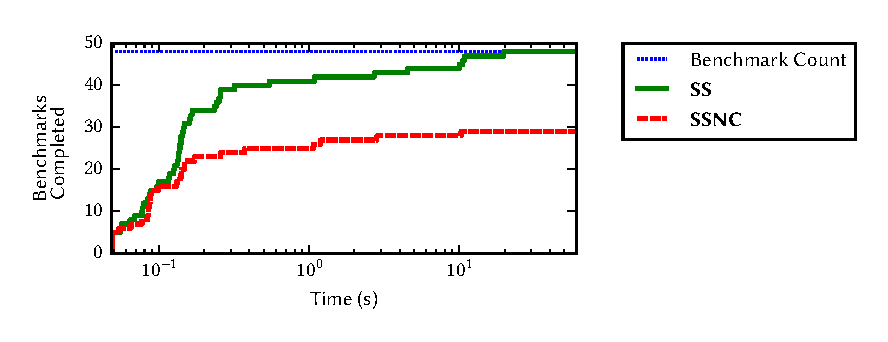
\includegraphics{generated-graphs/times}
  \caption{Number of benchmarks that can be solved by a given algorithm in a
    given amount of time. \SSOpt{} is the full symmetric synthesis algorithm.
    \BSOpt{} is the full bijective lens synthesis algorithm. \SSNCOpt{} is the
    symmetric synthesis algorithm without using a library of existing lenses.
    \BSNCOpt{} is the bijective synthesis algorithm without using a library of
    existing lenses. Our symmetric synthesis algorithm is able to complete all
    benchmarks in our benchmark suite in under 30 seconds, and is able to
    complete a majority of the benchmarks without using compositional
    synthesis.}
  \label{fig:times}
\end{figure}

For each benchmark in our benchmark suite, we ran every mode on it with a
timeout of 30 seconds, and average the result over 5 runs.
Figure~\ref{fig:times} summarizes the results of these tests. We find that our
algorithm is able to synthesize all of the benchmarks in our benchmark suite in
under 30 seconds. Without compositional synthesis, the synthesis algorithm is
able to solve 26 problem instances.

\subsection{Slowdown Compared to Bijective Synthesis}

To compare to the existing bijective synthesis algorithm, we run our symmetric
synthesis algorithm on the original Optician benchmark suite. \afm{8} of these
benchmarks had to be slightly altered with tighter specifications or termination
parameters, as we had to alter the original specifications to generate the
correct lens.

To perform this comparison, we synthesized lenses in 2 modes:

\begin{tabulary}{\linewidth}{rL}
  \SSOpt{}: & We synthesize lenses using our symmetric synthesis algorithm with all optimizations enabled.\\
  \BSOpt{}: & We synthesize lenses using the existing bijective synthesis
              algorithm with all optimizations enabled.\\
\end{tabulary}\\

For each benchmark in our benchmark suite, we ran every mode on it with a
timeout of 30 seconds, and average the result over 5 runs.
Figure~\ref{fig:times_bijective} summarizes the results of these tests. On
average, \SSOpt{} took 2.1 times (\afm{3.5} seconds) longer to complete than
\BSOpt{}.

\begin{figure}
  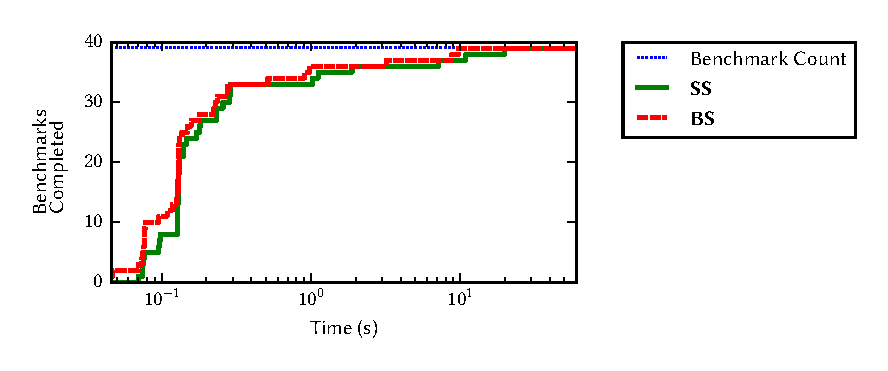
\includegraphics{generated-graphs/times_bijective}
  \caption{Number of benchmarks that can be solved by a given algorithm in a
    given amount of time. \SSOpt{} is the full symmetric synthesis algorithm.
    \BSOpt{} is the full bijective lens synthesis algorithm. \SSNCOpt{} is the
    symmetric synthesis algorithm without using a library of existing lenses.
    \BSNCOpt{} is the bijective synthesis algorithm without using a library of
    existing lenses. Our symmetric synthesis algorithm is able to complete all
    benchmarks in our benchmark suite in under 30 seconds, and is able to
    complete most of the benchmarks without using compositional synthesis.}
  \label{fig:times_bijective}
\end{figure}

The slowest completed benchmark for both synthesis algorithms is
\texttt{xml\_to\_augeas.boom}, a benchmark that converts arbitrary XML up to
depth 3 into a serialized version of the structured dictionary representation
used in Augeas. This benchmark takes 18.9 seconds for the symmetric synthesis
algorithm to complete, and 9.3 seconds the bijective synthesis algorithm to
complete. 

\subsection{The Effects of Our Heuristics}
We evaluate the usefulness of (1) our information theoretic metric, and (2) our
termination heuristic.  To this end, we run our program in 3 different modes:\\
\begin{tabulary}{\linewidth}{rL}
  \AnyOpt{}: & We synthesize any lens that satisfies the specification, with no
               notion of cost.\\
  \FLOpt{}: &  The first time \GreedySynth finds a lens, the synthesis procedure
              returns that lens.\\
  \CCOpt{}: & We replace our information theoretic cost metric with one where
              the cost of the lens is the number of disonnects plus the number
              of merges.\\
  \ZTOpt{}: & \ZTOpt{} runs the algorithm with the termination parameter
    universally set to 0 (default). \\
  \TFTOpt{}: & \TFTOpt{} runs the algorithm with the
    termination parameter universally set to 25. \\
  \NTFTOpt{}: & \NTFTOpt{} runs the algorithm with the
    termination parameter universally set to -25. \\
\end{tabulary}

\begin{figure}
  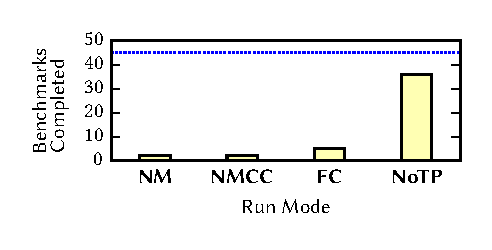
\includegraphics{generated-graphs/metrics_importance}
  \caption{Number of benchmarks that synthesize the correct lens by a given
    algorithm. \AnyOpt{} provides no notion of cost, and merely returns the
    first lens it finds that satisfies the specification. \FLOpt{} provides a
    notion of cost to \GreedySynth, but once a satisfying lens is greedily
    found, that lens is returned. \CCOpt{} synthesizes lenses, where the cost of
    a lens is the number of disconnects plus the number of merges. \ZTOpt{} runs
    the algorithm with the termination parameter universally set to 0 (default).
    \TFTOpt{} runs the algorithm with the termination parameter universally set
    to 25. \NTFTOpt{} runs the algorithm with the termination parameter
    universally set to -25.}
  \label{fig:metric}
\end{figure}

Figure~\ref{fig:metric} summarizes the result of this experiment. We find that
our metrics are very important for finding the correct lens. Our
information-theoretic metric is critical for finding the correct lens. Indeed,
only \afm{10} of our benchmarks succeeded when running in \CCOpt{} mode.

Our termination condition is also quite important. When running in \FLOpt{},
only \afm{5} lenses are found. The first cluster in which a lens is found is
rarely the correct cluster. However, our termination condition is not perfect.
Sometimes users must tell the algorithm to ``keep going'' or ``stop early.''
Without termination parameters, our algorithm finds the correct lens for 36 of
our 45 benchmarks, 9 of them need help in the form of a termination parameter
for finding the correct lens. That being said, our default parameter finds a
good middle-ground. Both \TFTOpt{} and \NTFTOpt{} synthesized the correct lens
less often than \ZTOpt.  \TFTOpt{} necessitates too good a lens, so the search
procedure keeps spinning, and \NTFTOpt{} terminates early, not finding the
correct lens.
% end evaluation

% begin related-work
\section{Related Work}
\label{sec:related}

In this paper, we have designed and implemented a new, pragmatic
formulation of symmetric lenses as well as new program synthesis
techniques.  In this section, we analyze the relationship
between our simple symmetric
lenses and two previous lens languages:  classical symmetric lenses
and asymmetric lenses.  We also comment on related
program synthesis techniques.

\subsection{Relationship with Classical Lens Languages}
\label{sec:relationship}
%\paragraph*{Formalization}
%We have reformulated the problem addressed by classical
%symmetric lenses with simple symmetric lenses.

\paragraph*{Symmetric Lenses}
A classical symmetric lens
$\Lens$ between $X$ and $Y$ consists of 4 components: a complement $C$, a
designated element $init \in C$, and two functions,
$\PutRSym$ and $\PutLSym$, that propagate changes in one format to the other.
\begin{enumerate}
\item $\PutRSym \OfType X \times C \rightarrow Y \times C$
\item $\PutLSym \OfType Y \times C \rightarrow X \times C$
\end{enumerate}
In this formulation, data unique to each side are stored in the complement.
When one format is edited, the \PutR
or \PutL function stitches together the edited data with data
stored in the complement.  The  $init$ element is used as the
initial value of $C$ and specifies default behavior when data is missing.
For instance, to implement the
scenario in Figure~\ref{fig:minimized-representations}, the complement
would consist of a list of pairs of salary and company name.

Classical symmetric lenses satisfy the following equational laws.
\begin{equation}
  \tag{\PutRL}
  \frac{\PutRSymOf{(x,c)} = (y,c'')}{\PutLSymOf{(y,c'''')} = (x,c')}
\end{equation}
\begin{equation}
  \tag{\PutLR}
  \frac{\PutLSymOf{(y,c)} = (x,c')}{\PutRSymOf{(x,c')} = (y,c')}
\end{equation}

Two classical symmetric lenses are equivalent if they output the same
formats given any sequence of edits. Formally, given a lens
$\Lens \in X \leftrightarrow Y$,
an \emph{edit} for $\Lens$ is a member of $X + Y$. Consider
the function $apply$, which, given a lens and an element of that lens's
complement, is a function from sequences of edits to sequences of edits. If
$apply(\Lens,c,es) = es'$, then that means, starting with complement $c$, after
edit $es_i$, the lens $\Lens$ synchronizes the other data to $es'_i$.
\[
  \inferrule
  {
  }
  {
    apply(\Lens,c,[]) = []
  }
\]
\[
  \inferrule
  {
    \Lens.putr(x,c) = (y,c')\\
    apply(\Lens,c',es) = es'
  }
  {
    apply(\Lens,c,(\InLOf{x})::es) = (\InROf{y})::es'
  }
\]
\[
  \inferrule
  {
    \Lens.putl(y,c) = (x,c')\\
    apply(\Lens,c',es) = es'
  }
  {
    apply(\Lens,c,(\InROf{y})::es) = (\InLOf{x})::es'
  }
\]
\noindent
Two lenses, $\Lens_1$ and $\Lens_2$, are equivalent if
$apply(\Lens_1,\Lens_1.init,es) = apply(\Lens_2,\Lens_2.init,es)$ for all edit
sequences $es$.

%% By describing our lenses in this complement style, we can express an incredibly
%% wide class\bcp{where is the evidence that this class of lenses is {\em
%%     usefully} wider than simple symmetric lenses?} of lenses, as these complements permit storing any amount of
%% information in them.  However, they pose problems when implementing them in
%% real-world systems and in synthesizing them.

%\paragraph*{Issues with Classical Symmetric Lenses}
\iffalse
Using symmetric lenses for
synchronization forces us to maintain not just two files that we aim to
sycnrhonize, but three. \bcp{I don't find it unintuitive, and I think we
  should be careful not to oversell the difficulty of storing the
  complements.  It requires more engineering, but it's not rocket
  science.}This is unintuitive, and creates many problems in 
practice. For example, consider the situation where I am synchronizing a crontab
and job manager file. I am synchronizing across computers, so I must either
maintain a copy of the complement on each computer, and keep them synchronized,
or figure out a computer to hold the complement, and make sure all edits go
through that complement. Furthermore, if I want to change the synchronization to
a different computer, I don't need to merely make sure that my files are moved
to the computer, I also have to make sure that I correctly move the complement,
and hook up that complement to be used for that synchronization task. This is a
huge divergence from other synchronization utilities\bcp{No.  For example,
  Unison maintains a database on each replica recording, for each file, what
its hash was after the last time the two replicas were synchronized.}, where all
that needs to be 
done is maintain the files. Using those for synchronization, edits can be sent
over the wire, and the appropriate function can stitch together those edits, no
additional state needed.
\fi
While classical symmetric are more expressive than simple symmetric
lenses, it is unclear whether this additional expressiveness is useful in
practice.  Moreover, classic symmetric lenses come with 
some disadvantages.
For one, an implementation of classical symmetric lenses
would need to squirrel away the complement in
an auxiliary file somwhere, which likely requires more engineering.
However, more significant issues arise in synthesis.
First, because each lens has a custom complement, one can no longer
specify the put functions through input/output examples alone.  One
alternative would be to enrich specifications with edit sequentials;
another would be to specify the structure of complements explicitly
(though the latter would be somewhat akin to specifying the internal
state of a program).  In either case, the complexity of the specifications
increases.
%% addition, users would have to specify some auxilary 
%% to specify the behavior through the observable behavior of edit sequences.
%% Second, there are lenses that require arbitrarily long edit sequences to
%% differentiate between: consider the lens that keeps two formats equal for the
%% first $k$ non-identity edits, then keeps them completely unsynchronized for all
%% future edits.  This requires an edit sequence of $k$ edits to differentiate
%% between this lens and the identity lens.  Simple symmetric lenses avoid this
%% problem by disallowing such lenses: we can't keep track of the number of
%% non-identity edits performed unless there are explicit fields in the data
%% formats keeping track of them.  While we are reducing the expressivity of our
%% lenses with this restriction, we feel the benefits outweigh the costs.

\paragraph*{Relation with Simple Symmetric Lenses} To formalize how simple
symmetric lenses work as synchronization tools, we define an $apply$ function on
them, much like one defines an $apply$ on classical symmetric lenses: Given a
simple symmetric lens and an optional pair of source and target strings, $apply$
is a function from sequences of edits to sequences of edits. If
$apply(\Lens,\None,es) = es'$, then starting with no prior data, after edit
$es_i$, the lens \Lens synchronizes the updates the data in the non-edited
format (the right format if $es_i = \InLOf{x}$, and the left format if $es_i =
\InROf{y}$) to $es_i'$. If $apply(\Lens,\SomeOf{(x,y)},es) = es'$, then that
means, starting with data $x$ and $y$ on the left and right, respectively, after
edit $es_i$, the lens \Lens synchronizes the other data to $es_i'$.

\[
  \inferrule
  {
  }
  {
    apply(\Lens,xyo,[]) = []
  }
\]
\[
  \inferrule
  {
    \Lens.\CreateROf{x} = y\\
    apply(\Lens,\SomeOf{(x,y)},es) = es'
  }
  {
    apply(l,\None,\InLOf{x}::es) = \InROf{y}::es'
  }
\]
\[
  \inferrule
  {
    \Lens.\CreateLOf{y} = x\\
    apply(\Lens,\SomeOf{(x,y)},es) = es'
  }
  {
    apply(l,\None,\InROf{y}::es) = \InLOf{x}::es'
  }
\]
\[
  \inferrule
  {
    \Lens.\PutROf{x'}{y}  = y'\\
    apply(\Lens,\SomeOf{(x',y')},es) = es'
  }
  {
    apply(l,\SomeOf{(x,y)},\InLOf{x'}::es) = \InROf{y'}::es'
  }
\]
\[
  \inferrule
  {
    \Lens.\PutLOf{y'}{x}  = x'\\
    apply(\Lens,\SomeOf{(x',y')},es) = es'
  }
  {
    apply(l,\SomeOf{(x,y)},\InROf{y'}::es) = \InLOf{x'}::es'
  }
\]

We have reformulated symmetric lenses in a style similar to existing asymmetric
lens formulations. However, some symmetric lenses certainly are inexpressible in
the simple symmetric lens formulation. We formalize which are expressible
with a restriction on symmetric lenses. We define \emph{forgetful symmetric
  lenses} to be symmetric lenses that satisfy the following additional laws.
\begin{equation}
  \tag{\ForgetfulRL}
  \begin{mathprooftree}
    \AxiomC{$\Lens.putr(x,c_1) = (\_,c_1')$}
    \def\extraVskip{.5pt}
    \noLine 
    \UnaryInfC{$\Lens.putr(x,c_2) = (\_,c_2')$}
    \AxiomC{$\Lens.putl(y,c_1') = (\_,c_1'')$}
    \def\extraVskip{.5pt}
    \noLine 
    \UnaryInfC{$\Lens.putl(y,c_2') = (\_,c_2'')$}
    \def\extraVskip{2pt}
    \singleLine
    \BinaryInfC{$c_1'' = c_2''$}
  \end{mathprooftree}
\end{equation}
\begin{equation}
  \tag{\ForgetfulLR}
  \begin{mathprooftree}
    \AxiomC{$\Lens.putl(y,c_1) = (\_,c_1')$}
    \def\extraVskip{.5pt}
    \noLine 
    \UnaryInfC{$\Lens.putl(y,c_2) = (\_,c_2')$}
    \AxiomC{$putr(x,c_1') = (\_,c_1'')$}
    \def\extraVskip{.5pt}
    \noLine 
    \UnaryInfC{$\Lens.putr(x,c_2') = (\_,c_2'')$}
    \def\extraVskip{2pt}
    \singleLine
    \BinaryInfC{$c_1'' = c_2''$}
  \end{mathprooftree}
\end{equation}

Intuitively, these equations state that complements are uniquely determined by the most
recently input $x$ and $y$. Hence, such lenses correspond closely \dpw{replace ``closely'' with
``exactly''?} with simple symmetric
lenses, where all state is maintained by the current state of the $x$ and $y$
data. Forgetful symmetric lenses express exactly the same $apply$ function as
simple symmetric lenses.

\begin{theorem}
  Let $\Lens$ be a classical symmetric lens. The lens $\Lens$ is equivalent to a forgetful
  lens if, and only if, there exists a simple symmetric lens $\Lens'$ where
  $apply(\Lens,\Lens.init,es) = apply(\Lens',\None,es)$, for all put sequences $es$.
\end{theorem}

\bcp{I guess we could also show that equivalence of simple symmetric lenses
  is just the identity relation?}
\sam{No; for example the identity lens of a concatenation of two regular
  expressions is the same as concatenating the two identity lenses on the
  respective regular expressions}
\afm{I think Benjamin likely means identity relation on the semantic meaning of
  the lenses, which is true.  Would this be a useful thing to prove? It's a 2
  liner.}

\paragraph*{Asymmetric Lenses}
Formally, an {\em asymmetric lens} $ \ell : S \Leftrightarrow V$ is a triple of functions $\ell.\get : S \longrightarrow V$, $\ell.\pput : V \longrightarrow S \longrightarrow S$ and $\ell.\create : V \longrightarrow S$ satisfying the following laws \cite{Focal2005-long2}:
\begin{align*}
\ell.\get \; (\ell.\pput \; s \; v) &= v \tag{PUTGET}\\
\ell.\pput \; s \; (\ell.\get \; s) &= s \tag{GETPUT}\\
\ell.\get \; (\ell.\create \; v) &= v \tag{CREATEGET}
\end{align*}
Despite being less expressive than symmetric lenses, simple symmetric lenses are
strictly more expressive than classical asymmetric lenses.

\begin{theorem}
  Let $\Lens$ be an asymmetric lens. $\Lens$ is also a simple symmetric lens,
  where
  \begin{center}
    \begin{tabular}{rcl}
      $\Lens.\CreateROf{x}$ & $=$ & $\Lens.get \App x$\\
      $\Lens.\CreateLOf{y}$ & $=$ & $\Lens.create \App y$\\
      $\Lens.\PutROf{x}{y}$ & $=$ & $\Lens.get \App x$\\
      $\Lens.\PutLOf{y}{x}$ & $=$ & $\Lens.put \App y \App x$
    \end{tabular}
  \end{center}
\end{theorem}

\subsection{Data Transformation Synthesis}
Over the past decade, the programming languages community has explored
the synthesis of programs from a wide variety of angles.  One of
the key ideas is typically to narrow the program search space by focusing
on a specific domain, and imposing constraints on syntax~\cite{sygus} or
typing~\cite{augustsson-2004,gvero-pldi-2013,osera+:pldi15,feser-pldi-2015,scherer-icfp-2015,frankle+:popl16}, or both.
%, and as has been advocated
%more generally under the rubric of syntax-guided synthesis~\cite{sygus}.

Automation of string transformations, in particular, has been the focus
of much prior attention.  For example, Gulwani and others work on FlashFill
generates one-way spreadsheet transformations from input/output
examples~\cite{flashfill,le-pldi-2014}.  On the one hand,
FlashFill is easier to use because one need not specify the type of
the data being transformed.  On the other hand, this type information
makes it possible to transform more complex formats---Flash Fill
does not synthesize programs with nested loops, for instance,
and hence is incapable of synthesizing the majority of our
benchmarks, even in one direction~\cite{flashfill}.
%% Flashfill, designed
%% for transformation of the cells of spreadsheets, does not scale to
%% more complex formats
%% While this provides an easier
%% interaction model with the user than this work, it requires the algorithm to
%% learn the data formats from the examples. This makes the task much more
%% difficult for the synthesis algorithm, particularly in addressing iterations and
%% disjunctions. Prior work has shown that learning from examples and data format
%% descriptions enables synthesis of much more complex transformations than are
%% permitted by examples alone. Recent work has gone into making these algorithms
%% more robust by delaying the selection of program until seeing what further
%% inputs the program is run on~\cite{?}. By doing this, the synthesis algorithm
%% can learn additional information about the formats from the use of the program.

All pragmatic synthesis algorithms use heuristics of one kind or another.  One of the
goals of the current paper is to try to ground those heuristics in a broader theory,
information theory,
with the hope that this theory may inform future design decisions and help us understand
heuristics crafted in other tools and possibly in other domains.  For instance, we
speculate that some of the heuristics used in
FlashFill (to take one well-documented example) may be connected to some of the principles
laid out here.  For instance, FlashFill prioritizes the substring constructor over the
constant string constructor when ranking possible programs. Such a choice may be understood
in information-theoretic terms as the translation from target back to source would require
more information.  Said another way, our information theoretic metrics measure injectivity
(in both directions, in our case, to measure bijectivity) but applied in one direction, as
is the case for FlashFill, would avoid the highly injective constant functions.  Beyond
constants, another FlashFill heuristic prefers ``wider'' character classes (or token classes)
over ``narrower'' ones.  Selecting a wider set of strings to copy from left-to-right, viewed
in the reverse direction, from right-to-left, results in a function that is closer to being
injective, as measured by information theory.  These are just a few of the heuristics used
in Flashfill; more research would be required (and public disclosure of the details necessary)
to understand the connections fully.

%% In many of these synthesis algorithms the correct transformation is chosen by
%% principals like ``minimize constants''~\cite{?,?,?} and ``most specific
%% generalization''~\cite{?,?,?}. We are the first work to our knowledge to use an
%% information-theoretic measure for finding the correct transformation. However,
%% much of our metrics are compatible with existing metrics: avoiding \Disconnect
%% lenses minimizes constants and creates more specfic transformations (\Disconnect
%% lenses permit more synchronized data).

As discussed in the introduction,
the Optician tool~\cite{optician,maina+:quotient-synthesis} was a building block for
our work.  Optician synthesized bijective transformations~\cite{optician} and
bijections modulo quotients~\cite{maina+:quotient-synthesis}, but could
not synthesize more complex bidirectional transformations where one format contains
important information not present in the other---a common situation in the real
world.  From a technical perspective, the first key novelty in our work involves the definition, theory,
analysis, and implementation of a new class of simple symmetric lenses, designed
for synthesis.  The second key technical innovation involves the use of stochastic
regular expressions and information theory to guide the search for program transformations.
As mentioned earlier, we believe such information theoretic techniques may have broad utility
in helping us understand how to formulate a search for a data transformation function.
%% The central contributions
%% only synchronized transformations between formats in
%% bijective correspondence, but few formats satisfy that constraint. Recent
%% enhancements have permitted synthesis of more expressive lenses, quotient
%% bijective lenses. These enhancements were made by strengthening the
%% specifications from regular expressions to QREs, regular expressions annotated
%% with information on normal forms of the language. This enhancement permits
%% synthesizing transformations between formats whose normal forms are in bijective
%% correspondence. While we have not integrated our system to permit QRE
%% specifications, we see no reason the two systems cannot be integrated.

While our tool uses types and examples to specify invertable transformations, other
tools have been shown to synthesize a backwards transformation from ordinary code designed
to implement the forwards transformation.  For instance, Hu and
D'Antoni~\cite{program-inversion-symbolic-transducers} show how to invert transformations
using symbolic finite automata, and
Voigtl\"{a}nder~\cite{bidirectionalization-for-free} demonstrates how to
construct reverse transformations from forwards transformations
by exploiting parametricity properties.  These kinds of tools are very useful, but in different
circumstances from ours (namely, when one already has the code to implement one direction of
the transformation).

More broadly, information theory and probabilistic languages are common tools
in natural language understanding,  machine translation, information retrieval,
data extraction and grammatical inference (see Pereira~\cite{pereira:info-theory},
for an introduction).  Indeed, our work was inspired, in part, by the PADS format
inference tool~\cite{pads:synthesis}, which was in turn inspired by earlier work on
probabilistic gramatical inference
and information extraction~\cite{kushmerick-thesis,arasu:extracting}.  More specifically, PADS
used an information-theoretic metric to help judge the quality of inferred grammars
for ad hoc data formats.  However, PADS did not synthesize data transformers, and
we are not aware of the use of information-theoretic principles in type-directed or syntax-guided
synthesis of DSL programs. 

%% Other work synthesizing invertible transformations was done by inverting a
%% previously defined transformation.  This has been done by exploiting
%% parametricity to invert transformations~\cite{}, and by inverting symbolic
%% finite automata~\cite{?}.

%% \subsection{Type-Directed Synthesis}

%% Type-directed synthesis uses type information to tighten specifications and
%% reduce the number of possible programs. Typically, type-directed synthesis
%% techniques use the types to orient the search space.  Our work interestingly
%% deals with types with many semantic equivalences on them. InSynth~\cite{?}
%% deals with the same problem when trying to synthesize transformations involving
%% library functions. InSynth addresses this in a similar manner to this work: by
%% normalizing the types we don't need to search through the equivalences on those
%% types.

% end related-work

% begin conclusion
\section{Conclusion}
\label{sec:conc}
We have developed a synthesis algorithm for synthesizing synchronization
functions between data formats that may not be in bijective correspondence. We
do this by synthesizing symmetric lenses. However, existing symmetric lens
formulations use complex complements to store external state. We identify a
restriction on symmetric lenses, simple symmetric lenses. We develop combinators
for simple symmetric lenses on string data. We show how to synthesize these
lenses from regular expression specifications. Prior work could return
\emph{any} satisfying lens, as the type system was restrictive enough that any
satisfying lens would typically be the correct satisfying lens. Because of the
increased flexibility of the symmetric lens language, we identify an
information-theoretic heuristic for finding a likely satisfying lens. We
developed a greedy synthesis algorithm that aims to find the lens of lowest
cost. We demonstrate empiraclly that our algorithm can find lenses quickly, and
our heuristic makes finding the correct lens require fewer specifications.

% end conclusion

% begin acknowledgements
\begin{acks}
\end{acks}
% end acknowledgements

\ifanon\else
\fi

% We recommend abbrvnat bibliography style.

% The bibliography should be embedded for final submission.

\bibliography{local,bcp}

\appendix

\ifappendices

\onecolumn


\paragraph*{Symmetric DNF Lenses: Typing and Semantics}
The typing judgment is a 3-ary relation over a single DNF lens, and two DNF
regular expressions. If $\SDNFLens \OfType \DNFRegex \Leftrightarrow
\DNFRegexAlt$, then the $\SDNFLens.\CreateR$, $\SDNFLens.\CreateL$,
$\SDNFLens.\PutR$, and $\SDNFLens.\PutL$ functions form a symmetric lens.

The typing judgement has 3 components. The first is the sublens components,
confirming that the sequence lenses the DNF lens is comprised of are all
well-typed. The second guarantees that if each sequence on the left has a
sequence lens that can be used for \CreateR{}s and \PutR{}s. The last guarantees
the same for sequences on the right, with \CreateL{} and \PutL{}.

\[
  \inferrule*
  {
    \SSQLens_1 \OfType \Sequence_{i_1} \Leftrightarrow \SequenceAlt_{j_1}\\
    \ldots\\
    \SSQLens_p \OfType \Sequence_{i_p} \Leftrightarrow \SequenceAlt_{j_p}\\\\
    i_{c_1} = 1\\
    \ldots\\
    i_{c_q} = q\\\\
    j_{d_1} = 1\\
    \ldots\\
    j_{d_r} = r
  }
  {
    (\SDNFLensOf{(i_1,j_1,\SSQLens_1)\DNFLSep
      \ldots\DNFLSep
      (i_p,j_p,\SSQLens_p)}
    ,\ListOf{c_1;\ldots;c_q}
    ,\ListOf{d_1;\ldots;d_r})
    \OfType\\\\
    \DNFOf{(\Sequence_1,\Probability_1) \DNFSep \ldots \DNFSep (\Sequence_q,\Probability_q)}
    \Leftrightarrow
    \DNFOf{(\SequenceAlt_1,\ProbabilityAlt_1) \DNFSep \ldots \DNFSep (\SequenceAlt_r,\ProbabilityAlt_q)}
  }
\]

The \CreateR{} function looks for the sequence the provided string matches. If
the string matches sequence $\Sequence_x$, then the lens will look in the create
list at position $x$ to find which sequence lens to use. Then, the sequence lens
transforms the given string using that sequence lens.

The \PutR{} function finds what pairs sequences the input source and view
strings match.  If there that pair of sequences have a sequence lens between
them, then the DNF lens merely performs that sequence lens on the provided
strings.  If there isn't a pair of sequence lenses between them, then \CreateR{}
is performed on the source, with the view forgotten.

The \CreateL{} and \PutL{} functions are defined symmetrically.

\begin{tabular}{@{}r@{\ }c@{\ }l@{}}
  $\CreateR{} \App s$ & = & $\SSQLens_{c_x}.\CreateR{} \App s$ if $s \in \Sequence_x$\\
  $\CreateL{} \App v$ & = & $\SSQLens_{d_y}.\CreateL{} \App v$ if $v \in \SequenceAlt_y$\\
  $\PutR{} \App s \App v$ & = &
                               $\begin{cases*}
                                 \SSQLens_x.\PutR{} \App s \App v & if $s \in \Sequence_{i_x}$ and $v \in \SequenceAlt_{j_x}$\\
                                 \CreateR{} \App s & if $\nexists x.$ $s \in \Sequence_{i_x}$ and $v \in \SequenceAlt_{j_x}$
                               \end{cases*}$\\
  $\PutL{} \App v \App s$ & = &
                               $\begin{cases*}
                                 \SSQLens_y.\PutL{} \App v \App s & if $v \in \SequenceAlt_{j_y}$ and $s \in \Sequence_{i_y}$\\
                                 \CreateL{} \App v & if $\nexists y.$ $v \in \SequenceAlt_{j_y}$ and $s \in \Sequence_{i_y}$
                               \end{cases*}$
\end{tabular}

\paragraph*{Symmetric Sequence Lenses: Typing and Semantics}
The typing judgment is a 3-ary relation over a single Sequence lens, and two
sequences. If $\SSQLens \OfType \Sequence \Leftrightarrow \SequenceAlt$, then
the $\SSQLens.\CreateR$, $\SSQLens.\CreateL$, $\SSQLens.\PutR$, and
$\SSQLens.\PutL$ functions form a symmetric lens.

The typing judgement has 4 components. The first is the sublens components,
confirming that the atom lenses the sequence lens is comprised of all are
well-typed. The second guarantees that if each string that will be used for
\CreateR{}s are members of the correct atoms.  The third guarantees
the same for strings and atoms on the right, with \CreateL.  The last guarantees
that each atom is mapped by at most one atom lens.

\[
  \inferrule*
  {
    \SAtomLens_1 \OfType \Atom_{i_1} \Leftrightarrow \AtomAlt_{j_1}\\
    \ldots\\
    \SAtomLens_p \OfType \Atom_{i_p} \Leftrightarrow \AtomAlt_{j_p}\\\\
    \String_1 \in \Atom_1\\
    \ldots\\
    \String_q \in \Atom_q\\\\
    \StringAlt_1 \in \AtomAlt_1\\
    \ldots\\
    \StringAlt_r \in \AtomAlt_r\\\\
    i_x = i_y \BooleanImplies x = y\\
    j_x = j_y \BooleanImplies x = y
  }
  {
    (\SSQLensOf{(i_1,j_1,\SAtomLens_1)\SeqLSep
      \ldots\SeqLSep
      (i_p,j_p,\SAtomLens_p)}
    ,\ListOf{\String_1;\ldots;\String_q}
    ,\ListOf{\StringAlt_1;\ldots;\StringAlt_r})\\
    \OfType
    \SequenceOf{\String_0'''' \SeqSep \Atom_1 \SeqSep \ldots \SeqSep \Atom_q
      \SeqSep \String_q'}
    \Leftrightarrow
    \SequenceOf{\StringAlt_0' \SeqSep \AtomAlt_1 \SeqSep \ldots \SeqSep \AtomAlt_r \SeqSep \StringAlt_r'}
  }
\]

For each component of the string matching an atom, the \CreateR function looks
for the atom lens that maps on the atom. If there is such an atom lens,
\SAtomLens, then that the sequence lens puts the provided string into the
default string for the target atom. If there is no such atom lens, then the
sequence lens merely uses the default string.

For each component of the string matching an atom, the \PutR function looks
for the atom lens that maps on the atom. If there is such an atom lens,
\SAtomLens, then that the atom lens puts the provided string of the source atom into the
string of the target atom. If there is no such atom lens, then the
sequence lens merely recovers the target's string.

The \CreateL{} and \PutL{} functions are defined symmetrically.

\begin{tabular}{@{}r@{\ }c@{\ }l@{}}
  $\CreateR{} \App \String_0'\Concat \String_1'' \Concat \ldots \Concat \String_q'' \Concat \String_q'$
  & = 
  & $\StringAlt_0' \Concat \StringAlt_1'' \Concat \ldots \Concat
    \StringAlt_r'' \Concat \StringAlt_r'$\\
  & & where $\StringAlt_y'' =
    \begin{cases*}
      \SAtomLens_k.\PutROf{\String_{i_k}''}{\StringAlt_y} & if $j_k = y$\\
      \StringAlt_y & if $\nexists k. j_k = y$\\
    \end{cases*}$\\
  $\CreateL{} \App \StringAlt_0'\Concat \StringAlt_1'' \Concat \ldots \Concat \StringAlt_q''
  \Concat \StringAlt_q'$
  & = 
  & $\String_0' \Concat \String_1'' \Concat \ldots \Concat
    \String_r'' \Concat \String_r'$\\
  & & where $\String_x'' =
    \begin{cases*}
      \SAtomLens_k.\PutROf{\StringAlt_{j_k}''}{\String_x} & if $i_k = x$\\
      \String_x & if $\nexists k. i_k = x$\\
    \end{cases*}$\\
  $\PutR{} \App (\String_0'\Concat \String_1'' \Concat \ldots \Concat \String_q'' \Concat \String_q') \App (\StringAlt_0'\Concat \StringAlt_1'' \Concat \ldots \Concat \StringAlt_q'' \Concat \StringAlt_q')$
  & =
  & $\StringAlt_0'\Concat \StringAlt_1''' \Concat \ldots \Concat \StringAlt_q''' \Concat \StringAlt_q'$\\
  & & where
      $t_y''' =
      \begin{cases*}
        \SAtomLens_k.\PutROf{\String_{i_k}''}{\StringAlt_{y}''} & if $j_k = y$\\
        \StringAlt_y'' & if $\nexists k. j_k = y$\\
      \end{cases*}$\\
  $\PutL{} \App (\StringAlt_0'\Concat \StringAlt_1'' \Concat \ldots \Concat \StringAlt_q'') \Concat (\StringAlt_q' \App \String_0'\Concat \String_1'' \Concat \ldots \Concat \String_q'' \Concat \String_q')$
  & =
  & $\String_0'\Concat \String_1''' \Concat \ldots \Concat \String_r''' \Concat \String_r'$\\
  & & where
      $s_x''' =
      \begin{cases*}
        \SAtomLens_k.\PutLOf{\StringAlt_{j_k}''}{\String_{x}''} & if $i_k = x$\\
        \String_x'' & if $\nexists k. i_k = x$\\
      \end{cases*}$\\
\end{tabular}

\paragraph*{Symmetric Atom Lenses: Typing and Semantics}
The typing judgment is a 3-ary relation over a single atom lens, and two
atoms. If $\SAtomLens \OfType \Atom \Leftrightarrow \AtomAlt$, then
the $\SAtomLens.\CreateR$, $\SAtomLens.\CreateL$, $\SAtomLens.\PutR$, and
$\SAtomLens.\PutL$ functions form a symmetric lens.

The typing judgement just confirms that the DNF lens that comprises the
sequence lens is also well typed.

\[
  \inferrule*
  {
    \SDNFLens \OfType \DNFRegex \Leftrightarrow \DNFRegexAlt
  }
  {
    \StarOf{\SDNFLens}
    \OfType \PRegexStar{\DNFRegex}{\Probability}
    \Leftrightarrow \PRegexStar{\DNFRegexAlt}{\ProbabilityAlt}
  }
\]

For each component of the string matching an atom, the \CreateR function looks
for the atom lens that maps on the atom. If there is such an atom lens,
\SAtomLens, then that the sequence lens puts the provided string into the
default string for the target atom. If there is no such atom lens, then the
sequence lens merely uses the default string.

For each component of the string matching an atom, the \PutR function looks
for the atom lens that maps on the atom. If there is such an atom lens,
\SAtomLens, then that the atom lens puts the provided string of the source atom into the
string of the target atom. If there is no such atom lens, then the
sequence lens merely recovers the target's string.

The \CreateL{} and \PutL{} functions are defined symmetrically.

\begin{tabular}{@{}r@{\ }c@{\ }l@{}}
  $\CreateR{} \App \String_0 \Concat \ldots \Concat \String_n$
  & = 
  & $\StringAlt_1 \Concat \ldots \Concat \StringAlt_n$
  where $\StringAlt_i = \SDNFLens.\CreateR \App \String_i$\\
  $\CreateL{} \App \StringAlt_0 \Concat \ldots \Concat \StringAlt_m$
  & = 
  & $\String_1 \Concat \ldots \Concat \String_m$
  where $\String_i = \SDNFLens.\CreateL \App \StringAlt_i$\\
  $\PutR{} \App (\String_0 \Concat \ldots \Concat \String_n) \App
  (\StringAlt_1 \Concat \ldots \Concat \StringAlt_m)$
  & = 
  & $\StringAlt_1' \Concat \ldots \Concat \StringAlt_n'$
    where $\StringAlt_i' =
    \begin{cases*}
      \SDNFLens.\PutR \App \String_i \App \StringAlt_i & if $i \leq m$\\
      \SDNFLens.\CreateR \App \String_i & otherwise
    \end{cases*}$\\
  $\PutL{} \App (\StringAlt_1 \Concat \ldots \Concat \StringAlt_m) \App
  (\String_0 \Concat \ldots \Concat \String_n)$
  & = 
  & $\String_1' \Concat \ldots \Concat \String_m'$
    where $\String_i' =
    \begin{cases*}
      \SDNFLens.\PutL \App \StringAlt_i \App \String_i & if $i \leq n$\\
      \SDNFLens.\CreateL \App \StringAlt_i & otherwise
    \end{cases*}$\\
\end{tabular}


\section{Forgetful Symmetric Lenses}

\begin{property}[Starting Forgetfulness RL]
  \label{prop:forget-rl}
  Let $\Lens$ be a forgetful symmetric lens.  If $(x_1',c_1') = \Lens.\PutL \App
  (y,\Snd \App (\Lens.\PutR \App (x,c_1)))$, and
  $(x_2',c_2') = \Lens.\PutL \App
  (y,\Snd \App (\Lens.\PutR \App (x,c_2)))$, then $x_1' = x_2'$.
\end{property}
\begin{proof}
  By \ForgetfulRL, $c_1' = c_2'$. We know $(y,c_1') = \Lens.\PutR \App
  (x_1',c_1')$ and $(y,c_1') = \Lens.\PutR \App (x_2',c_1')$ by \PutLR. By
  \PutRL, we know $(x_1' = \Lens.\PutL \App (y,c_1'))$ and $(x_2' = \Lens.\PutL
  \App (y,c_1')))$. Therefore, by transitivity of equality, $x_1' = x_2'$.
\end{proof}

\begin{property}[Starting Forgetfulness LR]
  \label{prop:forget-lr}
  Let $\Lens$ be a forgetful symmetric lens.  If $(y_1',c_1') = \Lens.\PutR \App
  (x,\Snd \App (\Lens.\PutL \App (y,c_1)))$, and
  $(x_2',c_2') = \Lens.\PutL \App
  (x,\Snd \App (\Lens.\PutR \App (y,c_2)))$,
  then $x_1' = x_2'$.
\end{property}
\begin{proof}
  Symmetric to Starting Forgetfulness RL.
\end{proof}

\begin{definition}[S]
  Let $\Lens$ be a forgetful lens.

  Consider the following four functions $S(\Lens)$, that we wish to satisfy the
  simple symmetric lens laws.

  \begin{centering}
    \begin{tabular}{@{}r@{\ }c@{\ }l@{}}
      $\CreateR{} \App s$
      & =
      & $\Fst \App (\Lens.\PutR{} \App (s,\Lens.init))$\\
      
      $\CreateL{} \App v$
      & =
      & $\Fst \App (\Lens.\PutL{} \App (v,\Lens.init))$\\
      
      $\PutR{} \App s \App v$
      & =
      & $\LetIn{(\_,c)}{\Lens.\PutL \App (v,\Lens.init)}$\\
      &
      & $\LetIn{(s',\_)}{\Lens.\PutR \App (s,c)}$\\
      &
      & $s'$\\
      
      $\PutL{} \App v \App s$
      & =
      & $\LetIn{(\_,c)}{\Lens.\PutR \App (s,\Lens.init)}$\\
      &
      & $\LetIn{(y',\_)}{\Lens.\PutL \App (v,c)}$\\
      &
      & $y'$\\
    \end{tabular}
  \end{centering}
\end{definition}

\begin{mylemma}
  If $\Lens$ is a forgetful symmetric lens, then $S(\Lens)$ is a simple symmetric
  lens.
\end{mylemma}
\begin{proof}
  
  \CreatePutRL{}:
  
  \begin{centering}
    \begin{tabular}{@{}r@{\ }c@{\ }l@{\ }l}
      $S(\Lens).\PutLOf{(S(\Lens).\CreateROf{x})}{x}$
      & =
      & $S(\Lens).\PutLOf{(\Fst \App (\Lens.\PutR{(x,\Lens.init)}))}{x}$
      & By unfolding definitions
      \\
      
      & =
      & $\LetIn{(\_,c)}{\Lens.\PutR \App (x,\Lens.init)}$\\
      &
      & $\LetIn{(y',\_)}{\Lens.\PutL \App (\Fst \App (\Lens.\PutR{(x,\Lens.init)}),c)}$\\
      &
      & $y'$
      & By unfolding definitions\\
      
      & =
      & $\LetIn{(y',\_)}{\Lens.\PutL \App (\Lens.\PutR \App (x,\Lens.init))}$\\
      &
      & $y'$
      & By tuple harmony \\
      
      & =
      & $x$
      & By \PutRL \\
    \end{tabular}
  \end{centering}

  \CreatePutLR{}:  Symmetric to \CreatePutRL{}

  \PutRL{}:

  \begin{centering}
    \begin{tabular}{@{}r@{\ }c@{\ }l@{\ }l}
      $S(\Lens).\PutLOf{(S(\Lens).\PutROf{x}{y})}{x}$
      & =
      & $\LetIn{(\_,c)}{\Lens.\PutL \App (y,\Lens.init)}$\\
      & & $\LetIn{(y',c')}{\Lens.\PutR \App (x,c)}$\\
      & & $S(\Lens).\PutLOf{y'}{x}$
      & By unfolding definitions
      \\
      
      & =
      & $\LetIn{(\_,c)}{\Lens.\PutL \App (y,\Lens.init)}$\\
      & & $\LetIn{(y',c')}{\Lens.\PutR \App (x,c)}$\\
      & & $\LetIn{(\_,c'')}{\Lens.\PutR \App (x,\Lens.init)}$\\
      & & $\LetIn{(x',c''')}{\Lens.\PutL \App (y',c'')}$\\
      & & $x'$
      & By unfolding definitions
    \end{tabular}
  \end{centering}

  At this point, we know from \PutRL that $(x,c') = \Lens.\PutL \App (y',c')$.
  By Property~\ref{prop:forget-rl}, this means that $x' = x$, as desired.

  \PutLR{}:  Symmetric to \PutRL{}
\end{proof}

\begin{definition}
  Fix a symmetric lens $\Lens$ beteween $X$ and $Y$. Consider the
  function, $\SingleApp_{\Lens} \OfType (X + Y) \times \Lens.C
  \rightarrow ((X + Y) \times \Lens.C)$, defined as:

  \begin{tabular}{@{}r@{\ }c@{\ }l@{\ }l}
    $\SingleApp_{\Lens}(\InLOf{x},c)$
    & =
    & $\LetIn{(y,c')}{\Lens.\PutRSymOf{(x,c)}}$\\
    &
    & $(\InROf{y},c')$\\
    
    $\SingleApp_{\Lens}(\InROf{y},c)$
    & =
    & $\LetIn{(x,c')}{\Lens.\PutLSymOf{(y,c)}}$\\
    &
    & $(\InLOf{x},\SomeOf{(x,y)})$
  \end{tabular}
\end{definition}

\begin{definition}
  Fix a simple symmetric lens $\Lens$ beteween $X$ and $Y$. Consider the
  function, $\SingleApp_{\Lens} \OfType ((X + Y) \times \OptionOf{(X \times Y)})
  \rightarrow ((X + Y) \times \OptionOf{(X \times Y)})$, defined as:

  \begin{tabular}{@{}r@{\ }c@{\ }l@{\ }l}
    $\SingleApp_{\Lens}(\InLOf{x},\None)$
    & =
    & $\LetIn{y}{\Lens.\CreateROf{x}}$\\
    &
    & $(\InROf{y},\SomeOf{(x,y)})$\\
    
    $\SingleApp_{\Lens}(\InROf{y},\None)$
    & =
    & $\LetIn{x}{\Lens.\CreateLOf{y}}$\\
    &
    & $(\InLOf{x},\SomeOf{(x,y)})$\\
    
    $\SingleApp_{\Lens}(\InLOf{x'},\SomeOf{(x,y)})$
    & =
    & $\LetIn{y'}{\Lens.\PutROf{x'}{y}}$\\
    &
    & $(\InROf{y'},\SomeOf{(x',y')})$\\
    
    $\SingleApp_{\Lens}(\InROf{y'},\SomeOf{(x,y)})$
    & =
    & $\LetIn{x'}{\Lens.\PutLOf{y'}{x}}$\\
    &
    & $(\InROf{x'},\SomeOf{(x',y')})$\\
  \end{tabular}
\end{definition}

\begin{definition}
  Fix a symmetric lens \Lens over $X$ and $Y$. We define the relation $R_\Lens$
  over $\Lens.C$ and $\OptionOf{(X \times Y)}$ as the largest relation such
  that:
  \begin{enumerate}
  \item $R_\Lens(c,None) \BooleanImplies c = \Lens.init$
  \item $R_\Lens(c,Some (x,y)) \BooleanImplies
    \Lens.\PutRSymOf{(x,c)} = (y,c) \BooleanAnd
    \Lens.\PutLSymOf{(y,c)} = (x,c)$
  \end{enumerate}
\end{definition}

\begin{mylemma}
  \label{lem:s-equiv}
  Let $\Lens$ be a symmetric lens.  Let $c \in \Lens.C$ be a complement, and
  $xyo \in \OptionOf{(X \times Y)}$.  If $R_{\Lens}(c,xyo)$, then
  $apply(\Lens,c,es) = apply(S(\Lens),xyo,es)$.
\end{mylemma}
\begin{proof}
  By induction on the derivation the application of $apply(S(\Lens),xyo,es)$
  \begin{case}[empty list]
    So by the case, $apply(S(\Lens),xyo,[]) = []$. Furthermore,
    $apply(\Lens,c,[]) = []$, as desired.
  \end{case}
  \begin{case}[first edit is a create right]
    So by the case, $apply(S(l),\None,\InLOf{x}::es) = \InROf{y}::es'$, where
    $S(\Lens).\CreateROf{x} = y$ and $apply(S(\Lens),\SomeOf{(x,y)},es) = es'$.

    As $R_{\Lens}(None,c)$, $c = \Lens.init$. So, performing $apply$ on
    $\Lens.init$, we get $apply(\Lens,\Lens.init,(\InLOf{x})::es) =
    (\InROf{y'})::es''$ where $\Lens.putr(x,c) = (y',c')$ and $apply(\Lens,c',es)
    = es'$.

    So, by definition, $S(\Lens).\CreateROf{x} = \Fst \App (\Lens.\PutRSymOf{(x,\Lens.init)})$, so $y = y'$.

    Furthermore, by \PutRL, $\Lens.\PutLSymOf{(y,c')} = (x,c')$, and by another
    application of \PutLR, $\Lens.\PutRSymOf{(x,c')} = (y,c')$.  This means
    that $R_{\Lens}(c',Some (x,y))$.

    So, by induction assumption, $apply(\Lens,c',es) = apply(S(\Lens),xyo,es)$, so
    $es' = es''$.  This means, $apply(S(l),\None,\InLOf{x}::es) =
    \InROf{y}::es'$ and $apply(\Lens,\Lens.init,(\InLOf{x})::es) =
    (\InROf{y})::es'$, so they are equal, as desired.
  \end{case}
  \begin{case}[first edit is a create left]
    Symmetric to previous case
  \end{case}
  \begin{case}[first edit is a put right]
    So by the case, $apply(S(\Lens),\SomeOf{(x,y)},\InLOf{x'}::es) = \InROf{y'}::es'$, where
    $S(\Lens).\PutROf{x}{y} = y'$ and $apply(S(\Lens),\SomeOf{(x',y')},es) = es'$.

    Performing $apply$ on $c$, we get $apply(\Lens,c,(\InLOf{x'})::es) =
    (\InROf{y'})::es''$ where $\Lens.\PutRSymOf{(x',c)} = (y',c')$ and
    $apply(\Lens,c',es) = es''$.

    So, by definition, $S(\Lens).\PutROf{x}{y} = \Fst \App (\Lens.\PutRSymOf{(x,c'')})$, where $c'' = \Snd \App (\Lens.\PutLSymOf{(y,\Lens.init)})$.

    By assumption, $R_{\Lens}(c,\SomeOf{(x,y)})$, so $\Lens.\PutLSymOf{(y,c)}
    = (x,c)$.  So, by Property~\ref{prop:forget-lr}, we know $y' = y''$.

    Furthermore, by \PutRL, $\Lens.\PutLSymOf{(y',c')} = (x',c')$, and by another
    application of \PutLR, $\Lens.\PutRSymOf{(x',c')} = (y',c')$.  This means
    that $R_{\Lens}(c',Some (x',y'))$.

    So, by induction assumption, $apply(\Lens,c',es) = apply(S(\Lens),xyo,es)$, so
    $es' = es''$.  This means, $apply(S(l),\SomeOf{(x,y)},\InLOf{x'}::es) =
    \InROf{y'}::es'$ and $apply(\Lens,c,(\InLOf{x'})::es) =
    (\InROf{y'})::es'$, so they are equal, as desired.
  \end{case}
  \begin{case}[first edit is a put left]
    Symmetric to previous case
  \end{case}
\end{proof}

\begin{definition}[F]
  Let $\Lens$ be a simple symmetric lens between $X$ and $Y$.

  Consider the following set $C$, distinguished element of that set, $init$, and
  pair of functions $\PutRSym$ and $\PutLSym$, that we wish to satisfy the
  symmetric lens laws, and that we also wish to be forgetful.

  \begin{centering}
    \begin{tabular}{@{}r@{\ }c@{\ }l@{}}
      $C$
      & =
      & $\OptionOf{(X \times Y)}$\\
      
      $init$
      & =
      & $\None$\\
      
      $\PutRSymOf{(x,c)}$
      & =
      & $(y,\SomeOf{(x,y)})$ where $y = \begin{cases*}
        \Lens.\CreateROf{x} & if $c = \None$\\
        \Lens.\PutROf{x}{y'} & if $c = \SomeOf{(x',y')}$\\
        \end{cases*}$\\
      
      $\PutLSymOf{(y,c)}$
      & =
      & $(x,\SomeOf{(x,y)})$ where $x = \begin{cases*}
        \Lens.\CreateLOf{y} & if $c = \None$\\
        \Lens.\PutLOf{y}{x'} & if $c = \Some{(x',y')}$\\
        \end{cases*}$\\
    \end{tabular}
  \end{centering}
\end{definition}

\begin{mylemma}
  \label{lem:f-sym}
  If $\Lens$ is a simple symmetric lens, then $F(\Lens)$ is a symmetric lens.
\end{mylemma}
\begin{proof}
  \PutRL: There are two cases, $c = \None$, and $c = \SomeOf{(x,y)}$.

  \begin{case}[c = \None]
    Let $(y',c') = F(\Lens).\PutRSymOf{(x',\None)}$. This means that $y' =
    \Lens.\CreateROf{x'}$, and $c' = \SomeOf{(x',y')}$.
    
    Now, consider $(x'',c'') = F(\Lens).\PutLSymOf{(y',\SomeOf{(x',y')})}$. By
    unfolding definitions, $x'' = \Lens.\PutLOf{y'}{x'}$. By \CreatePutRL, $x''
    = x'$, meaning $c'' = \SomeOf{(x',y')}$. This means $(x',c') =
    F(\Lens).\PutLSymOf{(y',\SomeOf{(x',y')})}$, as desired.
  \end{case}

  \begin{case}[c = \SomeOf{(x,y)}]
    Let $(y',c') = F(\Lens).\PutRSymOf{(x',\SomeOf{(x,y)})}$. This means that $y' =
    \Lens.\PutROf{x'}{y}$, and $c' = \SomeOf{(x',y')}$.
    
    Now, consider $(x'',c'') = F(\Lens).\PutLSymOf{(y',\SomeOf{(x',y')})}$. By
    unfolding definitions, $x'' = \Lens.\PutLOf{y'}{x'}$. By \PutRL, $x''
    = x'$, meaning $c'' = \SomeOf{(x',y')}$. This means $(x',c') =
    F(\Lens).\PutLSymOf{(y',\SomeOf{(x',y')})}$, as desired.
  \end{case}

  The second requirement, \PutLR, is symmetric.
\end{proof}


\begin{mylemma}
  If $\Lens$ is a simple symmetric lens, then $F(\Lens)$ is a forgetful symmetric lens.
\end{mylemma}
\begin{proof}
  By Lemma~\ref{lem:f-sym}, we know $F(\Lens)$ is symmetric, so we merely need
  to show it is forgetful.  We will tackle merely \ForgetfulRL, as the proof for
  \ForgetfulLR is symmetric.

  Let $c_1$ and $c_2$ be two arbitrary complements, and $x$ and $y$ two
  arbitrary values of $X$ and $Y$, respectively.
  
  We know that $c_1' = \Snd \App (F(\Lens).\PutRSymOf{(x,c_1)})$ and $c_2' =
  \Snd \App (F(\Lens).\PutRSymOf{(x,c_2)})$.  Now, by inversion on
  $F(\Lens).\PutRSym$, we know that both $c_1' = Some(x,y_1')$ and $c_2' =
  Some(x,y_2')$ for some values of $y_1$ and $y_2$ (though we don't actually
  care about the values of $y_1$ and $y_2$).

  Now by unfolding definitions we know, $\Snd \App
  (F(\Lens).\PutLSymOf{(y,\SomeOf{(x,y_1')})}) =
  \SomeOf(\Lens.\PutLOf{x}{y},y) = c_1''$. Similarly, we know $\Snd \App
  (F(\Lens).\PutLSymOf{(y,\SomeOf{(x,y_2')})}) =
  \SomeOf(\Lens.\PutLOf{x}{y},y) = c_2''$, so $c_1'' = c_2''$, as intended.
\end{proof}

\begin{mylemma}
\label{lem:f-equiv}
  If $\Lens$ be a simple symmetric lens, then $apply(\Lens,xyo,es) =
  apply(F(\Lens),xyo,es)$.
\end{mylemma}
\begin{proof}
  By induction on the derivation of $apply$ on $\Lens$!

  \begin{case}[empty list]
    So by the case, $apply(S(\Lens),xyo,[]) = []$. Furthermore,
    $apply(\Lens,xyo,[]) = []$, as desired.
  \end{case}

  \begin{case}[first edit is a create right]
    So by the case, $apply(\Lens,\None,\InLOf{x}::es) = \InROf{y}::es'$, where
    $\Lens.\CreateROf{x} = y$ and $apply(\Lens,\SomeOf{(x,y)},es) = es'$.

    Performing $apply$ on
    $\None$, we get $apply(F(\Lens),\None,(\InLOf{x})::es) =
    (\InROf{y'})::es''$ where $F(\Lens).putr(x,\None) = (y',c)$ and $apply(\Lens,c,es)
    = es'$.

    Unfolding definitions, $F(\Lens).putr(x,\None) = \Lens.\CreateROf{x} =
    (y,\SomeOf{(x,y)})$, so $c = \SomeOf{(x,y)}$ and $y = y'$

    So, by induction assumption, $apply(\Lens,\SomeOf{(x,y)},es) = apply(F(\Lens),\SomeOf{(x,y)},es)$, so
    $es' = es''$.  This means, $apply(\Lens,\None,\InLOf{x}::es) =
    \InROf{y}::es'$ and $apply(F(\Lens),\None,(\InLOf{x})::es) =
    (\InROf{y})::es'$, so they are equal, as desired.
  \end{case}

  \begin{case}[first edit is a create left]
    Symmetric to previous case
  \end{case}

  \begin{case}[first edit is a put right]
    So by the case, $apply(\Lens,\SomeOf{(x,y)},\InLOf{x'}::es) = \InROf{y'}::es'$, where
    $\Lens.\PutROf{x}{y} = y'$ and $apply(\Lens,\SomeOf{(x',y')},es) = es'$.

    Performing $apply$ on $F(\Lens)$, we get
    $apply(F(\Lens),\SomeOf{(x,y)},(\InLOf{x'})::es) = (\InROf{y'})::es''$ where
    $F(\Lens).\PutRSymOf{(x',\SomeOf{(x,y)})} = (y'',\SomeOf{(x',y'')})$ and
    $apply(\Lens,c',es) = es''$.
    
    So, by definition, $\Fst \App (F(\Lens).\PutRSymOf{(x',\SomeOf{(x,y)})})
    = \Lens.PutROf{x'}{y'}$, so also by definition, $c' = \SomeOf{(x',y')}$.

    So, by induction assumption, $apply(\Lens,\SomeOf{(x',y')},es) =
    apply(F(\Lens),\SomeOf{(x',y')},es)$, so $es' = es''$. This means,
    $apply(\Lens,\SomeOf{(x,y)},\InLOf{x'}::es) = \InROf{y'}::es'$ and
    $apply(F(\Lens),\SomeOf{(x,y)},(\InLOf{x'})::es) = (\InROf{y'})::es'$, so
    they are equal, as desired.
  \end{case}

  \begin{case}[first edit is a put left]
    Symmetric to previous case
  \end{case}
\end{proof}

\begin{theorem}
  Let $\Lens$ be a symmetric lens. The lens $\Lens$ is equivalent to a forgetful
  lens if, and only if, there exists a simple symmetric lens $\Lens'$ where
  $apply(\Lens,\Lens.init,es) = apply(\Lens',\None,es)$, for all put sequences
  $es$.
\end{theorem}

\begin{proof}
  \begin{case}[$\Rightarrow$]
    Let $\Lens$ be equivalent to a forgetful lens $\Lens'$.  Consider the
    simple symmetric lens, $S(\Lens')$.  By Lemma~\ref{lem:s-equiv},
    $apply(\Lens',\Lens'.init,es) = apply(S(\Lens'),\None,es)$.  As $\Lens$ is
    equivalent to $\Lens'$, $apply(\Lens,\Lens.init,es) =
    apply(\Lens',\Lens'.init,es)$.  So, by transitivity,
    $apply(\Lens,\Lens.init,es) = apply(S(\Lens),\None,es)$.
  \end{case}

  \begin{case}[$\Leftarrow$]
    Let $\Lens'$ be a simple symmetric lens where $apply(\Lens,\Lens.init,es) =
    apply(\Lens',\None,es)$, for all put sequences $es$.

    Consider $F(\Lens')$, a forgetful symmetric lens where $apply(\Lens',\None,es) =
    apply(F(\Lens'),\Lens'.init,es)$, for all put sequences $es$, as
    $\Lens'.init = \None$, by Lemma~\ref{lem:f-equiv}.  By transitivity, $apply(\Lens,\Lens.init,es) =
    apply(\Lens',\Lens'.init,es)$, so $\Lens$ and $\Lens'$ are equivalent.
  \end{case}
    
\end{proof}

\fi
\section{Forgetful Symmetric Lenses}
\begin{theorem*}
  If $\Regex \SSREquiv \RegexAlt$ then $\ProbabilityOf{\Regex}{\String} =
  \ProbabilityOf{\RegexAlt}{\String}$, for all strings $\String \in \LanguageOf{\Regex}$.
\end{theorem*}
The following lemma is
\begin{proof}
\begin{enumerate}

\item
($S \; |_1 \; \varnothing \equiv^S S$)

For all $s \in \mathcal{L}(S \; | \; \varnothing)$, then $P_{S \; |_1 \; \varnothing} = 1 * P_S(s) = P_S(s)$.
\item
($S \cdot \varnothing \equiv^S \varnothing$)

For all $s \in \mathcal{L}(S \cdot \varnothing)$, the $P_{S \cdot \varnothing}(s) = \sum_{s_1 \cdot s_2}P_S(s_1) * P_{\varnothing}(s_2)$, but this sum is empty, hence $P_{S \cdot \varnothing}(s) = 0 = P_{\varnothing}(s)$.
\item
($\varnothing \cdot S \equiv^S \varnothing$)

Similar to the previous case.
\item
($(S \cdot S') \cdot S'' \equiv^S S \cdot (S' \cdot S'')$). Let $s \in \mathcal{L}(S \cdot S' \cdot S'')$

Then
\begin{align*}
P_{(S \cdot S') \cdot S''}(s) &= \sum_{s=s_4 \cdot s_3}P_{S \cdot S'}(s_4) * P_{S''}(s_3)\\
&= \sum_{s=s_4 \cdot s_3}\left(\sum_{s_4=s_1 \cdot s_2} P_{S}(s_1) * P_{S'}(s_2)\right)* P_{S''}(s_3)\\
&= \sum_{s=s_1\cdot s_2 \cdot s_3} P_{S}(s_1) * P_{S'}(s_2) * P_{S''}(s_3)\\
P_{S \cdot (S' \cdot S'')}(s) &= \sum_{s=s_1\cdot s_4} P_{S}(s) * \left(\sum_{s_4=s_2\cdot s_3}P_{S'}(s_2) * P_{S''}(s_3)\right)
\end{align*}
\item
($(S \; |_{p_1} \; S') \; |_{p_2} \; S'' \equiv^S S \; |_{p_1 * p_2} \; (S' \; |_{\frac{(1-p_1)*p_2}{1-p_1*p_2}} \; S'')$)

Let $s \in \mathcal{L}(S \; |\; S' \; | \; S'')$. Then
\begin{align*}
P_{(S \; |_{p_1} \; S') \; |_{p_2} \; S''}(s) &= p_2 * P_{S \; |_{p_1} \; S'}(s) + (1-p_2)P_{S''}(s)\\
&= (p_2 * (p_1 * P_S(s) + (1-p_1) * P_{S'}(s))) + (1-p_2)P_{S''}(s)\\
&= (p_2 * (p_1 * P_S(s) + P_{S'}(s)-p_1* P_{S'}(s))) + (1-p_2)P_{S''}(s)\\
&= p_2*p_1 * P_S(s) + p_2*P_{S'}(s)-p_2*p_1* P_{S'}(s) + (1-p_2)P_{S''}(s)\\
&= p_2*p_1 * P_S(s) + (1-p_1) * p_2 * P_{S'}(s)+ (1-p_2)P_{S''}(s)\\
S \; |_{p_1 * p_2} \; (S' \; |_{\frac{(1-p_1)*p_2}{1-p_1*p_2}} \; S'') &= (p_1p_2)  P_S(s) + (1-p_1p_2)  \left(\frac{(1-p_1)p_2}{1-p_1p_2}  P_{S'}(s) + \left(1-\frac{(1-p_1)p_2}{1-p_1p_2}\right)P_{S''}(s)\right)
\end{align*}
\item
($S \; |_p \; T \equiv^S T \; |_{1-p} \; S$)

For all $s \in \mathcal{L}(S \; | \; T)$, we have
$$P_{S \; |_p \; T}(s) = p*P_S(s) + (1-p)*P_T(s) = (1-p) * P_T(s) + (1-(1-p))*P_s(s) = P_{T \; |_{1-p} \; S}(s)$$
\item
($S \cdot (S' \; |_p \; S'' ) \equiv^S (S \cdot S') \; |_p \; (S \cdot S'')$)

For all $s \in \mathcal{L}(S \cdot (S' \sep S''))$ we have
\begin{align*}
P_{S \cdot (S' \; |_p \; S'' )} &= \sum_{s_1 \cdot s_2 = s}P_S(s_1) * P_{S' \; |_p \; S''}(s)\\
&= \sum_{s_1 \cdot s_2 = s}P_S(s_1) * (p * P_{S'}(s_2) + (1-p) * P_{S''}(s_2))\\
&= \sum_{s_1 \cdot s_2 = s}p * P_S(s_1) * P_{S'}(s_2) + \sum_{s_1 \cdot s_2 = s}(1-p) * P_S(s_1) * P_{S''}(s_2)\\
P_{(S \cdot S') \; |_p \; (S \cdot S'')}(s) &= p*P_{S \cdot S'}(s) + (1-p)*P_{S \cdot S''}(s)
\end{align*}
\item
$((S' \; |_p \; S'') \cdot S \equiv^S (S' \cdot S) \; |_p \; (S'' \cdot S))$

For all $s \in \mathcal{L}((S' \; | \; S'') \cdot S)$,  we have
\begin{align*}
P_{(S' \; |_p \; S'') \cdot S}(s) &= \sum_{s_1 \cdot s_2 = s}P_{S' \; |_p \; S''}(s_1) * P_S(s_2)\\
&= \sum_{s_1 \cdot s_2 = s}(p * P_{S'}(s_1) + (1-p) * P_{S''}(s_1))* P_S(s_2)\\
&= \sum_{s_1 \cdot s_2=s}p*P_{S'}(s_1) * P_S(s_2) + \sum_{s_1 \cdot s_2 = s}(1-p) * P_{S''}(s_1) * P_S(s_2)\\
P_{(S' \cdot S) \; |_p \; (S'' \cdot S)}&= p * P_{S' \cdot S}(s) + (1-p) * P_{S'' \cdot S}(s)
\end{align*}
\item
($\varepsilon \cdot S \equiv^S S$)

For all $s \in \mathcal{L}(S)$, we have
$$P_{\epsilon \cdot S}(s) = \sum_{s_1 \cdot s_2 = s}P_{\epsilon}(s_1) * P_S(s_2) = P_{\epsilon}(\epsilon) * P_S(s_2) = P_S(s)$$
since $s_2 = s$ in the computation above.
\item
($S \cdot \epsilon \equiv^S S$)

Similar to the previous case.
\item
($S^{*p} \equiv^S \epsilon \; |_{(1-p)} \; (S^{*p} \cdot S)$)

Let $s \in \mathcal{L}(S^*)$, in which case we have
\begin{align*}
P_{\epsilon \; |_{1-p} \; (S^{*p} \cdot S)}(s) &= (1-p) * P_{\epsilon}(s) + p * P_{S^{*p} \cdot S}(s)\\
&= (1-p) * P_{\epsilon}(s) + p * \sum_{a \cdot b = s}\left(\sum_n \sum_{s_1 \ldots \cdot s_n=a} p^n (1-p) \prod_{i=1}^n P_S(s_i)\right) * P_S(b)\\
&= (1-p) * P_{\epsilon}(s) + \sum_{a \cdot b = s}\left(\sum_n \sum_{s_1 \cdot \ldots \cdot s_n=s} p^{n+1} (1-p) \prod_{i=1}^n P_S(s_i) * P_S(b)\right)\\
&= (1-p) * P_{\epsilon}(s) + \sum_n \sum_{s_1 \cdot \ldots \cdot s_{n+1}=s} p^{n+1} (1-p) \prod_{i=1}^{n+1} P_S(s_i)\\
&= (1-p) * P_{\epsilon}(s) + \left(\sum_n \sum_{s_1 \cdot \ldots \cdot s_n = s} p^n * (1-p) * \prod_{i=1}^n P_S(s_i)\right) - (1-p) * (\mathbbm{1}_{s = \varepsilon})
\end{align*}
Since
$$
P_{S^{*p}}(s) = \sum_n \sum_{s_1 \cdot \ldots \cdot s_n = s} p^n * (1-p) * \prod_{i=1}^n P_S(s_i)
$$
then if $s = \epsilon$, the terms $(1-p) * P_{\epsilon}(s)$ and $(1-p) * \mathbbm{1}_{s=\varepsilon}$ cancel each other out. Otherwise, if $s \neq \epsilon$, then $(1-p) * P_{\epsilon}(s) = 0 = (1-p) * (\mathbbm{1}_{s = \varepsilon})$ from which the result follows.
\item
($S^{*p} \equiv^S \epsilon \; |_{(1-p)} \; (S \cdot S^{*p})$)

Similar to the previous case.
\end{enumerate}
\end{proof}
\begin{mylemma}[Equivalence of \ConcatSequence{} and \Concat{}]
  If $\LanguageOf{\Regex}=\LanguageOf{\Sequence}$,
  and $\LanguageOf{\RegexAlt}=\LanguageOf{\SequenceAlt}$,
  then $\LanguageOf{\RegexConcat{\Regex}{\RegexAlt}}=\LanguageOf{\ConcatSequenceOf{\Sequence}{\SequenceAlt}}$.
\end{mylemma}
\begin{proof}
  Let $\Sequence=\SequenceOf{\String_0\SeqSep\Atom_1\SeqSep\ldots
    \SeqSep\Atom_n\SeqSep\String_n}$, and
  let $\SequenceAlt=[\StringAlt_0\SeqSep\AtomAlt_1\SeqSep\ldots
  \SeqSep\AtomAlt_m\SeqSep\StringAlt_m]$. Then
  \begin{align*}  
    \LanguageOf{\ConcatSequenceOf{\Sequence}{\SequenceAlt}} & = 
                                                              \LanguageOf{\SequenceOf{\String_0\SeqSep\Atom_1\SeqSep\ldots
                                                              \SeqSep\Atom_n\SeqSep\String_n\Concat\StringAlt_0\SeqSep{}
                                                              \AtomAlt_1\SeqSep\ldots\SeqSep\AtomAlt_m\SeqSep\StringAlt_m}} \\
                                                            & = 
                                                              \{\String_0\Concat\String_1'\Concat\ldots\Concat\String_n'\Concat\String_n
                                                              \Concat\StringAlt_0\Concat\StringAlt_1'\Concat\ldots
                                                              \Concat\StringAlt_m'\Concat\StringAlt_m\SuchThat{} \String_i'\in\LanguageOf{\Atom_i} \BooleanAnd{}
                                                              \StringAlt_i'\in\LanguageOf{\AtomAlt_i}\}\\
                                                            & = 
                                                              \{\String\Concat\StringAlt{} \SuchThat{} \String\in\LanguageOf{\Sequence}
                                                              \BooleanAnd{} \StringAlt\in\LanguageOf{\SequenceAlt}\}\\
                                                            & =
                                                              \{\String\Concat\StringAlt{} \SuchThat{} \String\in\LanguageOf{\Regex}
                                                              \BooleanAnd{} \StringAlt\in\LanguageOf{\RegexAlt}\}\\
                                                            & =
                                                              \LanguageOf{\RegexConcat{\Regex}{\RegexAlt}}
\end{align*}
\end{proof}

\begin{mylemma}[Equivalence of \ConcatDNF{} and \Concat{}]
  \label{lem:cdnfeq}
  If $\LanguageOf{\Regex}=\LanguageOf{\DNFRegex}$,
  and $\LanguageOf{\RegexAlt}=\LanguageOf{\DNFRegexAlt}$,
  then $\LanguageOf{\RegexConcat{\Regex}{\RegexAlt}}=
  \LanguageOf{\ConcatDNFOf{\DNFRegex}{\DNFRegexAlt}}$.
\end{mylemma}
\begin{proof}
  Let $\DNFRegex=\DNFOf{\Sequence_0\DNFSep\ldots\DNFSep\Sequence_n}$, and
  let $\DNFRegexAlt=\DNFOf{\SequenceAlt_0\DNFSep\ldots\DNFSep\SequenceAlt_m}$
  \begin{align*}
    \LanguageOf{\ConcatDNFOf{\DNFRegex}{\DNFRegexAlt}} & = 
                                                         \LanguageOf{\DNFOf{\ConcatSequenceOf{\Sequence_i}{\SequenceAlt_j}
                                                         \text{ for $i\in\RangeIncInc{1}{n}$, $j\in\RangeIncInc{1}{m}$}}} \\
                                                       & = 
                                                         \{\String\SuchThat \String\in\ConcatSequenceOf{\Sequence_i}{\SequenceAlt_j} \text{ where $i\in\RangeIncInc{1}{n}$, $j\in\RangeIncInc{1}{m}$}\}\\
                                                       & = 
                                                         \{\String\Concat\StringAlt{} \SuchThat{} \String\in\LanguageOf{\Sequence_i}
                                                         \BooleanAnd{} \StringAlt\in\LanguageOf{\SequenceAlt_j}\} \text{ where $i\in\RangeIncInc{1}{n}$, $j\in\RangeIncInc{1}{m}$}\}\\
                                                       & =
                                                         \{\String\Concat\StringAlt{} \SuchThat{} \String\in\LanguageOf{\DNFRegex}
                                                         \BooleanAnd{} \StringAlt\in\LanguageOf{\DNFRegexAlt}\}\\
                                                       & =
                                                         \{\String\Concat\StringAlt{} \SuchThat{} \String\in\LanguageOf{\Regex}
                                                         \BooleanAnd{} \StringAlt\in\LanguageOf{\RegexAlt}\}\\
                                                       & =
                                                         \LanguageOf{\RegexConcat{\Regex}{\RegexAlt}}
\end{align*}
\end{proof}

\begin{mylemma}[Equivalence of $\Atom$ and $\AtomToDNFOf{\Atom}$]
  \label{lem:atomtodnfeq}
  $\LanguageOf{\Atom} = \LanguageOf{\AtomToDNFOf{\Atom}}$
\end{mylemma}
\begin{proof}
\begin{align*}
  \LanguageOf{\AtomToDNFOf{\Atom}} &=
  \LanguageOf{\DNFOf{\SequenceOf{\EmptyString \SeqSep \Atom \SeqSep \EmptyString}}}\\
  & =
  \SetOf{\String \SuchThat \String \in
    \LanguageOf{\SequenceOf{\EmptyString \SeqSep \Atom \SeqSep \EmptyString}}} \\
  & =
  \SetOf{\EmptyString\Concat\String\Concat\EmptyString \SuchThat \String \in
    \LanguageOf{\Atom}} \\
   & = \SetOf{\String \SuchThat \String \in
    \LanguageOf{\Atom}} \\
    &= \LanguageOf{\Atom}
    \end{align*}
\end{proof}

\begin{mylemma}[Equivalence of \OrDNF{} and \Or{}]
  \label{lem:odnfeq}
  If $\LanguageOf{\Regex}=\LanguageOf{\DNFRegex}$,
  and $\LanguageOf{\RegexAlt}=\LanguageOf{\DNFRegexAlt}$,
  then $\LanguageOf{\RegexOr{\Regex}{\RegexAlt}}=
  \LanguageOf{\OrDNFOf{\DNFRegex}{\DNFRegexAlt}}$.
\end{mylemma}
\begin{proof}
  Let $\DNFRegex=\DNFOf{\Sequence_0\DNFSep\ldots\DNFSep\Sequence_n}$, and
  let $\DNFRegexAlt=\DNFOf{\SequenceAlt_0\DNFSep\ldots\DNFSep\SequenceAlt_m}$
  
  \begin{align*}
    \mathcal{L}(DS \oplus DT)& = 
                                                     \LanguageOf{\DNFOf{\Sequence_0\DNFSep\ldots\DNFSep\Sequence_n\DNFSep
                                                     \SequenceAlt_1\DNFSep\ldots\DNFSep\SequenceAlt_m}}\\
                                                   & = 
                                                     \{\String\SuchThat{} \String\in\Sequence_i\vee\String\in\SequenceAlt_j \text{ where $i\in\RangeIncInc{1}{n}$, $j\in\RangeIncInc{1}{m}$}\}\\
                                                   & = 
                                                     \{\String{} \SuchThat{} \String\in\LanguageOf{\DNFRegex}
                                                     \BooleanOr{} \String\in\LanguageOf{\DNFRegexAlt}\}\\
                                                   & =
                                                     \{\String \SuchThat{} \String\in\LanguageOf{\Regex}
                                                     \BooleanOr{} \String\in\LanguageOf{\RegexAlt}\}\\
                                                   & =
                                                     \LanguageOf{\RegexOr{\Regex}{\RegexAlt}}
  \end{align*}
\end{proof}

\begin{theorem}\label{ConversionPreservesSemantics}
  For all regular expressions \Regex{},
  $\LanguageOf{\ToDNFRegexOf{\Regex}}=\LanguageOf{\Regex{}}$.
\end{theorem}
\begin{proof}
  By structural induction.

  Let $\Regex=\String$.
  $\LanguageOf{\ToDNFRegex(\String)}=\LanguageOf{\DNFOf{\SequenceOf{\String}}}=
  \{\String\}=\LanguageOf{\String}$

  Let $\Regex=\emptyset$.
  $\LanguageOf{\ToDNFRegex(\emptyset)}=\LanguageOf{\DNFOf{}} =
  \{\} = \LanguageOf{\emptyset}$.

  Let $\Regex=\StarOf{\Regex'}$.
  By induction assumption, $\LanguageOf{\ToDNFRegex(\Regex')}=
  \LanguageOf{\Regex'}$.
  \begin{align*}
    \LanguageOf{\ToDNFRegex(\StarOf{\DNFRegex'})} & =
                                                    \LanguageOf{\DNFOf{\SequenceOf{\StarOf{\ToDNFRegex(\Regex')}}}}\\
                                                  & =
                                                    \{\String\SuchThat\String\in
                                                    \LanguageOf{\SequenceOf{\StarOf{\ToDNFRegex(\Regex')}}}\}\\
                                                  & = 
                                                    \{\String\SuchThat{} \String\in\LanguageOf{\StarOf{\ToDNFRegex(\Regex')}}\}\\
                                                  & =
                                                    \{\String_1\Concat\ldots\Concat\String_n\SuchThat{}
                                                    n\in\Nats \BooleanAnd\String_i\in\LanguageOf{\ToDNFRegex(\Regex')}\}\\
                                                  & =
                                                    \{\String_1\Concat\ldots\Concat\String_n\SuchThat{}
                                                    n\in\Nats\BooleanAnd\String_i\in\LanguageOf{\Regex'}\}\\
                                                  & = \LanguageOf{\StarOf{\Regex'}}
  \end{align*}

  Let $\Regex=\RegexConcat{\Regex_1}{\Regex_2}$.
  By induction assumption,
  $\LanguageOf{\ToDNFRegex(\Regex_1)}=\LanguageOf{\Regex_1}$, and
  $\LanguageOf{\ToDNFRegex(\Regex_2)}=\LanguageOf{\Regex_2}$.
  $\ToDNFRegex(\RegexConcat{\Regex_1}{\Regex_2})=
  \ConcatDNFOf{\ToDNFRegex(\Regex_1)}{\ToDNFRegex(\Regex_2)}$.
  By Lemma~\ref{lem:cdnfeq},
  $\RegexConcat{\Regex_1}{\Regex_2}=
  \ConcatDNFOf{\ToDNFRegex(\Regex_1)}{\ToDNFRegex(\Regex_2)}$.


  Let $\Regex=\RegexOr{\Regex_1}{\Regex_2}$.
  By induction assumption,
  $\LanguageOf{\ToDNFRegex(\Regex_1)}=\LanguageOf{\Regex_1}$, and
  $\LanguageOf{\ToDNFRegex(\Regex_2)}=\LanguageOf{\Regex_2}$.

  $\Downarrow(S \; | \; T) = (\Downarrow S) \oplus (\Downarrow T)$. By Lemma~\ref{lem:odnfeq},
  $\mathcal{L}(S \; | \; T) = \mathcal{L}((\Downarrow S) \oplus (\Downarrow T))$.
  
\end{proof}
\begin{theorem*}
  $\ProbabilityOf{\Regex}{\String} = \ProbabilityOf{\ToDNFRegex
    \Regex}{\String}$ and $\LanguageOf{\Regex} =
  \LanguageOf{\ToDNFRegexOf{\Regex}}$
\end{theorem*}
\begin{proof}
By \cref{ConversionPreservesSemantics}, $\LanguageOf{\Regex} =
  \LanguageOf{\ToDNFRegexOf{\Regex}}$, so we will prove the result $\ProbabilityOf{\Regex}{\String} = \ProbabilityOf{\ToDNFRegex
    \Regex}{\String}$.
\begin{enumerate}
\item
$(S = s)$

By definition, $\Downarrow s = \langle ([s],1) \rangle$ and $P_{\langle ([s], 1) \rangle}(s') = 
\begin{cases}
1 & \text{if } s = s'\\
0 & \text{otherwise}
\end{cases}$ hence $P_{\langle ([s],1) \rangle}(s') = P_s(s')$.
\item
$(S = \varnothing)$

By definition, $\Downarrow \varnothing = \langle \rangle$ and $P_{\langle \rangle}(s) = 0 = P_{\varnothing}(s)$
\item
$(S = S^{*p})$

By definition, $\Downarrow (S^{*p}) = \langle [\epsilon \cdot (\Downarrow S)^{*p} \cdot \epsilon] \rangle $. By the induction hypothesis, $P_{(\Downarrow S)} = P_{S}$, hence
\begin{align*}
P_{[\epsilon \cdot (\Downarrow S)^{*p}] \cdot \epsilon}(s) &= P_{(\Downarrow S)^{*p}}(s)\\
&= \sum_n \sum_{s_1 \cdot \ldots \cdot s_n=s} p^n * (1-p) * \prod_{i=1}^n P_{(\Downarrow S)}(s_i)\\
&= \sum_n \sum_{s_1 \cdot \ldots \cdot s_n=s} p^n * (1-p) * \prod_{i=1}^n P_{S}(s_i)\\
&= P_{S^{*p}}(s)
\end{align*}
\item
$(S = S_1 \cdot S_2)$

By definition, $\Downarrow (S_1 \cdot S_2) = (\Downarrow S_1) \odot (\Downarrow S_2)$. By the induction hypothesis, $P_{S_1} = P_{(\Downarrow S_1)}$, and $P_{S_2} = P_{(\Downarrow S_2)}$. Assume that $\Downarrow S_1 = \langle (SQ_1,p_1) \; | \; \ldots \; | \; (SQ_m, p_n)\rangle$ and $\Downarrow S_2 = \langle (TQ_1,q_1) \; | \; \ldots \; | \; (TQ_n, q_m) \rangle$. Then
\begin{align*}
P_{S_1}(s) &= \sum_{i=1}^n p_i P_{SQ_i}(s)\\
P_{S_1}(s) &= \sum_{j=1}^m q_i P_{TQ_j}(s)\\
\end{align*}
hence
\begin{align*}
P_{S_1 \cdot S_2}(s) &= \sum_{s_1 \cdot s_2 = s} P_{S_1}(s_1)* P_{S_2}(s_2)\\
&= \sum_{s_1 \cdot s_2 = s} \left(\sum_{i=1}^n p_i P_{SQ_i}(s_1)\right)* \left(\sum_{j=1}^m q_i P_{TQ_j}(s_2)\right)\\
&= \sum_{s_1 \cdot s_2 = s} \sum_{i=1}^n \sum_{j=1}^m (p_i * q_j) * (P_{SQ_i}(s_1) *  P_{TQ_j}(s_2))\\
&= \sum_{i=1}^n \sum_{j=1}^m (p_i * q_j)\sum_{s_1 \cdot s_2 = s} (P_{SQ_i}(s_1) *  P_{TQ_j}(s_2))
\end{align*}
By definition,
$\ConcatDNFOf{\DNFOf{(\Sequence_1,\Probability_1)\DNFSep\ldots\DNFSep(\Sequence_n,\Probability_n)}}{\DNFOf{(\SequenceAlt_1,\ProbabilityAlt_1)\DNFSep\ldots\DNFSep(\SequenceAlt_m,\ProbabilityAlt_m)}}=$\\
      $\DNFLeft (\ConcatSequenceOf{\Sequence_1}{\SequenceAlt_1},\Probability_1*\ProbabilityAlt_1)\DNFSep \ldots
      \DNFSep
      (\ConcatSequenceOf{\Sequence_1}{\SequenceAlt_m},\Probability_1*\ProbabilityAlt_m)\DNFSep
      \ldots$\\
      $\DNFSep
      (\ConcatSequenceOf{\Sequence_n}{\SequenceAlt_1},\Probability_n*\ProbabilityAlt_1)\DNFSep
      \ldots \DNFSep
      (\ConcatSequenceOf{\Sequence_n}{\SequenceAlt_m},\Probability_n * \ProbabilityAlt_m) \DNFRight$
      
where
$$\ConcatSequenceOf{[\String_0\SeqSep\Atom_1\SeqSep\ldots\SeqSep\Atom_n\SeqSep\String_n]}{[\StringAlt_0\SeqSep\AtomAlt_1\SeqSep\ldots\SeqSep\AtomAlt_m\SeqSep\StringAlt_m]}=
  [\String_0\SeqSep\Atom_1\SeqSep\ldots\SeqSep\Atom_n\SeqSep\String_n\Concat\StringAlt_0\SeqSep\AtomAlt_1\SeqSep\ldots\SeqSep\AtomAlt_m\SeqSep\StringAlt_m]$$
Hence
$$P_{\langle (SQ_1, p_1) \; | \; \ldots \; | \;(SQ_n,p_n)\rangle \odot \langle (TQ_1, q_1) \; | \; \ldots \; | \;(TQ_m,q_m)\rangle}(s) = \sum_{i=1}^n \sum_{j=1}^m(p_i * q_j) * P_{SQ_i \odot_{SQ} TQ_j}(s)$$
Since $P_{[s_0 \cdot A_1 \cdot \ldots \cdot A_n \cdot s_n]}(s) = \sum_{s_0 \cdot s'_1 \cdot \ldots \cdot s'_n \cdot s_n = s} \prod_{i=1}^n P_{A_i}(s'i)$, then
\begin{align*}
P_{[s_0 \cdot A_1 \cdot \ldots \cdot A_n \cdot s_n] \odot_{SQ} [t_0 \cdot B_1 \cdot \ldots \cdot B_m \cdot t_m]}(s) &= \sum_{s_0 \cdot s'_1 \cdot \ldots \cdot s'_n \cdot s_n \cdot t_0 \cdot t'_1 \cdot \ldots t'_m \cdot t_m =s } \prod_{i=1}^n P_{A_i}(s'_i) \prod_{j=1}^m P_{B_j}(t'_j)\\
&= \sum_{a \cdot b = s} \sum_{s_0 \cdot s'_1 \cdot \ldots \cdot s'_n \cdot s_n = a} \sum_{t_0 \cdot t'_1 \cdot \ldots \cdot t'_m \cdot t_m = b} \prod_{i=1}^n P_{A_i}(s'_i) \prod_{j=1}^m P_{B_j}(t'_j)\\
& \sum_{a \cdot b = s} \left(\sum_{s_0 \cdot s'_1 \cdot \ldots \cdot s'_n \cdot s_n = a} \prod_{i=1}^n P_{A_i}(s'_i)\right) \left(\sum_{t_0 \cdot t'_1 \cdot \ldots \cdot t'_m \cdot t_m = b} \prod_{j=1}^m P_{B_j}(t'_j)\right)\\
&= \sum_{a \cdot b = s}P_{[s_0 \cdot A_1 \cdot \ldots \cdot A_n \cdot s_n]}(a) * P_{[t_0 \cdot B_1 \cdot \ldots \cdot B_m \cdot t_m]}(b)
\end{align*}
In other words, $P_{SQ \odot_{SQ} TQ}(s) = \sum_{a \cdot b = s}P_{SQ}(a) * P_{TQ}(b)$. Hence, 
\begin{align*}
P_{S_1 \cdot S_2}(s) &= \sum_{i=1}^n \sum_{j=1}^m (p_i * q_j)\sum_{s_1 \cdot s_2 = s} (P_{SQ_i}(s_1) *  P_{TQ_j}(s_2))\\
&= \sum_{i=1}^n \sum_{j=1}^m (p_i * q_j)\sum_{s_1 \cdot s_2 = s} P_{SQ_i \odot_{SQ} TQ_j}(s)\\
&= P_{\langle (SQ_1, p_1) \; | \; \ldots \; | \;(SQ_n,p_n)\rangle \odot \langle (TQ_1, q_1) \; | \; \ldots \; | \;(TQ_m,q_m)\rangle}(s)\\
&= P_{(\Downarrow S_1) \odot (\Downarrow S_2)}(s)
\end{align*}
which is what we wanted to show.
\item
$(S = S_1 \; |_p \; S_2)$

By definition $\Downarrow (S_1 \; |_p \; S_2) = (\Downarrow S_1) \oplus_p (\Downarrow S_2)$. By the induction hypothesis $P_{S_1} = P_{\Downarrow S_1}$ and $P_{S_2} = P_{\Downarrow S_2}$. Assume that $\Downarrow S_1 = \langle (SQ_1,p_1) \; | \; \ldots \; | \; (SQ_m, p_n)\rangle$ and $\Downarrow S_2 = \langle (TQ_1,q_1) \; | \; \ldots \; | \; (TQ_n, q_m) \rangle$. By definition, 

  $\OrDNFOf{\DNFOf{(\Sequence_1,\Probability_1)\DNFSep\ldots\DNFSep(\Sequence_n,\Probability_n)}}{\DNFOf{(\SequenceAlt_1,\ProbabilityAlt_1)\DNFSep\ldots\DNFSep(\SequenceAlt_m,\ProbabilityAlt_m)}}{\Probability} =$\\
  $\DNFOf{(\Sequence_1,\Probability_1*\Probability)\DNFSep\ldots\DNFSep(\Sequence_n,\Probability_n*\Probability)\DNFSep(\SequenceAlt_1,\ProbabilityAlt_1*(1-\Probability))\DNFSep\ldots\DNFSep(\SequenceAlt_m,\ProbabilityAlt_m*(1-\Probability))}$
  hence
  \begin{align*}
  P_{(\Downarrow S_1) \; |_p \; (\Downarrow S_2)}(s) &= P_{\langle (SQ_1,p_1) \; | \; \ldots \; | \; (SQ_n, p_n)\rangle \oplus_p \langle (TQ1, q_1) \; | \; \ldots \; | \; (TQ_m, q_m)\rangle}(s) \\
  &= P_{\langle (SQ_1,p_1) \; | \; \ldots \; | \; (SQ_n, p_n) \; | \; (TQ1, q_1) \; | \; \ldots \; | \; (TQ_m, q_m)\rangle}(s)\\
  &= \sum_{i=1}^m (p * p_i) P_{SQ_i}(s) + \sum_{j=1}^m ((1-p) * q_j) P_{TQ_j}(s)\\
  &= p * \sum_{i=1}^m p_i P_{SQ_i}(s) + (1-p)* \sum_{j=1}^m q_j * P_{TQ_j}(s)\\
&= p * P_{\langle (SQ_1,p_1) \; | \; \ldots \; | \; (SQ_n, p_n)\rangle}(s) + (1-p) * P_{\langle (TQ1, q_1) \; | \; \ldots \; | \; (TQ_m, q_m)\rangle}(s)\\
&= p * P_{\Downarrow S_1}(s) + (1-p) * P_{\Downarrow S_2}(s) 
  \end{align*}
  
  Since $P_{S_1} = P_{\Downarrow S_1}$ and $P_{S_1} = P_{\Downarrow S_1}$, then 
  \begin{align*}
  P_{S_1}(s) &= \sum_{i=1}^n p_i * P_{SQ_i}(s)\\
  P_{S_2}(s) &= \sum_{j=1}^m q_m * P_{TQ_j}(s)
  \end{align*}
  hence
  \begin{align*}
  P_{S_1 \; |_p \; S_2}(s) &= p * (P_{S_1}(s)) + (1-p) * (P_{S_2}(s))\\
  &= p \left(\sum_{i=1}^n p_i * P_{SQ_i}(s)\right) + (1-p)\left(\sum_{j=1}^m q_m * P_{TQ_j}(s)\right)\\
  &= p * P_{\Downarrow S_1}(s) + (1-p) * P_{\Downarrow S_2}(s)\\
  &= P_{(\Downarrow S_1) \; |_p \; (\Downarrow S_2)}(s)
  \end{align*}
  which is what we wanted to show. This completes the proof.
\end{enumerate}
\end{proof}
\begin{theorem}
  \label{CorrectEntropy}
  If $\Regex$ is unambiguous and contains no empty subcomponents,
  $\EntropyOf{\Regex}$ is the entropy of $\mathcal{L}(\Regex)$.
\end{theorem}
\begin{proof}
Given a discrete set $X$ and a probability distribution $P$ on $X$, we define the entropy $H(X)$ of $X$ by
$$H(X) = -\sum_{x \in X}P(x)\log_2{P(x)}$$
We prove the theorem by induction on $S$.
\begin{enumerate}
\item
($S = s$)

Then $\mathbb{H}(s) = 0 = H(\mathcal{L}(s)) = H(\{s\})$
\item
$(S = S^{*p})$

Since $S^{*p}$ is unambiguous, then $S$ is also anambiguous, and for each $s \in \mathcal{L}(S^{*p})$, there exist unique $t_1, \ldots, t_n \in \mathcal{L}(S)$ such that $s = t^s_1 \cdot \ldots \cdot t^s_{n_s}$. By the induction hypothesis, $H(\mathcal{L}(S)) = \mathbb{H}(S)$, thus
\begin{align*}
H(\mathcal{L}(S^{*p})) &= - \sum_{s \in \mathcal{L}(S^{*p})} P_{S^{*p}}(s) \log_2 P_{S^{*p}}(s)\\
&= -(1-p)\sum_n p^n \sum_{\substack{(s_1, \ldots, s_n) \\ s_i \in \mathcal{L}(S)}} \prod_{i=1}^n P_S(s_i)\log_2 \left(p^n * (1 - p) * \prod_{i=1}^n P_S(s_i)\right)\\
&= -(1-p)\sum_n p^n \sum_{\substack{(s_1, \ldots, s_n) \\ s_i \in \mathcal{L}(S)}} \prod_{i=1}^n P_S(s_i)\left(n \log_2 p  + \log_2 (1 - p) + \log_2 \left(\prod_{i=1}^n P_S(s_i)\right)\right)\\
&= -(1-p)\sum_n p^n \sum_{\substack{(s_1, \ldots, s_n) \\ s_i \in \mathcal{L}(S)}} \prod_{i=1}^n P_S(s_i)\left(n \log_2 p  + \log_2 (1 - p) + \log_2 \left(\prod_{i=1}^n P_S(s_i)\right)\right)\\
&= -(1-p) * \log_2 p \sum_n n * p^n \sum_{\substack{(s_1, \ldots, s_n) \\ s_i \in \mathcal{L}(S)}} \prod_{i=1}^n P_S(s_i)
-(1-p) * \log_2 (1 - p) \sum_n p^n \sum_{\substack{(s_1, \ldots, s_n) \\ s_i \in \mathcal{L}(S)}} \prod_{i=1}^n P_S(s_i) \\
&-(1-p)\sum_n p^n \sum_{\substack{(s_1, \ldots, s_n) \\ s_i \in \mathcal{L}(S)}} \prod_{i=1}^n P_S(s_i)\log_2 \left(\prod_{i=1}^n P_S(s_i)\right)\\
&= -\log_2 p * \frac{p}{(1-p)} -\log_2 (1 - p) 
-(1-p)\sum_n p^n H(\mathcal{L}(S^n))\\
&= -\log_2 p * \frac{p}{(1-p)} -\log_2 (1 - p) 
-(1-p)\sum_n p^n n H(\mathcal{L}(S))\\
&= -\log_2 p * \frac{p}{(1-p)} -\log_2 (1 - p) 
-\frac{p}{(1-p)} * H(\mathcal{L}(S))\\
&= \frac{p}{(1-p)}(H(\mathcal{L}(S)) - \log_2 p) -\log_2 (1 - p)\\
&= \frac{p}{(1-p)}(\mathbb{H}(S) - \log_2 p) -\log_2 (1 - p)
\end{align*}
\item
($S = S_1 \cdot S_2$)

Since $S$ is unambigous, then $S_1$ and $S_2$ are also unambiguous, and for each $s \in \mathcal{L}(S_1 \cdot S_2)$ there exists a unique $s_1 \in \mathcal{L}(S_1)$ and a unique $s_2 \in \mathcal{L}(S_2)$ such that $s = s_1 \cdot s_2$. By the induction hypothesis, $H(\mathcal{L}(S_1)) = \mathbb{H}(S_1)$ and $H(\mathcal{L}(S_2)) = \mathbb{H}(S_2)$, hence
\begin{align*}
H(\mathcal{L}(S_1 \cdot S_2))(s) &= -\sum_{s_1 \in S_1} \sum_{s_2 \in S_2}P_{S_1}(s_1)*P_{s_2}(s_2) \log_2(P_{S_1}(s_1)*P_{S_2}(s_2))\\
&= -\sum_{s_1 \in S_1} P_{S_1}(s_1)\sum_{s_2 \in S_2}P_{s_2}(s_2) (\log_2(P_{S_1}(s_1) + \log_2 P_{S_2}(s_2)))\\
&= -\sum_{s_1 \in S_1} P_{S_1}(s_1) \sum_{s_2 \in S_2}P_{S_2}(s_2)\log_2(P_{S_1}(s_1)) + \sum_{s_1 \in S_1} P_{S_1}(s_1)\sum_{s_2 \in S_2} P_{S_2}(s_2)\log_2 P_{S_2}(s_2)\\
&= -\sum_{s_1 \in S_1} P_{S_1}(s_1) \log_2(P_{S_1}(s_1)) + \sum_{s_2 \in S_2} P_{S_2}(s_2)\log_2 P_{S_2}(s_2)\\
&= H(\mathcal{L}(S_1)) + H(\mathcal{L}(S_2))\\
&= \mathbb{H}(S_1) + \mathbb{H}(S_2)
\end{align*}
\item
($S = S_1 \; |_p \; S_2$)

Since $S$ is unambiguous, then $S_1$ and $S_2$ are also unambiguous, and every $s \in \mathcal{L}(S_1 \; |_p \; S_2)$ is either in $\mathcal{L}(S_1)$ or in $\mathcal{L}(S_2)$. By the induction hypothesis, $H(\mathcal{L}(S_1)) = \mathbb{H}(S_1)$ and $H(\mathcal{L}(S_2)) = \mathbb{H}(S_2)$. Then
\begin{align*}
H(\mathcal{L}(S_1 \; |_p \; S_2)) &= -\sum_{s \in \mathcal{L}(S_1)}(p * P_{S_1}(s))\log_2 (p * P_{S_1}(s)) - \sum_{s \in \mathcal{L}(S_2)}((1-p) * P_{S_2}(s))\log_2 ((1-p) * P_{S_2}(s))\\
&=- p\sum_{s \in \mathcal{L}(S_1)}P_{S_1}(s)(\log_2 p + \log_2 P_{S_1}(s)) - (1-p)\sum_{s \in \mathcal{L}(S_2)}P_{S_2}(s)(\log_2 (1-p) + \log_2 P_{S_2}(s))\\
&= p * (\log_2 p +  H(\mathcal{L}(S_1))) + (1-p) * ( \log_2 (1-p) + H(\mathcal{L}(S_2)))\\
&= p * (\log_2 p +  \mathbb{H}(S_1)) + (1-p) * ( \log_2 (1-p) + \mathbb{H}(S_2))\\
\end{align*}
\end{enumerate}
\end{proof}
\begin{theorem*}
  Let $\Lens$ be an asymmetric lens. $\Lens$ is also a simple symmetric lens,
  where
  \begin{center}
    \begin{tabular}{rcl}
      $\Lens.\CreateROf{x}$ & $=$ & $\Lens.get \App x$\\
      $\Lens.\CreateLOf{y}$ & $=$ & $\Lens.create \App y$\\
      $\Lens.\PutROf{x}{y}$ & $=$ & $\Lens.get \App x$\\
      $\Lens.\PutLOf{y}{x}$ & $=$ & $\Lens.put \App y \App x$
    \end{tabular}
  \end{center}
\end{theorem*}
\begin{proof}
Let $\ell$ be an asymmetric lens. Then $\ell$ satisfies the following laws:
\begin{align*}
\ell.\get \; (\ell.\pput \; v \; s) &= v \tag{PUTGET}\\
\ell.\pput \; (\ell.\get \; s) \; s&= s \tag{GETPUT}\\
\ell.\get \; (\ell.\pput \; v \; s) &= v \tag{CREATGET}
\end{align*}
Define the simple symmetric lens $\lceil \ell \rceil$ by 
\begin{align*}
\lceil \ell \rceil.\CreateROf{s} &= \ell.\get \; s\\
\lceil \ell \rceil.\CreateLOf{v} &= \ell.\create \; v\\
\lceil \ell \rceil.\PutROf{s}{v} &= \ell.\get \; s\\
\lceil \ell \rceil.\PutLOf{v}{s} &= \ell.\pput \; v \; s\\
\end{align*}
We now show that $\lceil \ell \rceil$ satisfies the simple symmetric lens laws:
\begin{align*}
\lceil \ell \rceil.\PutLOf{(\lceil \ell \rceil.\CreateROf{s})}{s} &= \ell.\pput \; (\ell.\get \; s) \; s = s\\
\lceil \ell \rceil.\PutROf{(\lceil \ell \rceil.\CreateLOf{v})}{v} &= \ell.\get \; (\ell.\create \; v) = v\\
\lceil \ell \rceil.\PutLOf{(\lceil \ell \rceil.\PutROf{s}{v})}{s} &= \ell.\pput \; (\ell.\get) \; s = s\\
\lceil \ell \rceil.\PutROf{(\lceil \ell \rceil.\PutLOf{v}{s})}{v} &= \ell.\get \; (\ell.\pput \; v \; s) = v
\end{align*}
\end{proof}

\begin{theorem*}
  Let $\Lens \OfType \Regex \Leftrightarrow \RegexAlt$, where $\Lens$ does not
  include composition, $\Regex$ and $\RegexAlt$ and unambiguous, and neither
  $\Regex$ nor $\RegexAlt$ contain any empty subcomponents.
  \begin{enumerate}
  \item $\REntropyOf{\RegexAlt \Given \Lens, \Regex}$ is an upper bound for the expected
    information content of $\SetOf{t \SuchThat t \in \LanguageOf{\RegexAlt}}$,
    given $\SetOf{s \SuchThat s \in \LanguageOf{\Regex} \BooleanAnd
      \Lens.\PutROf{s}{t} = t}$
  \item $\LEntropyOf{\Regex \Given \Lens, \RegexAlt}$ is an upper bound for the expected
    information content of $\SetOf{s \SuchThat s \in \LanguageOf{\Regex}}$,
    given $\SetOf{t \SuchThat t \in \LanguageOf{\RegexAlt} \BooleanAnd
      \Lens.\PutLOf{t}{s} = s}$
  \end{enumerate}
\end{theorem*}
\begin{proof}
Let $H(T \; | \; \ell, S)$ be the expected information content of $\{t \; | \; t \in \mathcal{L}(T)\}$ given $\{s \; | \; s \in \mathcal{L}(S) \wedge \ell.\PutROf{s}{t} = t\}$. Given $s \in S$, let $V^{\rightarrow}_{\ell}(s) = \{t \in \mathcal{L}(T) \; | \; \ell.\PutROf{s}{t} = t\}$. We want to show that
$$H(T \; | \; \ell, S) = \sum_{s \in \mathcal{L}(S)}P_{\mathcal{L}(S)}(s)H(V^{\rightarrow}_{\ell}(s)) \leq \mathbb{H}^{\rightarrow}(T \; | \; \ell, S)$$
(The proofs for $\mathbb{H}^{\leftarrow}(S \; | \; \ell, T)$ will follow the same pattern). We proceed by induction over $\ell$. 
\begin{enumerate}
\item
($\ell = \IdentityLensOf{S}$)

Observe that $V^{\rightarrow}_{\IdentityLensOf{S}}(s) = \{t \in \mathcal{L}(S) \; | \; \IdentityLensOf{S}.\ell.\PutROf{s}{t} = t\} = \{t \in \mathcal{L}(S) \; | \; t = s\} = \{s\}$.

Consequently, $H(V^{\rightarrow}_{\IdentityLensOf{S}}(s)) = H(\{s\}) = 0$, from which it follows that 
$$\sum_{s \in \mathcal{L}(S)} P_{\mathcal{L}(S)}(s) * H(V^{\rightarrow}_{\IdentityLensOf{S}}(s)) = 0 = \mathbb{H}^{\rightarrow}(S \; | \; \IdentityLensOf{S}, T)$$
\item
($\ell = \DisconnectOf{\Regex}{\RegexAlt}{\String}{\StringAlt}$)

Observe that 
$$V^{\rightarrow}_{\DisconnectOf{\Regex}{\RegexAlt}{\String}{\StringAlt}}(s) = \{t \in \mathcal{L}(T) \; | \; \DisconnectOf{\Regex}{\RegexAlt}{\String}{\StringAlt}.\PutROf{s}{t} = t\} = \{t \in \mathcal{L}(T) \; | \; t = t\} = \mathcal{L}(T)$$
Consequently
\begin{align*}
\sum_{s \in \mathcal{L}(S)}P_{S}(s)H(V^{\rightarrow}_{\DisconnectOf{\Regex}{\RegexAlt}{\String}{\StringAlt}}(s)) &= \sum_{s \in \mathcal{L}(S)}P_{S}(s)H(\mathcal{L}(T))\\
&= H(\mathcal{L}(T))\\
&= \mathbb{H}(T)\\
&= \mathbb{H}^{\rightarrow}(T \; | \; \DisconnectOf{\Regex}{\RegexAlt}{\String}{\StringAlt}, S)
\end{align*}
\item
($\ell = \IterateLensOf{\Lens} : S^{*p} \Leftrightarrow T^{*q}$)

Observe that 
\begin{align*}
V^{\rightarrow}_{\IterateLensOf{\Lens}}(s_1 \cdot \ldots \cdot s_n) &= \{t_1 \cdot \ldots \cdot t_m \; | \; \IterateLensOf{\Lens}.\PutROf{(s_1 \cdot \ldots \cdot s_n) }{(t_1 \cdot \ldots \cdot t_m)} = t_1 \cdot \ldots \cdot t_m\}\\
&= \{t_1 \cdot \ldots \cdot t_n \; | \; \ell.\PutROf{s_i}{t_i} = t_i \text{ for }1 \leq i \leq n\}\\
&= V^{\rightarrow}_{\ell}(s_1) \cdot \ldots \cdot V^{\rightarrow}_{\ell}(s_n)
\end{align*}
Consequently
\begin{align*}
\sum_{s \in \mathcal{L}(S^{*p})}P_{S^{*p}}(s) H(V^{\rightarrow}_{\IterateLensOf{\Lens}}(s))
&= (1-p)\sum_n p^n \sum_{\substack{(s_1, \ldots, s_n)\\s_i \in \mathcal{L}(S)}} \prod_{i=1}^n P_S(s_i) H(V^{\rightarrow}_{\ell}(s_1) \cdot \ldots \cdot V^{\rightarrow}_{\ell}(s_n))\\
&= (1-p)\sum_n p^n \sum_{\substack{(s_1, \ldots, s_n)\\s_i \in \mathcal{L}(S)}} \prod_{i=1}^n P_S(s_i) \left(\sum_{j=1}^n H(V^{\rightarrow}_{\ell}(s_j)) \right)\\
&= (1-p)\sum_n p^n \sum_{\substack{(s_1, \ldots s_{n-1}) \\ s_i \in \mathcal{L}(S)}} \prod_{i=1}^{n-1}P_S(s_i) \sum_{s_n} P_S(s_n) \left(\sum_{j=1}^n H(V^{\rightarrow}_{\ell}(s_j)) \right)
\end{align*}
We focus on the term $\sum_{s_n} P_S(s_n) \sum_{j=1}^n H(V^{\rightarrow}_{\ell}(s_j))$:
\begin{align*}
\sum_{s_n} P_S(s_n) \sum_{j=1}^n H(V^{\rightarrow}_{\ell}(s_j)) &= \sum_{s_n} P_S(s_n)H(V^{\rightarrow}_{\ell}(s_n)) + P_S(s_n) \sum_{j=1}^{n-1} H(V^{\rightarrow}_{\ell}(s_j))\\
&= H(T \; | \; \ell, S) + \sum_{j=1}^{n-1}H(V^{\rightarrow}_{\ell}(s_j))
\end{align*}
Consequently,
\begin{align*}
\sum_{s \in \mathcal{L}(S^{*p})}P_{S^{*p}}(s) H(V^{\rightarrow}_{\IterateLensOf{\Lens}}(s))
&= (1-p)\sum_n p^n \sum_{\substack{(s_1, \ldots s_{n-1}) \\ s_i \in \mathcal{L}(S)}} \prod_{i=1}^{n-1}P_S(s_i) \left( H(S \; | \; \ell, T) + \sum_{j=1}^{n-1}H(V^{\rightarrow}_{\ell}(s_j))\right)\\
&= (1-p)\sum_n p^n \sum_{\substack{(s_1, \ldots, s_{n-1})\\s_i \in \mathcal{L}(S)}} \prod_{i=1}^{n-1}P_S(s_i) H(S \; | \; \ell, T)\\
&+(1-p)\sum_n p^n \sum_{\substack{(s_1, \ldots, s_{n-1}) \\ s_i \in \mathcal{L}(S)}} \prod_{i=1}^{n-1}P_S(s_i) \left(\sum_{j=1}^{n-1}H(V^{\rightarrow}_{\ell}(s_j))\right)\\
&= H(S \; | \; \ell, T) * (1-p)\sum_n p^n \\
&+(1-p)\sum_n p^n \sum_{\substack{(s_1, \ldots, s_{n-1}) \\ s_i \in \mathcal{L}(S)}} \prod_{i=1}^{n-1}P_S(s_i) \left(\sum_{j=1}^{n-1}H(V^{\rightarrow}_{\ell}(s_j))\right)
\end{align*}
Unrolling the term 
$$\sum_{\substack{(s_1, \ldots, s_{n-1}) \\ s_i \in \mathcal{L}(S)}} \prod_{i=1}^{n-1}P_S(s_i) \left(\sum_{j=1}^{n-1}H(V^{\rightarrow}_{\ell}(s_j))\right)$$ 
$(n-1)$ more times gives
\begin{align*}
H(T^{*q} \; | \; V^{\rightarrow}_{\IterateLensOf{\Lens}}(s), S^{*p}) &=
\sum_{s \in \mathcal{L}(S^{*p})}P_{S^{*p}}(s) H(V^{\rightarrow}_{\IterateLensOf{\Lens}}(s))\\
&= H(T \; | \; \ell, S) * (1-p)\sum_n n * p^n \\
&= \frac{p}{1-p} * H(T \; | \; \ell, S)\\
&\leq \frac{p}{1-p} * \mathbb{H}^{\rightarrow}(T \; | \; \ell, S)\\
&= \mathbb{H}(T^{*q} \; | \; V^{\rightarrow}_{\IterateLensOf{\Lens}}(s), S^{*p})
\end{align*}

which is what we wanted to show.
\item
($S = \ConcatLensOf{\Lens_1}{\Lens_2}$)

Observe that 
\begin{align*}
V^{\rightarrow}_{ \ConcatLensOf{\Lens_1}{\Lens_2}}(s_1 \cdot s_2) &= \{t_1 \cdot t_2 \in \mathcal{L}(T_1 \cdot T_2) \; | \;  \ConcatLensOf{\Lens_1}{\Lens_2}.\PutROf{(s_1 \cdot s_2)}{(t_1 \cdot t_2)} = t_1 \cdot t_2\}\\
&= \{t_1 \cdot t_2 \in \mathcal{L}(T_1 \cdot T_2) \; | \;  \ell_1.\PutROf{s_1}{t_1 } = t_1  \text{ and } \ell_2.\PutROf{t_2}{t_2} = t_2\}\\
&= V^{\rightarrow}_{\ell_1}(s_1) \cdot V^{\rightarrow}_{\ell_2}(s_2)
\end{align*}
Consequently,
\begin{align*}
&H(T_1 \cdot T_2 \; | \; \ConcatLensOf{\Lens_1}{\Lens_2}, S_1 \cdot S_2)\\
& =\sum_{s \in \mathcal{L}(S_1 \cdot S_2)}P_{S_1 \cdot S_2}(s) H(V^{\rightarrow}_{\ConcatLensOf{\Lens_1}{\Lens_2}}(s))\\
&= \sum_{s_1 \in \mathcal{L}(s_1)} P_{S_1}(s_1)\sum_{s_2 \in \mathcal{L}(s_2)}P_{S_2}(s_2)(H(V^{\rightarrow}_{\ell_1}(s_1)) + H(V^{\rightarrow}_{\ell_2}(s_2)))\\
&= \sum_{s_1 \in \mathcal{L}(s_1)} P_{S_1}(s_1)\sum_{s_2 \in \mathcal{L}(s_2)}P_{S_2}(s_2)H(V^{\rightarrow}_{\ell_1}(s_1)) + \sum_{s_1 \in \mathcal{L}(s_1)} P_{S_1}(s_1)\sum_{s_2 \in \mathcal{L}(s_2)}P_{S_2}(s_2)H(V^{\rightarrow}_{\ell_2}(s_2))\\
&= H(T_1 \; | \; \ell_1, S_1) + H(T_2 \; | \; \ell_2, S_2)\\
&\leq \mathbb{H}^{\rightarrow}(T_1 \; | \; \ell_1, S_1) + \mathbb{H}^{\rightarrow}(T_2 \; | \; \ell_2, S_2)\\
&= \mathbb{H}(T_1 \cdot T_2 \; | \; \ConcatLensOf{\Lens_1}{\Lens_2}, S_1 \cdot S_2)
\end{align*}
\item
($S = \SwapLensOf{\Lens_1}{\Lens_2}$)

Similar to the previous case.
\item
($S = \OrLensOf{\Lens_1}{\Lens_2}$)

Observe that 
$$
V^{\rightarrow}_{ \OrLensOf{\Lens_1}{\Lens_2}}(s) = \{t \in \mathcal{L}(T_1 \; |_q \; T_2) \; | \;  \OrLensOf{\Lens_1}{\Lens_2}.\ell.\PutROf{s}{t} = t\}
$$
If $s \in \mathcal{L}(S_1)$, then
$$
V^{\rightarrow}_{ \OrLensOf{\Lens_1}{\Lens_2}}(s) = \{t \in \mathcal{L}(T_1 \; |_q \; T_2) \; | \;  \ell_1.\PutROf{s}{t} = t\} = V^{\rightarrow}_{\ell_1}(s)
$$
while if $s \in \mathcal{L}(S_2)$, then
$$
V^{\rightarrow}_{ \OrLensOf{\Lens_1}{\Lens_2}}(s) = \{t \in \mathcal{L}(T_1 \; |_q \; T_2) \; | \;  \ell_2.\PutROf{s}{t} = t\} = V^{\rightarrow}_{\ell_2}(s)
$$
Consequently,
\begin{align*}
H(T_1 \; |_q \; T_2 \; | \; \OrLensOf{\Lens_1}{\Lens_2}, S_1 \; |_p \; S_2) &= \sum_{s \in \mathcal{L}(S_1 \; |_p \; S_2)}P_{S_1 \; |_p \; S_2}(s) H(V^{\rightarrow}_{\OrLensOf{\Lens_1}{\Lens_2}}(s))\\
&= p * \sum_{s \in \mathcal{L}(S_1)}P_{S_1}(s) H(V^{\rightarrow}_{\ell_1}(s)) + (1-p) * \sum_{s \in \mathcal{L}(S_2)}P_{S_2}(s) H(V^{\rightarrow}_{\ell_2}(s))\\
&= p * (H(T_1 \; | \; \ell_1,S_1)) + (1-p) * (H(T_2 \; | \; \ell_2,S_2))\\
&\leq p * (\mathbb{H}^{\rightarrow}(T_1 \; | \; \ell_1,S_1)) + (1-p) * (\mathbb{H}^{\rightarrow}(T_2 \; | \; \ell_2,S_2))\\
&= \mathbb{H}(T_1 \; |_q \; T_2 \; | \; \OrLensOf{\Lens_1}{\Lens_2}, S_1 \; |_p \; S_2) 
\end{align*}
\item
($S = \MergeROf{\Lens_1}{\Lens_2}$)

Observe that 
$$
V^{\rightarrow}_{ \MergeROf{\Lens_1}{\Lens_2}}(s) = \{t \in \mathcal{L}(T) \; | \;  \MergeROf{\Lens_1}{\Lens_2}.\PutROf{s}{t} = t\}
$$
If $s \in \mathcal{L}(S_1)$, then
$$
V^{\rightarrow}_{ \MergeROf{\Lens_1}{\Lens_2}}(s) = \{t \in \mathcal{L}(T) \; | \;  \ell_1.\PutROf{s}{t} = t\} = V^{\rightarrow}_{\ell_1}(s)
$$
while if $s \in \mathcal{L}(S_2)$, then
$$
V^{\rightarrow}_{ \MergeROf{\Lens_1}{\Lens_2}}(s) = \{t \in \mathcal{L}(T) \; | \;  \ell_2.\PutROf{s}{t} = t\} = V^{\rightarrow}_{\ell_2}(s)
$$
Consequently,
\begin{align*}
H(T \; | \; \MergeROf{\Lens_1}{\Lens_2}, S_1 \; |_p \; S_2) &= \sum_{s \in \mathcal{L}(S_1 \; |_p \; S_2)}P_{S_1 \; |_p \; S_2}(s) H(V^{\rightarrow}_{\MergeROf{\Lens_1}{\Lens_2}}(s))\\
&= p * \sum_{s \in \mathcal{L}(S_1)}P_{S_1}(s) H(V^{\rightarrow}_{\ell_1}(s)) + (1-p) * \sum_{s \in \mathcal{L}(S_2)}P_{S_2}(s) H(V^{\rightarrow}_{\ell_2}(s))\\
&= p * (H(T_1 \; | \; \ell_1, S_1) ) + (1-p) * (H(T_2 \; | \; \ell_2, S_2) )\\
&\leq p * (\mathbb{H}^{\rightarrow}(T_1 \; | \; \ell_1, S_1) ) + (1-p) * (\mathbb{H}^{\rightarrow}(T_2 \; | \; \ell_2, S_2) )\\
&= \mathbb{H}(T \; | \; \MergeROf{\Lens_1}{\Lens_2}, S_1 \; |_p \; S_2) 
\end{align*}
\item
($S = \MergeLOf{\Lens_1}{\Lens_2}$)

Observe that 
\begin{align*}
V^{\rightarrow}_{ \MergeLOf{\Lens_1}{\Lens_2}}(s) &= \{t \in \mathcal{L}(T_1 \; |_q \; T_2) \; | \;  \MergeLOf{\Lens_1}{\Lens_2}.\PutROf{s}{t} = t\}\\
&= \{t \in \mathcal{L}(T_1 \; |_q \; T_2) \; | \;  \ell_1.\PutROf{s}{t} = t \text{ or } \ell_2.\PutROf{s}{t} = t\}\\
&= V^{\rightarrow}_{\ell_1}(s) \cup V^{\rightarrow}_{\ell_2}(s)
\end{align*}
To compute $H(V^{\rightarrow}_{ \MergeLOf{\Lens_1}{\Lens_2}}(s))$, we use the formula 
$$H(P_1, P_2) = H(m(P_1), m(P_2)) + m(P_1)H\left(\frac{P_1}{m(P_1)}\right) + m(P_2)H\left(\frac{P_2}{m(P_2)}\right)$$
if the probability space $P$ is the sum of measure spaces $P_1$ and $P_2$, and $m(P_i)$ is the measure of $P_i$:
\begin{align*}
&H(V^{\rightarrow}_{ \MergeLOf{\Lens_1}{\Lens_2}}(s)) =\\
&H \left(\frac{q * P_{T_1}V^{\rightarrow}_{\ell_1}(s)}{q * P_{T_1}V^{\rightarrow}_{\ell_1}(s) + (1-q) * P_{T_2}V^{\rightarrow}_{\ell_2}(s)}, \frac{(1-q) * P_{T_2}V^{\rightarrow}_{\ell_2}(s)}{q * P_{T_1}V^{\rightarrow}_{\ell_1}(s) + (1-q) * P_{T_2}V^{\rightarrow}_{\ell_2}(s)}\right)\\
&+ \frac{q * P_{T_1}V^{\rightarrow}_{\ell_1}(s)}{q * P_{T_1}V^{\rightarrow}_{\ell_1}(s) + (1-q) * P_{T_2}V^{\rightarrow}_{\ell_2}(s)} H(V^{\rightarrow}_{\ell_1}(s)) + \frac{(1-q) * P_{T_2}V^{\rightarrow}_{\ell_2}(s)}{q * P_{T_1}V^{\rightarrow}_{\ell_1}(s) + (1-q) * P_{T_2}V^{\rightarrow}_{\ell_2}(s)} H(V^{\rightarrow}_{\ell_2}(s))
\end{align*}
Consequently,
\begin{align*}
&H(T_1 \; |_q \; T_2 \; | \; \MergeLOf{\Lens_1}{\Lens_2}, S) = \\
&\sum_{s \in \mathcal{L}(S)}H \left(\frac{q * P_{T_1}V^{\rightarrow}_{\ell_1}(s)}{q * P_{T_1}V^{\rightarrow}_{\ell_1}(s) + (1-q) * P_{T_2}V^{\rightarrow}_{\ell_2}(s)}, \frac{(1-q) * P_{T_2}V^{\rightarrow}_{\ell_2}(s)}{q * P_{T_1}V^{\rightarrow}_{\ell_1}(s) + (1-q) * P_{T_2}V^{\rightarrow}_{\ell_2}(s)}\right)P_S(s)\\
&+ \sum_{s \in \mathcal{L}(S)}\left(\frac{q * P_{T_1}V^{\rightarrow}_{\ell_1}(s)}{q * P_{T_1}V^{\rightarrow}_{\ell_1}(s) + (1-q) * P_{T_2}V^{\rightarrow}_{\ell_2}(s)}\right)P_S(s)H(V^{\rightarrow}_{\ell_1}(s))\\
&+ \sum_{s \in \mathcal{L}(S)}\left(\frac{(1-q) * P_{T_2}V^{\rightarrow}_{\ell_2}(s)}{q * P_{T_1}V^{\rightarrow}_{\ell_1}(s) + (1-q) * P_{T_2}V^{\rightarrow}_{\ell_2}(s)}\right)P_S(s)H(V^{\rightarrow}_{\ell_2}(s))
\end{align*}
Since
\begin{align*}
H \left(\frac{q * P_{T_1}V^{\rightarrow}_{\ell_1}(s)}{q * P_{T_1}V^{\rightarrow}_{\ell_1}(s) + (1-q) * P_{T_2}V^{\rightarrow}_{\ell_2}(s)}, \frac{(1-q) * P_{T_2}V^{\rightarrow}_{\ell_2}(s)}{q * P_{T_1}V^{\rightarrow}_{\ell_1}(s) + (1-q) * P_{T_2}V^{\rightarrow}_{\ell_2}(s)}\right) &\leq 1\\
\left(\frac{q * P_{T_1}V^{\rightarrow}_{\ell_1}(s)}{q * P_{T_1}V^{\rightarrow}_{\ell_1}(s) + (1-q) * P_{T_2}V^{\rightarrow}_{\ell_2}(s)}\right) &\leq 1\\
\left(\frac{(1-q) * P_{T_2}V^{\rightarrow}_{\ell_2}(s)}{q * P_{T_1}V^{\rightarrow}_{\ell_1}(s) + (1-q) * P_{T_2}V^{\rightarrow}_{\ell_2}(s)}\right) &\leq 1
\end{align*}
Then
\begin{align*}
H(T_1 \; |_q \; T_2 \; | \; \MergeLOf{\Lens_1}{\Lens_2}, S) & \leq \sum_{s \in \mathcal{L}(s)}P_S(s) + \sum_{s \in \mathcal{L}(s)}P_S(s)H(V^{\rightarrow}_{\ell_1}(s)) + \sum_{s \in \mathcal{L}(s)}P_S(s)H(V^{\rightarrow}_{\ell_2})(s)\\
&= H(T_1 \; | \; \ell_1, S) + H(T_2 \; | \; \ell_2, S)\\
&\leq 1 + \mathbb{H}^{\rightarrow}(T_1 \; | \; \ell_1, S) + \mathbb{H}^{\rightarrow}(T_2 \; | \; \ell_2, S)
\end{align*}
\item
($S = \REntropyOf{\Regex \Given \InvertOf{\Lens}, \RegexAlt}$)

Observe that $$V^{\rightarrow}_{\InvertOf{\Lens}}(t) = \{s \in \mathcal{L}(S) \; | \; \InvertOf{\Lens}.\PutROf{s}{t} = t\} = \{s \in \mathcal{L}(S) \; | \; \ell.\PutLOf{t}{s} = s\} = V^{\leftarrow}_{\ell}(t)$$
Consequently
$$
H(S \; | \; \InvertOf{\Lens}, T) = \sum_{t \in \mathcal{L}(T)}P_T(t) H(V^{\rightarrow}_{\InvertOf{\Lens}}(t))
= \sum_{t \in \mathcal{L}(T)}P_T(t) H(V^{\leftarrow}_{\ell}(t))
\leq \mathbb{H}^{\leftarrow}(S\; | \; \ell, T)
$$
\end{enumerate}

\end{proof}
\begin{theorem}
If $DS$ is unambiguous, then $\EntropyOf{\DNFRegex}$ is the entropy of $P_{\DNFRegex}$.
\end{theorem}
\begin{proof}
By mutual induction over $DS$, $SQ$ and $A$ (the computations of the entropies follow the same pattern as the respective computations in \cref{CorrectEntropy}).
\begin{enumerate}
\item
($A = DS^{*p}$)

By the induction hypothesis $H(DS) = \mathbb{H}(DS)$, from which it follows that
$$H(DS^{*p}) = \frac{p}{1-p}(H(DS) - \log_2 p) - \log_2 (1-p) = \mathbb{H}(DS^{*p})$$
\item
($SQ = [s_0 \cdot A_1 \cdot \ldots \cdot A_n \cdot s_n]$)

By the induction hypothesis, hence by unambiguity $H(A_i) = \mathbb{H}(A_i)$, thus
$$H([s_0 \cdot A_1 \cdot \ldots \cdot A_n \cdot s_n]) = \sum_{i=1}^n H(A_i) = \sum_{i=1}^n \mathbb{H}(A_i) = \mathbb{H}([s_0 \cdot A_1 \cdot \ldots \cdot A_n \cdot s_n])$$
\item
$(DS = \langle (SQ_1, p_1) \; | \; \ldots \; | \; (SQ_n, p_n)\rangle)$

By the induction hypothesis, $H(SQ_i, p_i) = \mathbb{H}(SQ_i, p_i)$. Using the formula
$$H(P) = H(m(P_1), \ldots m(P_n)) + \sum_{i=1}^n m(P_i)H(P_i)$$
if $P$ is a measure space satisfying $P = P_1 + \ldots + P_n$, then
\begin{align*}
H(\langle (SQ_1, p_1) \; | \; \ldots \; | \; (SQ_n, p_n)\rangle)
&= H(p_1, \ldots, p_n) + \sum_{i=1}^n p_i H(SQ_i, p_i)\\
&= \sum_{i=1}^n p_i \mathbb{H}(SQ_i, p_i) + p_i * \log_2 p_i\\
&= \mathbb{H}(\langle (SQ_1, p_1) \; | \; \ldots \; | \; (SQ_n, p_n)\rangle)
\end{align*}
\end{enumerate}
\end{proof}
\end{document}


% old intro
%\bcp{Not very compelling:}Similar data can come in varieties of formats: scheduled jobs can be stored as
%cron jobs for Linux or as Scheduled Tasks for Windows; web service
%resources can be provided to clients in legacy or modern formats;
%calendar events can be stored in CSV files or ICS files. Oftentimes,
%files should be synchronized across these formats: when I edit a task
%to run more often on my Linux machine, I want this task to run more
%often on my Windows machine; when I update data through a legacy API,
%I want those changes to be reflected when I retrieve it through a
%modern API; when I create a new calendar event in my ICS file, I want
%my CSV calendar files to be updated to reflect this change.
%
%Unfortunately, writing such synchronizers is quite difficult; we must write
%parsers both formats, specify how the parsed data is converted into the other
%format, and specify how to propagate updates from one format to the other.
%Bidirectional languages ease the difficulty of writing such synchronizers,
%because a single, well-typed program expresses a \emph{lens}---a group of
%conversion functions guaranteed to satisfy round-tripping laws. However,
%bidirectional languages are themselves difficult to program in, often requiring
%users to permute data in fiddly ways while satisfying the type system's complex
%unambiguity constraints.
%
%A better approach is to \emph{synthesize} such conversion functions. However,
%prior work on synthesizing lenses assumes a bijection between the source and
%target, which is a severe limitation in practice. Oftentimes, fields present in
%one format are not present in the other: the commands scheduled to run on Linux
%machines are typically different than the commands scheduled to run on Windows
%machines; updated APIs can expose new information, or omit legacy information;
%ICS files contain a URL field that Google Calendar CSV files do not expose.
%
%\emph{Symmetric lenses}~\cite{symmetric-lenses} formalize this richer class of
%non-bijective conversion functions by using additional state, called the
%\emph{complement}, to help with synchronization. While increasing
%expressiveness, the existence of the complement makes symmetric lenses difficult
%to use in real-world synchronization tasks, because lens programs must maintain
%the synchronized files as well as the complements. The complement further
%complicates synthesis, because input-output examples no longer suffice; instead
%edit sequences must be provided.
%
%In this paper, we contrain symmetric lenses to \emph{simple symmetric lenses}.
%These constrained lenses do not use a complement, and only use the files that we
%aim to synchronize as state. We identify a property, \emph{forgetfulness}, that
%identifies the subset of symmetric lenses that can be written as simple
%symmetric lenses. We provide combinators for building simple symmetric lenses on
%string data, and integrate these combinators with Boomerang, a language for
%bidirectional programming on strings. Both Boomerang and our extension type lens
%terms between pairs of regular expressions. The typing judgment $\Lens : \Regex
%\Leftrightarrow \RegexAlt$ means the lens term $\Lens$ encodes synchronizing
%functions between the format described by $\Regex$ and the format described by
%$\RegexAlt$.
%
%We provide a tool for synthesizing simple symmetric lenses when given a suite of
%input-output examples and a pair of regular expressions describing the data
%formats. The synthesis algorithm uses type-directed synthesis
%on the two regular expressions to synthesize a lens that is well-typed between
%the provided regular expressions and satisfies the provided input-output
%examples.
%
%\saz{This paragraph is hard to follow --- maybe introduce $\ell : S
%  \Leftrightarrow T$ and use the names $S$ and $T$?}\bcp{The names make it a
%bit better, but it is all still rather abstract.  Indeed, the whole intro is
%quite abstract---could it not be driven by an example?} A primary difficulty is
%that there are a relatively many well-typed simple symmetric lenses. If we are
%trying to find a lens between $\Regex$ and $\RegexAlt$, there is now a choice:
%do $\Regex$ and $\RegexAlt$ represent the same data, and should be aligned
%(changes to data in the language of $\Regex$ are propagated to synchronized
%strings in the language of $\RegexAlt$), or should it be left unaligned (changes
%to data in $\Regex$ update synchronized strings in $\RegexAlt$). Or instead
%should certain components of $\Regex$ be aligned with certain components of
%$\RegexAlt$, with the other components left unaligned.
%
%Operating under the assumption that users wish to align as much data as
%possible, our algorithm tries to align as much data as the types and examples
%allow. This task gets harder when there are more complex decisions involved. For
%example, if there are two fields in one format, and one in the other, which field
%in the first format should be aligned to the sole field of the second format? Or
%would it be better for the field on the right to be aligneded to a mish-mash
%of subcomponents from each field?\bcp{Wouldn't these questions be answered
%  by examples?} To answer these questions, we develop a cost
%metric for reasoning about which lens aligns the most information.
%
%In particular, the \emph{cost} of a lens is the expected number of bits required to
%recover a string in one format when a synchronized string in the other format is
%provided. In this model, bijective lenses have zero cost, and as more
%information is left unsychronized, the cost is increased.
%
%Our model is based on \emph{stochastic regular expressions}~\cite{?}, which
%represent both a language and a probability distribution over that language
%simultaneously.  We develop a way to syntactically infer the expected
%information content (or \emph{entropy}) of an unambiguous regular
%expression. This entropy is used to calculate the expected information content
%to recover a string, when given a string it is synchronized with.\bcp{I
%know we're going to get to more technical detail later, but at this point I
%am confused: a string matching a RE can in general be arbitrarily long, so
%what kind of sense does it make to talk about its ``expected'' information content?}
%
%\begin{figure}
%  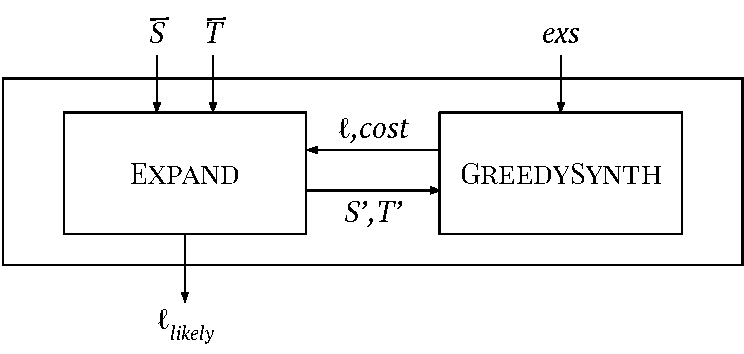
\includegraphics[width=.5\textwidth]{high-level-algorithm.pdf}
%  \caption{Schematic Diagram for \SOptician. Regular expressions \Regex and
%    \RegexAlt, and a set of examples \Examples, are provided as input. \RXSearch
%    searches through stochastic regular expression pairs, equivalent to the
%    originals, and proposes them to \GreedySynth. \GreedySynth finds a lens,
%    typed between the generated equivalent pairs. When \RXSearch determines it
%    has an optimal lens, it returns that lens.}
%  \label{fig:high-level-algorithm}
%\end{figure}
%
%\bcp{It gets rather technical and incomprehensible for the next three
%  paragraphs...} 
%
%We develop an algorithm that synthesizes a low-cost lens, shown in
%Figure~\ref{fig:high-level-algorithm}. This algorithm consists of two
%communicating synthesizers, one that proposes candidate stochastic regular
%expression pairs that it thinks will align well, and one that greedily searches
%for a lens between those two regular expressions that minimizes cost and does
%not traverse star-related equivalences\bcp{???}. When the first algorithm is content with
%the lens it has found, it returns that lens. 
%
%\bcp{Make clear that these algorithms are based on earlier / published ones.}Our first algorithm, \RXSearch, proposes candidate stochastic regular
%expressions. These candidate stochastic regular expressions are generated by
%traversing \emph{star semiring} equivalences on stochastic regular expressions.
%These proposed stochastic regular expression pairs have equivalent languages and
%probability distributions as the original ones: we prove that the star-semiring
%rewrites this synthesizer applies are sound rewrites on stochastic regular
%expressions.
%
%Our second algorithm, \GreedySynth, utilizes alternative languages for
%stochastic regular expressions and lenses, \emph{stochastic DNF regular
%  expressions} and \emph{symmetric DNF lenses}. While these languages are hard
%to read and understand, they are highly normalized and permit an efficient
%type-directed synthesis algorithm. We develop our cost metric on DNF lenses, and
%provide a greedy algorithm that tries to find a symmetric DNF lens of minimal
%cost. The synthesized symmetric DNF lens is then converted to a lens in the
%original simple symmetric lens language.
%
%
%We evaluate our algorithm on a benchmark suite consisting of synchronizing file
%formats from configuration files, application-specific data storage files, and
%data cleaning tasks. We find that our algorithm is able to synthesize each of
%these lenses in under 20 seconds.
%
%In summary, our contributions are:
%\begin{enumerate}
%\item We develop \emph{simple symmetric lenses} a new formulation for
%  bidirectional programs that can project data from both sides~(\S\ref{sec:overview}),
%  and describe a language that expresses such lenses on string
%  data~(\S\ref{sec:ssl}).  \bcp{A new language, or a variant of
%    Hofmann/Pierce/Wagner?} 
%\item We develop a means to traverse stochastic regular expression equivalences,
%  while preserving probability distributions and
%  languages~(\S\ref{subsec:stoch-rx}).
%\item We develop stochastic DNF regular expressions and DNF
%  lenses~(\S\ref{subsec:greedy-synth}). We develop a sound algorithm for
%  converting stochastic regular expressions to stochastic DNF regular
%  expressions and a information-theoretic cost metric on DNF lenses.
%\item We extended Boomerang with our simple symmetric lens combinators, and
%  integrated our algorithm with the Optician synthesis system within Boomerang,
%  allowing synthesis tasks as Boomerang
%  expressions~(\S\ref{sec:implementation}).
%\item We evaluate our algorithm on a benchmark suite consisting of synchronizing
%  file formats from configuration files, application-specific data storage
%  files, and data cleaning tasks (\S\ref{sec:evaluation}).  \bcp{... and
%    conclude what?}
%\end{enumerate}

%%% Local Variables:
%%% TeX-master: "main"
%%% End:
